\UseRawInputEncoding
\documentclass[12pt, a4paper, oneside]{book}

\usepackage{helvet}
\usepackage{hyperref}
\usepackage{graphics}
\usepackage{graphicx}
\usepackage{listings}
\usepackage{textcomp}
\usepackage[
	a4paper,
	outer=2.5cm,
	inner=2.5cm,
	top=2.5cm,
	bottom=2.5cm
]{geometry}
\usepackage{float}
\usepackage{tabularx}
\usepackage{xcolor}
\usepackage{amsmath}
\usepackage{framed}
\usepackage{subcaption}
\usepackage{shorttoc}
\usepackage{url}
\usepackage{dirtytalk}

\definecolor{grey}{rgb}{0.9, 0.9, 0.9}
\definecolor{dkgreen}{rgb}{0,0.6,0}
\definecolor{dkred}{rgb}{0.6,0,0.0}

\lstdefinestyle{DOS}
{
    backgroundcolor=\color{black},
    basicstyle=\scriptsize\color{white}\ttfamily,
    stringstyle=\color{white},
    keywords={}
}

\lstdefinestyle{makefile}
{
    numberblanklines=false,
    language=make,
    tabsize=4,
    keywordstyle=\color{red},
    identifierstyle= %plain identifiers for make
}

\lstset{
  language=Python,                % the language of the code
  escapeinside={\%*}{*)},
  basicstyle=\footnotesize\ttfamily,
  numbers=left,                   % where to put the line-numbers
  stepnumber=1,                   % the step between two line-numbers. If it's 1, each line
  numbersep=5pt,                  % how far the line-numbers are from the code
  backgroundcolor=\color{white},      % choose the background color. You must add \usepackage{color}
  showspaces=false,               % show spaces adding particular underscores
  showstringspaces=false,         % underline spaces within strings
  showtabs=false,                 % show tabs within strings adding particular underscores
  frame=single,                   % adds a frame around the code
  rulecolor=\color{black},        % if not set, the frame-color may be changed on line-breaks within not-black text (e.g. comments (green here))
  tabsize=2,                      % sets default tabsize to 2 spaces
  captionpos=b,                   % sets the caption-position to bottom
  breaklines=true,                % sets automatic line breaking
  breakatwhitespace=false,        % sets if automatic breaks should only happen at whitespace
  keywordstyle=\color{blue},          % keyword style
  commentstyle=\color{dkgreen},       % comment style
  stringstyle=\color{dkred},         % string literal style
  columns=fixed,
  extendedchars=true,
  frame=single,
}

\begin{document}
\clearpage
\newcommand\nbvspace[1][3]{\vspace*{\stretch{#1}}}
\newcommand\nbstretchyspace{\spaceskip0.5em plus 0.25em minus 0.25em}
\newcommand{\nbtitlestretch}{\spaceskip0.6em}
\pagestyle{empty}
\begin{center}
\bfseries
\nbvspace[1]
\Huge
{\nbtitlestretch\huge
Web Technologies: Client-Side}

\nbvspace[1]
\normalsize

COVERING DIVERSE TOPICS RELATED TO \\
CLIENT SIDE WEB DEVELOPMENT AND\\
FOCUSING ON THE CORE TRIUMVIRATE\\
OF HTML, CSS, \& JS

\nbvspace[1]
\small BY\\
\Large DR SIMON WELLS\\[0.5em]
%\footnotesize AUTHOR OF ``A WORKING ALGEBRA,'' ``WIRELESS TELEGRAPHY,\\
%ITS HISTORY, THEORY AND PRACTICE,'' ETC., ETC.

\nbvspace[2]

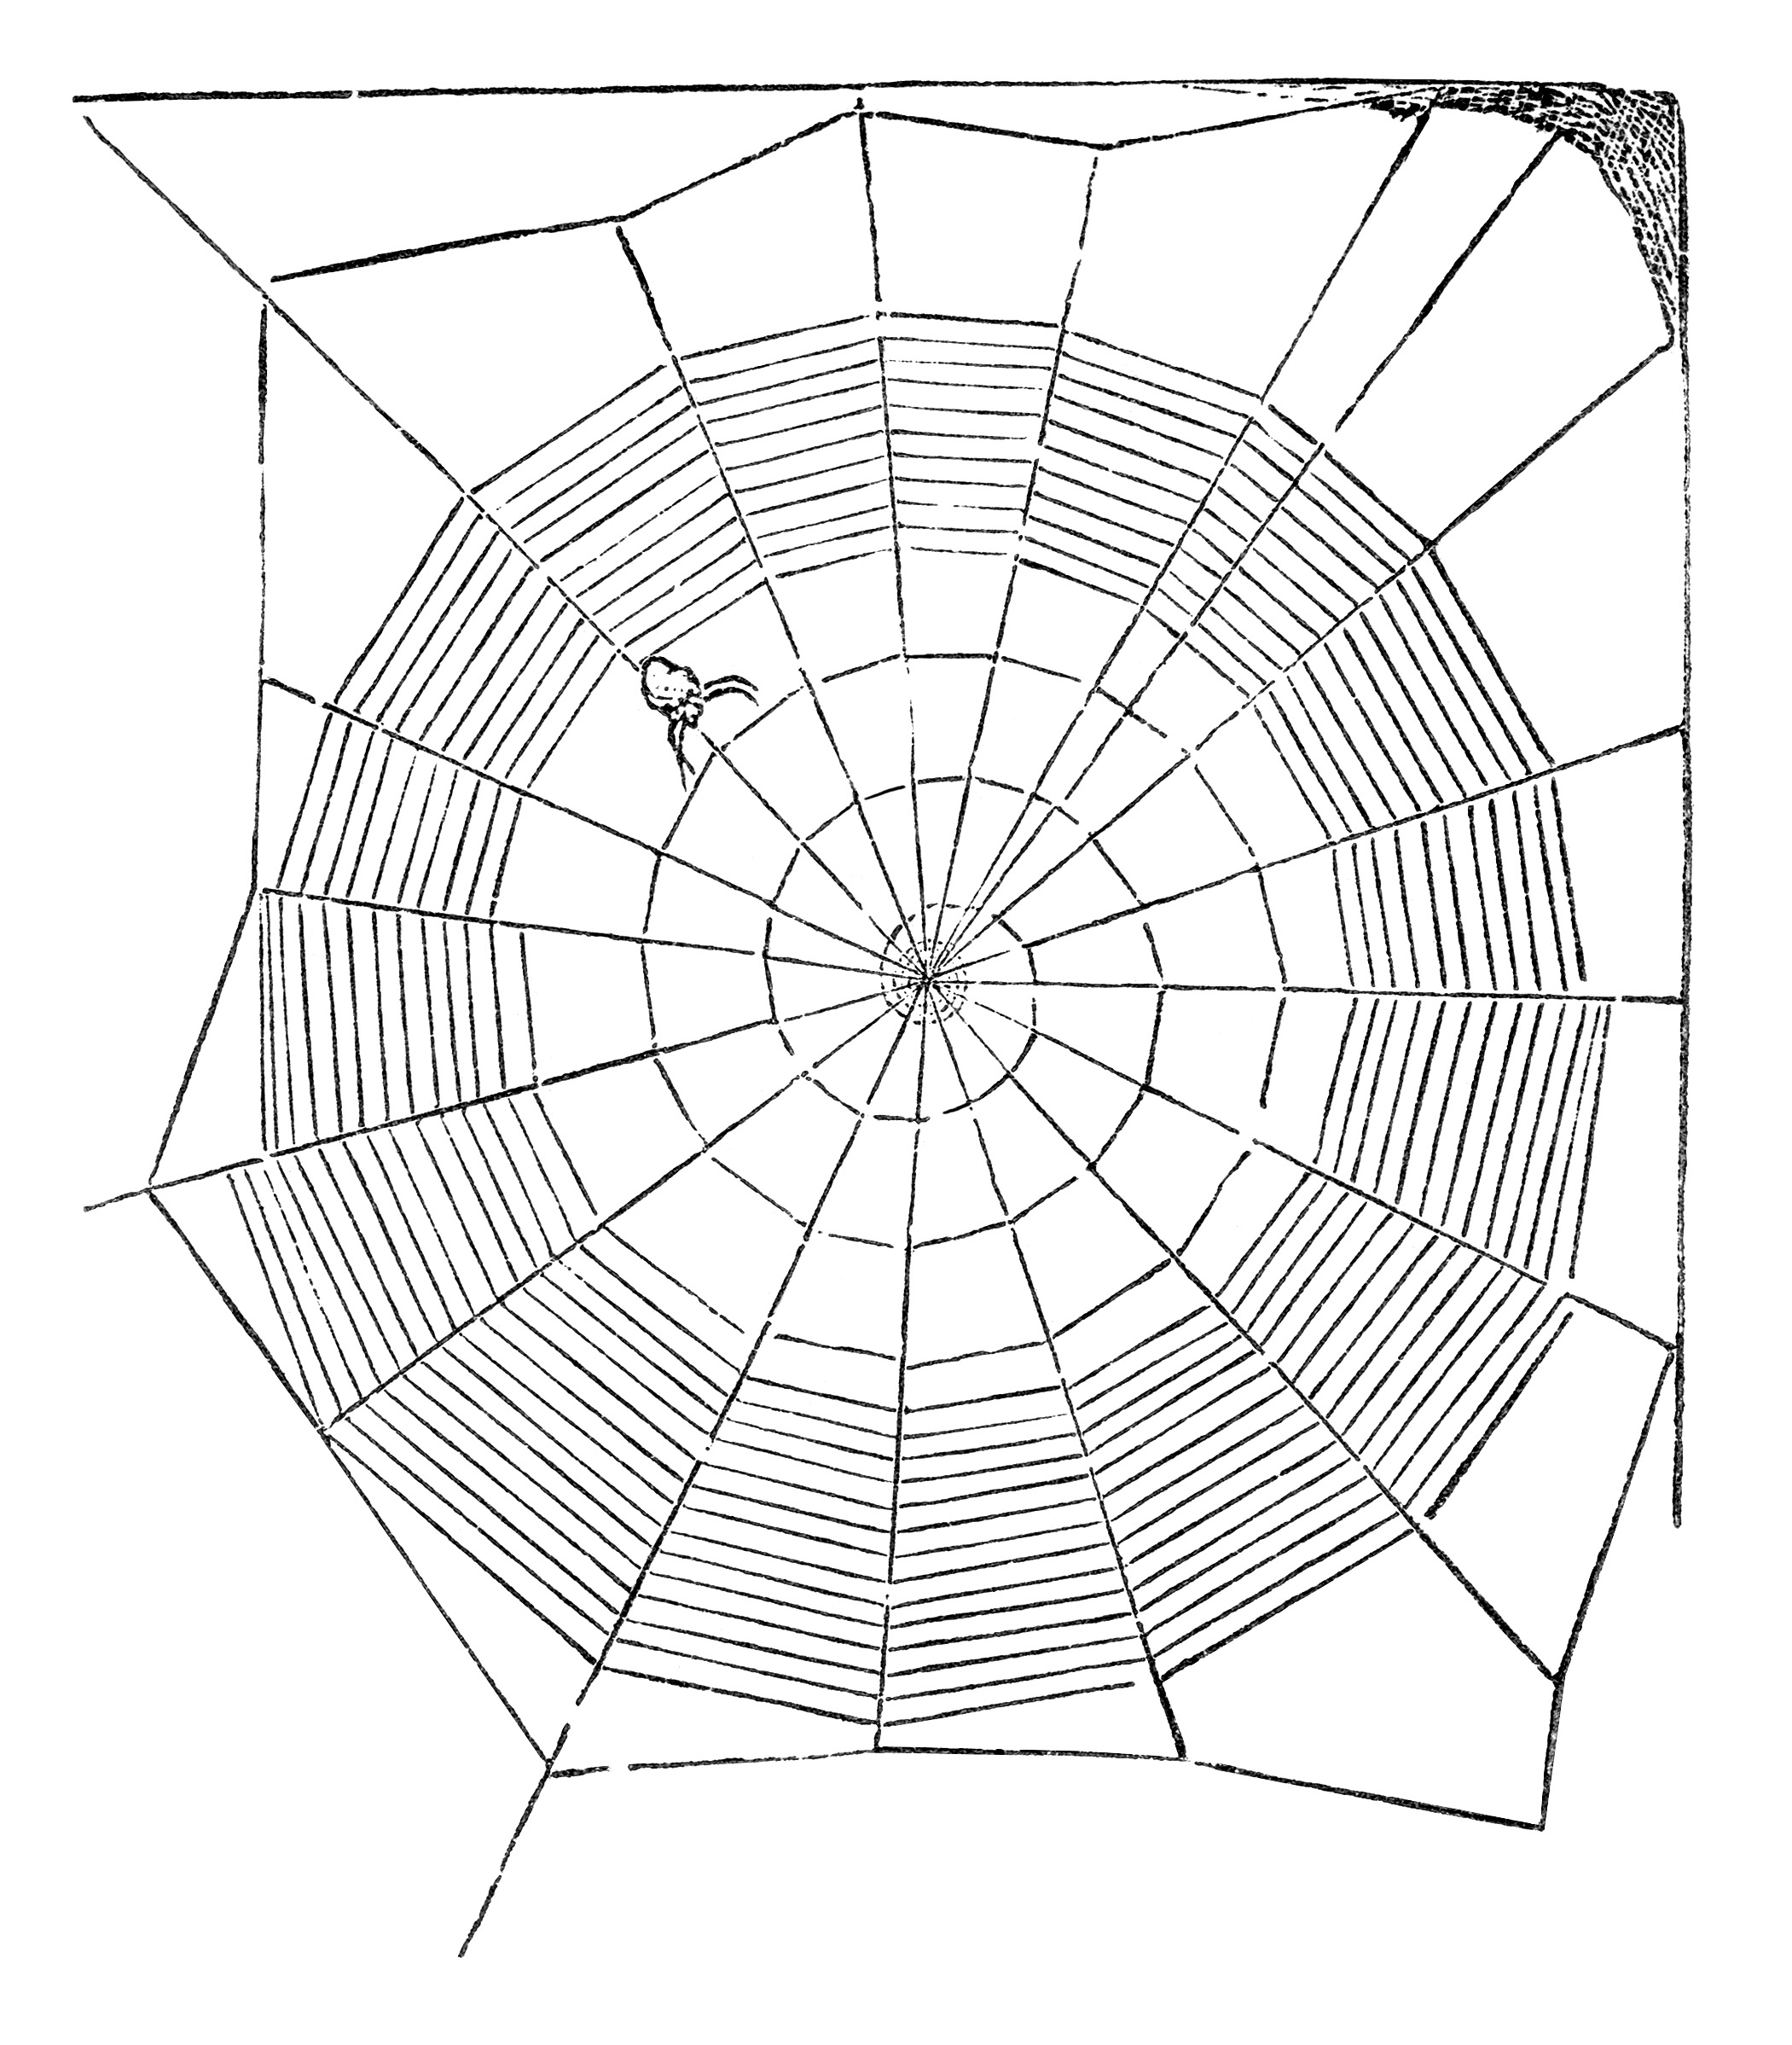
\includegraphics[width=2.5in]{figures/cover}
\nbvspace[3]
\normalsize

%SCOTLAND\\
\large
SESQUIPEDALIA VERBA PUBLISHING LTD
\nbvspace[1]
\end{center}


\setcounter{tocdepth}{2}
\cleardoublepage
\tableofcontents
\addtocontents{toc}{~\hfill\textbf{Page}\par}

\mainmatter

\chapter{Administrivia}

\section{Introduction}
\label{intro}

\paragraph{} Welcome to the Web Technologies module from Edinburgh Napier University. This module has a slightly different structure to many modules so it's worth reading through this guidance before you get stuck into the good stuff.

%\paragraph{} This module is about the Web, what the Web is, what we can currently do with the Web, and what the Web might be like in the future. Rather than focus on the user side of web technology, such as CSS and Javascript, which we've all probably seen in other modules (particularly \emph{web tech}, the pre-requisite for this module), we are going to take a more holistic approach and examine both the server and the client side. We shall look at HTTP (the core of all web technologies) and learn how APIs, Web Services, \& RESTful architectures are built to move data around. We will then delve into some more topical discussions, starting with security \& privacy on the web, then looking at adding intelligence (Semantic Web), adding increased, scalable interaction (Realtime Web) and private, anonymous, and un-censorable web-technologies (Dark Web). We wrap up the module by examining a few technologies that might form the basis of future web capabilities like Blockchain and IPFS. Throughout the module you should be using the topics as a starting point. A starting point for your own, self-directed, exploration of the topic in more depth. Because we can only really survey any given aspect during contact time; the real knowledge comes from you digging into it in depth. Also a starting point for you to critically reflect on your own experiences and responses to the topics and issues that we raise in class. Whilst the Web itself is a technical mechanism, a tool for moving data around, it also operates in a very complex socio-technical context that currently affects, and will likely affect to an even larger degree in the future, all our lives.

%\paragraph{} Lectures and labs will not necessarily align neatly, the labs will progress, on a week-by-week and chapter-by-chapter basis to form a first course in ``\emph{developing server side web-apps using Python and associated professional practises in a Linux-based environment}''. The lectures will summarise some of this material, providing an opportunity to talk over what we learned in the lab, but primarily, the lectures are an opportunity for us to discuss many other aspects of the Web, focussing in particular on two aspects. Firstly, the structure of the existing Web. Secondly the various facets of Web technologies that influence or alter the way that we use, manipulate, navigate, and share information. These break down into a series of named facets: the semantic web, the realtime web, the dark web, and the permanent web, each of which imposes its own constraints on and proffers opportunities for what the Web is and can do. By looking at each of these in turn we should gain some insight into how the Web is developing, the directions it might take in the future, and perhaps, suggest areas that we can usefully and positively affect.

\paragraph{} How should we use this workbook? Ideally we would work through it on a chapter-by-chapter basis supplementing our work with background reading and wider exploration of each topic introducted. Some chapters will take longer to complete than others, and other chapters will need to be returned to multiple times. This is particularly true for the first two chapters. To learn both Linux and Python in a fortnight is a tall order so I'd suggest working iteratively, do enough to make some progress, then frequently return to the respective chapters to learn a little more, usually by following the links and footnotes to further practise materials.

\paragraph{} In the first week work through the first chapter in the lab section of the workbook. You can read ahead if you want but don't try to run any Flask web-apps on the dev server until you've been assigned your personal virtual server to run your own web-apps on. This week is mostly concerned with the foundation of our learning environment. Logging in, learning to navigate and do simple tasks at the command line, using a non-gui text editor, and using Git. There are links, usually in footnotes, throughout the chapter, for example, to practise the Linux command line then there are online web sites like the \emph{LinuxZoo}\footnote{\url{http://www.linuxzoo.net}} that you can use to practise your skills. Similarly, the links to Vim practise tutorials, particularly the Vim game, will help you practise the skills you need to work efficiently in subsequent weeks. Finally, make sure to work through the linked Git tutorials and ensure that you are confident that you understand each of these tools and their place within the learning environment before moving on to subsequent chapters. 

\paragraph{} Each chapter is meant to cover about an entire week of study, so don't rush through things within the scheduled lab session just to tell yourself the you've done all the work. As I mentioned in the introduction, topics, whether in lectures or labs are meant to be a starting place, a framework to guide your self-directed study, but not the totality of your learning. 

\paragraph{} In subsequent weeks you will start to build knowledge of the Python language and the Flask library which provides functionality for building server-hosted web-apps. The next chapter, on Python, is meant to cover at least a weeks work and deliberate practise. Mostly that week is concerned with developing basic skills in a new language, Python, which is actually quite a challenge. This is not because Python is particularly difficult but because learning a computer language well takes time and effort and you have to start somewhere. Subsequent weeks will require you to work through various chapters of the workbook. You will find that as you progress you will want to skip ahead to different sections, especially once the assessments are released and you want to include specific functionality in your coursework. So after about chapter 3 I expect that many of you will navigate your own path through the remainder of the workbook. The only proviso is that you should aim to have worked through every chapter by the end of the module.


\section{Reading This Book}
\label{readme}
\paragraph{} 

\begin{figure}[H]
\centering
\includegraphics[width=0.8\textwidth]{figures/reading-order.pdf}
\label{fig:reading-order}
\end{figure}



\chapter{The World Wide Web}
\label{www}
\paragraph{} In this unit we begin the module with an introduction to the Web and an overview of the technologies which it comprises. From this starting point we can use subsequent units to take deeper dives into the various specific tools and technologies so that we can build a balanced and professional toolbox of Web related skills. You've probably used the web before, even if only to access this module, but more likely it is a part of your daily life so you probably have a number of preconceived ideas about how it works, how it should work, and where it is annoying and in need of improvement. You might also have had some previous experience in the Web. This is good but not necessary. We'll start from scratch in our approach to the Web which is an opportunity to reconfirm your ideas if you already know some parts and an opportunity to build new skills and understanding otherwise. 
%Practical activities for this unit are in the linked pdf file (unit1_activities.pdf). You should balance your time between working through the reading and reflective exercises in this unit on Moodle, and working through the linked activities separately in order to develop your practical skills.
 
\paragraph{} Before we can go anywhere, we should really know how we got here. This is important because the Web has been developed incrementally over around 30 years. However it is also based upon ideas that go back to at least 1945 when Vannevar Bush described the ideas of Hypertext and an associated machine, the Memex, and probably earlier. The Web, on the most basic level is really a conceptual tool for making knowledge capture, communication, and reasoning easier, but over the years there has been feature creep to do an awful lot more.
We are going to spend a little time in this unit doing a potted history of the Internet, the Web, Hypertext, DOM, \& Basic Web Architecture (Servers \& Clients). We'll then build upon, and iterate over this, iteratively deepening our knowledge and skills in subsequent units.
Whilst you are reading and thinking, consider the following question, What happened technologically \& socially, that lead to the situation we are in now and gave us the Web that we have now? 
By thinking about these things, and considering the tools that underpin the Web, we begin to construct a framework for understanding how it all fits together so that we can better use and develop our skills later.
 
vThis specific unit covers a lot of ground and it can be difficult to see how it all fits together at first. We will cover the following topics: Communication, The Internet, Internet Protocols, HTTP, Hypertext, the invention of the Web, HTML, Servers, Web-clients, Browsers, Basic Web Architecture, the client-server model, and the DOM. All are important topics when considering the Web, especially the process of getting a web page from a given Internet server to your web browser There is no single route through all of these topics as, like the web itself, they form a network of interconnected topics which each play their part in that story of getting a file from a remote server and turning it into a page in your browser. Let's consider a few scenarios:
For example, there is a historical story involving how people have thought about communicating ideas. Most ideas are hierarchically organised and related to other ideas, which lead to concepts for arranging ideas as "hypertext".

\paragraph{} There is also a computer communication story. For a computer to be able to move (communicate) information from one place to another it requires a network of multiple computers (the Internet) and agreements on how the communication should occur. These agreements are known as protocols. The Web relies on a hierarchy of protocols for things like finding another computer (using addresses call Internet Protocol, or IP, addresses), then transporting messages between the computers once they can find each other (using the Transmission Control Protocol ,or TCP), then because there are lots of different kinds of messages that computers can understand, they need a protocol for communicating web pages instead of other messages such as email data, or instant messages. This is achieved using the HyperText Transport Protocol (HTTP) which is responsible for moving Web data around. But Web data can comprise lots of different things, including the page itself (using HTML), the way the page should be presented (defined using CSS), and any dynamic functionality that the page should have (using JS).
There is also an organisational story. Whilst every computer on the Internet has an IP address (is a part of the Internet) not all of them are parts of the Web. Also, different machines play different roles, i.e. in requesting a page, serving a page, and displaying a page. So a server will provide pages to clients who make requests, and requests are made by software called "user agents" the most common type of which is the users browser. The browser and server are organised in terms of a client server organisational model.
As you go through the remaining parts of this unit, it can be worth returning to this overview to try to understand how the various parts relate to each other.


\paragraph{} So let's start by considering communication. The primary thing that the Web does is to communicate information from one place to another. For a computer to be able to communicate this information usefully, that is so that the computers at each end of the communication can understand what to do with the information, there needs to be an agreement on how the communication should proceed and how the  contents of the communication should be structured and understood. This shouldn't surprise you. Think about how you communicate with other people. For most of us, the primary means is through language. Amongst other things, successful communication between people using language involves a shared language, and some common vocabulary and understanding of the domain that the people are communicating about. The advantage that people have is that they have a brain which can solve problems and gloss over the gaps in understanding. Computers don't have this advantage, they need every aspect to be precisely specified in an unambiguous fashion.

\paragraph{} The solution, for computers is to use protocols to underpin communication. Protocols are agreements for how to communicate and they closely specify, for everything within the scope of a communication, exactly what is legal, and what is not. This means essentially that a protocol defines what a message, from one speaker to another can consist of. Any message that doesn't fit what the protocol defines is considered wrong and there are various ways to handle such wrong, garbled, incomplete, etc. messages. Computer protocols are agreements that are specified with sufficient clarity and lack of ambiguity that a computer can follow them automatically.

\paragraph{} The Internet and the Web are really just communication methods (protocols) - agreements for how two machines can exchange information. The Web itself is just one specific way that machines can exchange information. Let's now explore a couple of these concepts in some more detail...

\section{The Internet}

\paragraph{} The Internet is a global system of interconnected computer networks. Over the years there have been many different protocols underpinning computer networks, because what else is a network but a way to move information, or communicate information, between different machines. Over the years some of these protocols have become standard, and others have become obsolete. The modern Internet is currently built on a limited number of shared \& agreed protocols. These are the Internet Protocol suite which comprises the Transmission Control Protocol (TCP) and the Internet Protocol (IP). Together these are often referred to as "TCP/IP". 

\paragraph{} IP is used to govern how machines on the Internet find each other. To do this they use IP addresses, essentially numbers that are formatted as dotted-quad layouts like this:\\
	134.16.46.98
\paragraph{} Occasionally you might see IP addresses in your browsers address bar. Every Web site is stored on and "served" by web server software. This software runs on a hardware server which is not only a part of the web but is also a part of the Internet, i.e. every web site is a part of the Internet. Every web host is a part of the Internet. However, not every Internet host is a part of the web. The Internet is much bigger and incorporates functionality that is not part of the web. 
\paragraph{} Every Internet host has an IP address which is used to find other machines. The exact mechanism for finding machines from their IP address, which is literally about identifying a specific piece of hardware somewhere in the world, is outside the scope of this module, but the correct functioning of IP is essential to the working of the web. Think of an IP address as being analogous to, but not exactly the same as a postal address or a phone number, or a GPS location, a way to identify one entity, to distinguish it from others, and to locate it.
\paragraph{} TCP works with but is different to IP. Once you've located a machine, via its IP address, TCP is used to communicate data between that machine and any other machine that has an IP address. TCP is the basic mechanism for transmitting data between Internet hosts and controlling that process. Importantly, if something goes wrong during transmission, TCP has lots of mechanisms for repairing the communication. It is designed to be reliable so that a piece of software can send information, i.e. a message, to another host with guarantees that the communication will either fail or succeed. The sender and receiver don't have to worry about how the data actually gets from one to the other.
\paragraph{} An important concept here is that each protocol has its own responsibilities and they are designed to work both independently but complementary to each other. We can't send a message without knowing where it's going, but just knowing the destination doesn't necessarily tell us how to get the message to that destination. We should also consider that these protocols not only work independently but still in a complementary fashion, but also that they are designed to be layered. That is the current Web assumes that there are lower level protocols which are responsible for finding other Internet hosts, moving data to them, and returning the results. TCP/IP don't need to be the lower level protocols, and others exist, but they are the default that the modern Internet and Web currently use.
\paragraph{} The development of TCIP/IP and other networking protocols specific to the Internet dates back to research in the 1960’s which was commissioned by the US government. The aim was to build robust, fault tolerant communication via computer networks. To a large degree this has succeeded. The World Wide Web (or just Web) is just one information resource/service that communicates using the Internet (although people often use the terms interchangeably).


\section{Internet Protocols}
\paragraph{} In the last section we discussed how the Internet and the Web are built on the idea of layers of protocols. Formally there is a seven layer model called the OSI model that defines all of these layers and their various responsibilities. We don't need to know about all of them for this module so will concentrate on just those necessary to understand how the Web fits into the idea of the Internet and networks.
\paragraph{} Let's explore this a little further. On the lowest level that we'll consider here is the link layer, think of this as both the physical infrastructure, such as your WiFi or ethernet cable. It is concerned mostly with reliably moving information from place to place. Although this seems similar to TCP above, it is much lower level and the main difference is that the link layer doesn't care about how that information is broken up into packets or reassembled, it only cares that the stream of data it is given is reproduced at the other end. In comparison, TCP takes a particular approach to breaking up the data to transmit into packets, and uses specific algorithms to reassemble those packets into a whole at the other end, and also to identify and retransmit lost or broken packets. A similar protocol that works at the same level as TCP is the User Datagram Protocol (UDP) which doesn't provide the same guarantees on message integrity that TCP does. However the trade-off here is that UDP can be more efficient and faster to communicate information, with all of the risks associated with a send and forget communication protocol. We have these different protocols to enable us to use computer networks to communicate different information in different ways. Perhaps consider it as analogous to the difference between the different ways of physically sending messages around the world. We could write a postcard, or a letter in an envelope, a package or box, right up to a shipping container (and possibly other mechanisms as well but these are fairly standard).
\paragraph{} As we talked about before, once we have two networked machines (link layer) that can transmit data, they need a mechanism that enables them to address messages to specific machines, which is the role of the Internet layer and IP. Once we have a machine that we can identify individually we can use the transport layer (TCP) to move data in a specific way to the destination. It is only at this point, once we have the link, internet, and transport layers that we look at the application layer. It is this layer at which the Web protocols operate. The HyperText Transport Protocol (HTTP) is one example of this that we will investigate next but there are lots of other applications layer protocols which govern other tasks like email (the IMAP and POP protocols) or turning domain names (web addresses) into IP addresses so that, given a web address or URL (different names for the same thing) we can tell the IP protocol which machine we want to communicate with. Although people generally think of websites in terms of domain names, our computers only care about IP addresses when it comes to finding a given web server.
\paragraph{} To summarise, we have:
\begin{itemize}
\item Link Layer: Ethernet/Wifi
\item Internet Layer: IP
\item Transport Layer: TCP
\item Application Layer: DNS, HTTP, IMAP, POP 
\end{itemize}


\section{The HyperText Transfer Protocol (HTTP)}
\paragraph{} Just a little more on protocols before we consider some other aspects of the Web. The HyperText Transfer Protocol (HTTP) is our application layer protocol that is critical to facilitating the Web. Other protocols like TCP and IP don't care that the data they are transmitting or the machines between which they are moving the data are Web machines or not. Those protocols can transmit lots of data for different reasons and many of those reasons are not related to the Web.  When information arrives at a machine and is routed to software that understands HTTP it is treated as Web data. HTTP is concerned primarily with moving hypertext between Internet hosts. We'll consider what we mean by hypertext in the next section but for the moment we can think of it as being text documents. Although the modern web can manage to handle much more than just text the default is still for HyperText Markup Language (HTML) documents. HTTP is concerned with moving these documents around, requesting particular documents and processing the responses, and delegating the actual movement of the document to lower level protocols along the way. Note that HTTP does much more than just merely governing requesting documents and responding with the correct document. It also has the mechanism for responding in different ways depending upon the request made, or how successful the request was. It is this additional functionality that enables rich, server generated behaviour and on the fly page creation, but these aspects of HTTP are outside the scope of this module, although you are encouraged to do some additional background reading if it interests you. A good place to start is with the W3C specification if you want the gory details: \\
	\url{https://www.w3.org/Protocols/}
\paragraph{} HTTP is an application layer protocol for distributed and collaborative hypermedia/hypertext systems. It is based upon a request-response protocol that uses the client-server model. We'll investigate the client-server model in a little while but the basic idea is that the Client (i.e. your Web browser) makes a request. This is probably due to the user making a choice such as clicking on a link or typing in a web address. This request gets passed down the layers of the networking stack, transmitted to the remote machine, and heads back up the networking stack until it reaches the server software that understands HTTP.  Mostly though we can ignore the full stack and just consider that there is an HTTP server (software running on an Internet connected computer) that listens for requests and responds according to what the protocol allows. Any other response is problematic and will cause some form of error or failure in the communication.

\paragraph{} The HTTP Server stores resources and returns a response that may include providing access to those resources. For our purposes in this module those resources should be considered to be the things that you'd commonly expect a web site to provide, e.g. HTML pages, associated files in the CSS and JS languages that the HTML pages reference, and any other media like images, videos, or audio that the pages want to make use of.
\paragraph{} These request-response cycles occur as part of an HTTP Session. This is a sequence of request-response transactions transmitted over TCP.  One thing to note at this point is that Internet hosts can listen on different ports. The default port for the Web is port 80. In fact it is so common that most browsers don't display that the address it is connecting to is listening on port 80. A web client can connects to any legal port on any legal IP address. HTTP servers listen on that port. Whilst the default is 80 you might occasionally see other ports in your address bar, for example 8080 which is also reasonably common but some development servers run on other ports like 5000. If you see other ports, don't worry.

\paragraph{} HTTP requests are more than just a simple request to retrieve a web page, They can also involve lots of other request Methods. These methods are usually referred to as  HTTP verbs, e.g. GET, HEAD, POST, PUT, DELETE, OPTIONS, and PATCH to name a few. These verbs are essentially actions that the request is asking to be performed. The most common is HTTP GET. This is asking to retrieve or "GET" the resource (web page or HTML document) that is being asked for and return it to the client. A client makes a request and the requested resources is transmitted back to the client. What is transmitted between the client and server though is just plain text. HTML web pages are plain text, CSS files are plain text, and javascript files are plain text. They are readable and understandable by people. If you were to eavesdrop on the connection between client and server you would see text passing by containing the HTML, CSS, or JS content of the files that are being requested and then "served" up. Note that modern versions of HTTP will retrieve binary files, e.g. for audio and video, but the default is for plain text, a simple and robust encoding mechanism that is easily inspectable without specialised tools. It is this focus on plain text file, the same kind of files that any text editor can produce, which is arguably a part of making the Web so successful. Anyone with a text editor can produce the files that will make up a web page. If they then put those pages on a web server, then voila, you have published a web site.
\paragraph{} Before we finish up this introduction to HTTP, note that by default HTTP is insecure. The transmission of information is in plain text and any one machine between source and destination could intercept or manipulate it. This risk has largely been mitigated by the use of secure variants of HTTP, such as HyperText Transfer Protocol Secure (HTTPS) \& HTTP Strict Transport Security (HSTS). Browsers are slowly moving towards defaulting to HTTPS addresses. The main difference between HTTPS and HSTS is that HSTS is more strict about how it deals with mixture of secure and insecure resources on a single page. HSTS mandates for a given page that all resources on that page are served securely. This is an example of the slow improvement of Web and Internet protocols.


\section{Hypertext}
\paragraph{} In the last section we discussed HTTP, a protocol for transferring hypertext resources between Internet hosts, but we didn't really define what we meant by hypertext. So let's square that away right now. Hypertext is a term that was coined byTed Nelson as part of the Xanadu research project sometime around 1965. This was as part of a model for linked content, the idea that a concept is related to other concepts and that it would be useful to create links between concepts within and between documents so that instead of reading a page, and then reading another page in linear fashion, as we traditionally read books, instead it is useful instead to be able to follow the thread of related ideas wherever they may take us. The following diagram illustrates this idea schematically, starting with the home page highlighted in orange, individual sections of text are linked to other pages which, in turn contains links to other pages, and so on.

\begin{figure}[H]
\centering
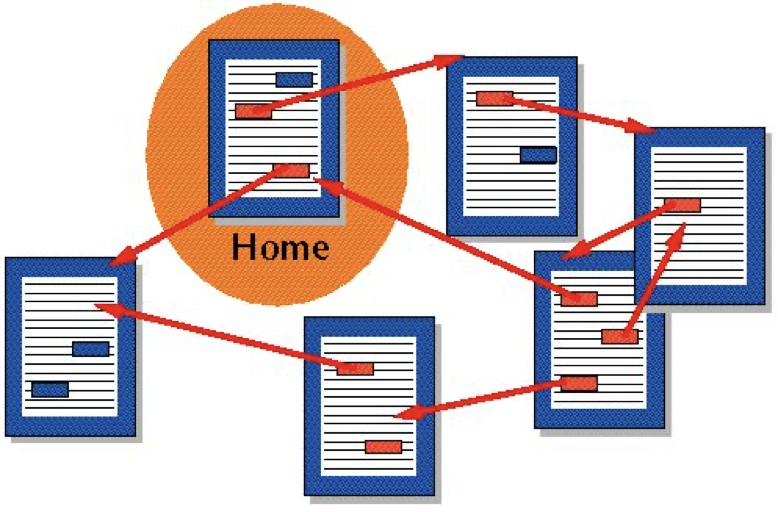
\includegraphics[width=0.4\textwidth]{figures/hypertext.png}
\label{fig:hypertext}
\end{figure}


\paragraph{} Ted Nelson didn't invent this idea though, an earlier incarnation which was visionary but came before the technology was capable was in an article by Vannevar Bush in 1945. Bush proposed the Memex, an attempt to turn this idea for turning information into a searchable and interlinked database of knowledge, however he was limited by the capabilities of 1940's technology. It is well worth reading Bush's article which can be found here:
	\url{https://www.theatlantic.com/magazine/archive/1945/07/as-we-may-think/303881/}

\paragraph{} But it is arguable that Bush didn't really invent this concept either. Before the Memex proposal we already had books that work in a similar, albeit manual and non-computational way. Dictionaries, Thesauri, and Encyclopedias also work in a similar way, referencing other sections and entries within themselves, other volumes in the collection, and other books. Encyclopedias in particular are interesting to consider because they often have summary books and indexes that give different ways to approach the articles contained within the encyclopedia proper.
\paragraph{} A modern incarnation of hypertext that is quite well defined and circumscribed is Wikipedia. Consider how you start on one Wikipedia page and then follow links to other pages until you've lost an entire afternoon discovering things you never thought that you'd want to know. This is hypertext. Text is displayed on an electronic device that incorporates references, called Hyperlinks, to other text. These Hyperlinks can be followed or navigated immediately. By doing this, text becomes non-linear as a result - instead of one page following the next we can jump between them, consuming them in whichever order makes most sense. 
\paragraph{} Note that the modern web goes beyond just links between text and other forms of media are often consumed on the Web now so you will often find the related term hypermedia used. The terms hypertext and hypermedia are frequently used interchangeably.
\paragraph{} One implementation of the hypertext idea is in HTML.  Whilst the bulk of HTML is about describing or "marking up" text documents one part of HTML concerns defining links within and between documents. Even just getting this far into the module, you'll already have navigated a whole bunch of hyperlinks as you've "browsed the web". Browsing the web is just another phrase for following hyperlinks or using hypermedia. 
\paragraph{} So the Web itself is an implementation of a hypertext system as well. That said it isn't the only possible implementation of a hypertext system, it's just the most prevalent one that we have now. Perhaps we should now consider how we ended up with the particular implementation of a hypertext system that we call "the Web"?


\section{Invention of the Web}
\paragraph{} The Web, or more formally, the World Wide Web (WWW) is an implementation of a hypermedia system. It was invented in 1989 by Sir Tim Berners-Lee whilst he was working at CERN. This involved developing HTTP to move documents around and HTML to structure and define documents themselves, with embedded links between them. The first web browser was written in 1990 but it was 1992 before there was really a usable and publicly accessible web browser (but which was very different to what we have now).

\begin{figure}[H]
\centering
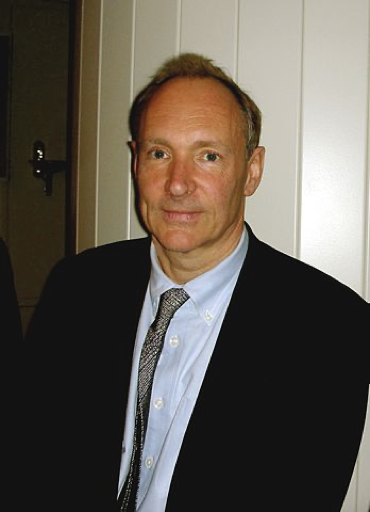
\includegraphics[width=0.8\textwidth]{figures/tim-berners-lee.png}
\label{fig:tim-berners-lee}
\end{figure}


\paragraph{} Berner-Lee's original aim was to build a system for sharing scientific research, e.g. amongst physicists. He was, after all, a scientist and the two core function of scientists are to find out things, and then, usually, to share those discoveries. Obviously we’ve come a long way since then and the Web has moved far beyond its original scientific information sharing ideals.
\paragraph{} The early Web was initially formatted text only, but rapidly moved to support images, audio, video, and other media types. This was driven by user need. Rather than a top down, well organised, grand plan for the Web, instead open protocols were created and shared. These are open because anyone can implement their own version of, for example, a web server, or a web browser, and because of the availability of the specifications for the protocols, these implementations are, generally, inter-operable. This means that my implementation of a web browser can understand the pages returned by your implementation of a web server.
\paragraph{} More information about the early days of the Web, and some resources such as the very first published web page can be found here:\\
	\url{https://home.cern/science/computing/birth-web}
\paragraph{} Given that we've spent a fair amount of time considering what the Web is, where it came from, and how it built on lower levels of networking infrastructure, perhaps we should now change tack a little bit. We've concentrated so far on how "web pages" are moved around, and the networking protocols needed to do this, but what actually is a  web page? That's our next topic....


\section{HTML}
\paragraph{} A web page is simply a document that can be retrieved from a web server. However, our browsers do more than merely retrieve documents and show them to us as plain text. We are used to web pages generally being perhaps quite colourful and often well presented (although the converse is also true). It seems that there is more to the Web than merely retrieving documents from the web server. It seems that the document itself is actually structured in a particular way and that the browser turns this structure into a particular presentation (perhaps with the aid of CSS and JavaScript as we'll see in subsequent units). It turns out that web pages are written using a particular language called the HyperText Markup Language (HTML). HTML is simply a language for turning text into structured hypertext using markup. Structured because it incorporates semantic information such as that a given sentence be treated as headings or paragraphs, or lists, and hypertext because it enables links to be defined between sections of text and other locations such as places within the current document or within other documents. HTML is called a language because it is a means for communication. There are many kinds of language, e.g. natural (e.g. English or Spanish) \& artificial (e.g. programming languages like Python or Javascript). There are also formal languages like HTML which are not general purpose programming languages because they lack the facility to handle things like variables or expressions but are better described as domain specific languages, languages that are devised to do something well in a given domain.
\paragraph{} We'll look at HTML in more detail in the next unit but for now we need to know that HTML handles  the domain of text. That is strings, or sequences of characters, that are encoded using an agreed format. Generally that format is UTF8. That is where the T in HTML comes from. So far I've glossed over what we mean by markup so let's put that straight right now. There are many ways to do markup and these are not specific to HTML and use a variety of techniques. The approach taken by HTML is to use Tags. HTML tags, or just "tags" are generally placed around the element being tagged, e.g. 
\begin{lstlisting}
    <h1>Hello</h1> 
\end{lstlisting}

\paragraph{} This places the $<$h1$>$ tag around the word "hello". Tags usually work in pairs to encapsulate a section of text so we indicate the closing tag with the '/' character. This just helps to pair them up so we can see where the encapsulated elements starts and ends. The angle brackets '$<$' and '$>$' indicate that they enclose a tag. In this case the specific tag is the h1 tag which is the name for heading level 1, which is basically the largest level of pre-defined heading. We will see this and more in the HTML unit but it is enough for now to realise that there are a lot of tags that pre-define, or capture,  different aspects of the text. Think of all of the documents you have ever read or written. Many will have similar elements like a title, various headings and sub-headings, paragraphs, and other typographical aspects. HTML tries to capture these so that the browser can process an incoming document and treat differently tagged parts of the HTML document in different way, perhaps by visualising and depicting the elements in various ways or by making different functionalities available, e.g. a hyperlink can be clicked upon to automate the process of navigating to the destination that the hyperlink points to.
\paragraph{} If you want to read ahead before you get to the HTML unit then it is well worth checking out the Mozilla HTML elements reference to see just what is available:
	\url{https://developer.mozilla.org/en-US/docs/Web/HTML/Element}

\paragraph{} Let's just consider the journey we've taken so far. We've considered the various protocols involved in putting a document on a server on the Internet so that it can be requested and treated as a Web page using HTTP. This involves lots of lower level protocols that are concerned with moving information reliably around the Internet. It's not just about moving the document around though, it's also about being able to understand the structure of that document and present it in an appropriate way using HTML. The final thread here is that hyperlinks within an HTML document present a shortcut to initialising the request and retrieval of further documents, via HTTP, so there is a functional and symbiotic link between HTTP and HTML. The next few topics are now going to round things out by considering how clients and servers are related to each other and, more importantly, what we mean by a "web server" or "web client".

\section{A Basic Web Architecture - The Client-Server Model}

\paragraph{} All of the topics that we've considered so far have lead us to this point. We now have all of the pieces  that we need to consider what we mean by a "client-server architecture of the web". Understanding this is important to knowing what is happening when you develop a web page or site and have multiple resources. A good developer will understand where their resources are located, how they are transmitted to the client, and when that occurs. This will help us to build a useful conceptual model of where our code is, whether HTML, CSS, or JS, when it is at rest and when it is executed, and the difference between each.
\paragraph{} In one sense the web architecture is very simple, there are web servers which listen for requests. They don't initiate communication but merely respond to incoming requests. Requests are made from clients. These can be browsers, or any other software, that speaks HTTP and can correctly formulate an HTTP request. Similarly a web, or HTTP, server is a server that speaks HTTP and can correctly respond to incoming HTTP requests. Clients make requests and servers respond.

\begin{figure}[H]
\centering
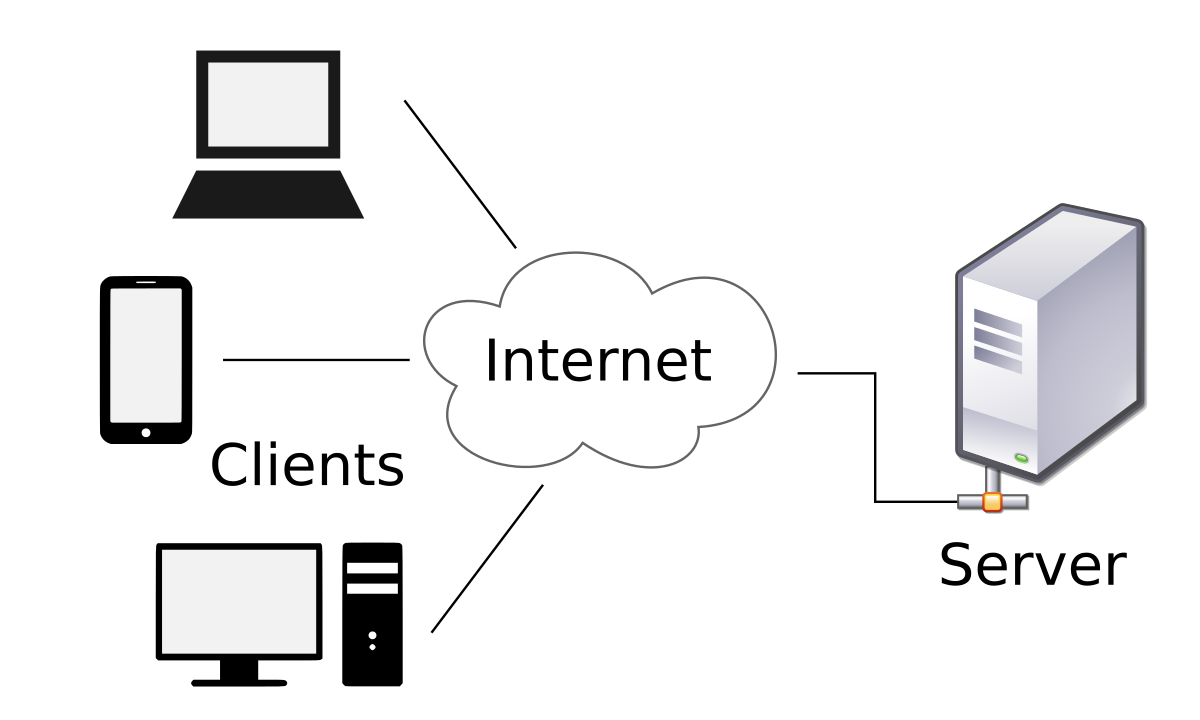
\includegraphics[width=0.8\textwidth]{figures/client-server-architecture.png}
\label{fig:client-server-architecture}
\end{figure}


\paragraph{} Web clients are merely software that communicate to a Web server by making requests. The communication is governed by HTTP. Web clients are often also referred to as user agents. A web browser is a particular type of user agent which acts on behalf of its user, i.e. acts as an agent, to satisfy their requests. There are other user agents, for example, command line tools that retrieve web page or other web resources using HTTP, but that don't render the results to the screen. For example, a web scraper or web indexer, is a user agent which collects web resources but does something else with them like, perhaps, building a database with the results. The reason we talk about web "clients" as well as user agents is because of the link to the client server architecture.
\paragraph{} To summarise, servers are software that responds to communications (HTTP requests) from clients (browsers).The response generally contains a document (HTML) that is transmitted back to the client as part of the response. Note that it can get (much) more complicated than that but this is a good starting place.


\section{Servers}
\paragraph{} The term server is heavily overloaded in computing. It can refer to hardware and it can also refer to software. Generally though we consider a server, whether hardware or software, to be acting in a particular role. That role is "serving", providing, or distributing data. Server software may run on server hardware, or might run incidentally on other hardware, for example, your laptop during development. Generally though we'll ignore the idea of server hardware in this module and just assume that on some level, all of our software is running somewhere appropriate. Server software isn't limited just to Web contexts though. For example, many database management systems work by using server software which responds to client requests. However a database, rather than speaking HTTP and HTML might instead use a query language like SQL or SPARQL. That said, some database servers also speak HTTP, an example of this is CouchDB which provides an API which can be accessed via a web browser. Whilst it's a little outside the scope of this module, it is worth considering just how many pieces of hardware out there could incorporate an HTTP server to provide a user interface to any browser rather than needing a specialised application. This is quite a democratising way to consider things and is especially exciting when we consider the idea of Internet of Things (IoT) and the notion that not only can the world provide data about what is happening to us, but things in the world can give us Web-based ways to interact with them.
\paragraph{} A server is, on the simplest interpretation, merely a piece of software that runs on a computer. It listens for messages and determines the right response to make (where the determination of request and response pairing is defined by the protocol).; we’ll l assume a server running on an Internet connected machine (so using TCP/ IP as lower level protocols). A web server is thus a server that listens for messages that are sent using web protocols (HTTP). By extension an email server is a server that listens for messages sent using email protocols (such as SMTP, IMAP, or POP).
\paragraph{} We've established that servers are responsive, they respond to something speaking to them by sending a message. If a server is listening then what is doing the speaking? 

\section{Web Clients \& User Agents}
\paragraph{} In the context of the Web, the software doing the speaking is the web client (or user agent). This is just another piece of software (nothing particularly special). Again, a web client just happens to speak HTTP but can initiate requests rather than merely waiting for them to arrive from other web clients. Other than this, a web client doesn't have to do anything more. It is useful to do something with the result of a request though. The result, the response, could just be logged, for example, the server responds with 200 OK. This would be enough if we were creating a web client that merely checked whether an HTTP server was alive and running correctly. A web spider (or search indexing agent) might retrieve pages from a site, then programmatically follow all the links to retrieve the pages that it links to and so on until it runs out of links to follow. Note that this is only a naive description of how a web spider might work. The spider would then do something else with the retrieved pages, perhaps building a database or analysing the page content for particular features. By contrast a web browser usually retrieves a single page then interprets the HTML content of the page to construct an internal, programmatic, representation of the page. This internal representation is the Document Object Model (DOM) which we will see soon. This DOM representation is then turned into, usually, graphical representation of the document. However, there are also text based browsers which manipulate the retrieved HTML document in a different way because they aren't visually based but are text oriented. Similarly a browser for the visually impaired might present an audio version of the page. The message to take away is that there is a lot more to the functionality of a web browser than merely retrieving pages and showing them to the user like a form of Internet PDF reader. Mobile apps are an increasingly popular web client. Frequently they will be retrieving data from a remote HTTP server (often as JSON documents rather than HTML documents) and then turning that data into a native application specific to the data retrieved rather than using a generic web browser. Essentially though, it is very easy for almost any piece of software to become a web client, it just needs to access, consume, or display web content, e.g. have the capability to talk usefully to an HTTP server.
\paragraph{} Let's now consider a specific type of web client, the web browser, possibly the most visible item of "web software" in our next topic.


\section{Web Browsers}
\paragraph{} Web browsers are software that not only speak HTTP so that they can retrieve HTML and other related documents from a web server but usually also contain some form of a layout engine that renders the web pages (HTML) into an appropriate form. This appropriate form is usually but not limited to the graphical web pages that we are used to from everyday web usage.
\paragraph{} The web browser is yet another invention from Berners-Lee. Having defined HTTP and HTML there was obviously a next step to create a user agent that could retrieve HTML from HTTP and then display it appropriately.
\paragraph{} Browsers are generally used to interactively navigate the public web but are also frequently used to access private networks, IoT interfaces, local file systems, and much more. 
\paragraph{} Browsers have also become a default cross-platform environment. Many items of software that might previously have been written as standalone desktop clients are now implemented as "web apps" that are generally accessible from any given web browser. This can solve many problems involved in the traditional development and distribution of software. For example, a new version of the software only has to be published to the web server and when the browser refreshes the page the new software is deployed. No more downloading, double clicking and installing or package managers required. However this is at the expense of different behaviours between various browsers which can affect user experience. There are also different performance characteristics when dealing with browsers compared with native applications. Also, browsers have been designed primarily for displaying web pages, which are essentially documents, with a particular flow of information and internal structure. This is not the same as a general graphical interface toolkit as might be used to develop for the desktop.
\paragraph{} There are many different producers of web browsers and the illustration gives you some idea of the prevalence and popularity of the more common of the various browsers. Note that this isn't entirely accurate because many browsers can identify as different user-agents, e.g. Firefox describing itself as Chrome, usually for compatibility. This is behaviour that is user-controlled and leads to the statistics on browser usage being a little uncertain.


\begin{figure}[H]
\centering
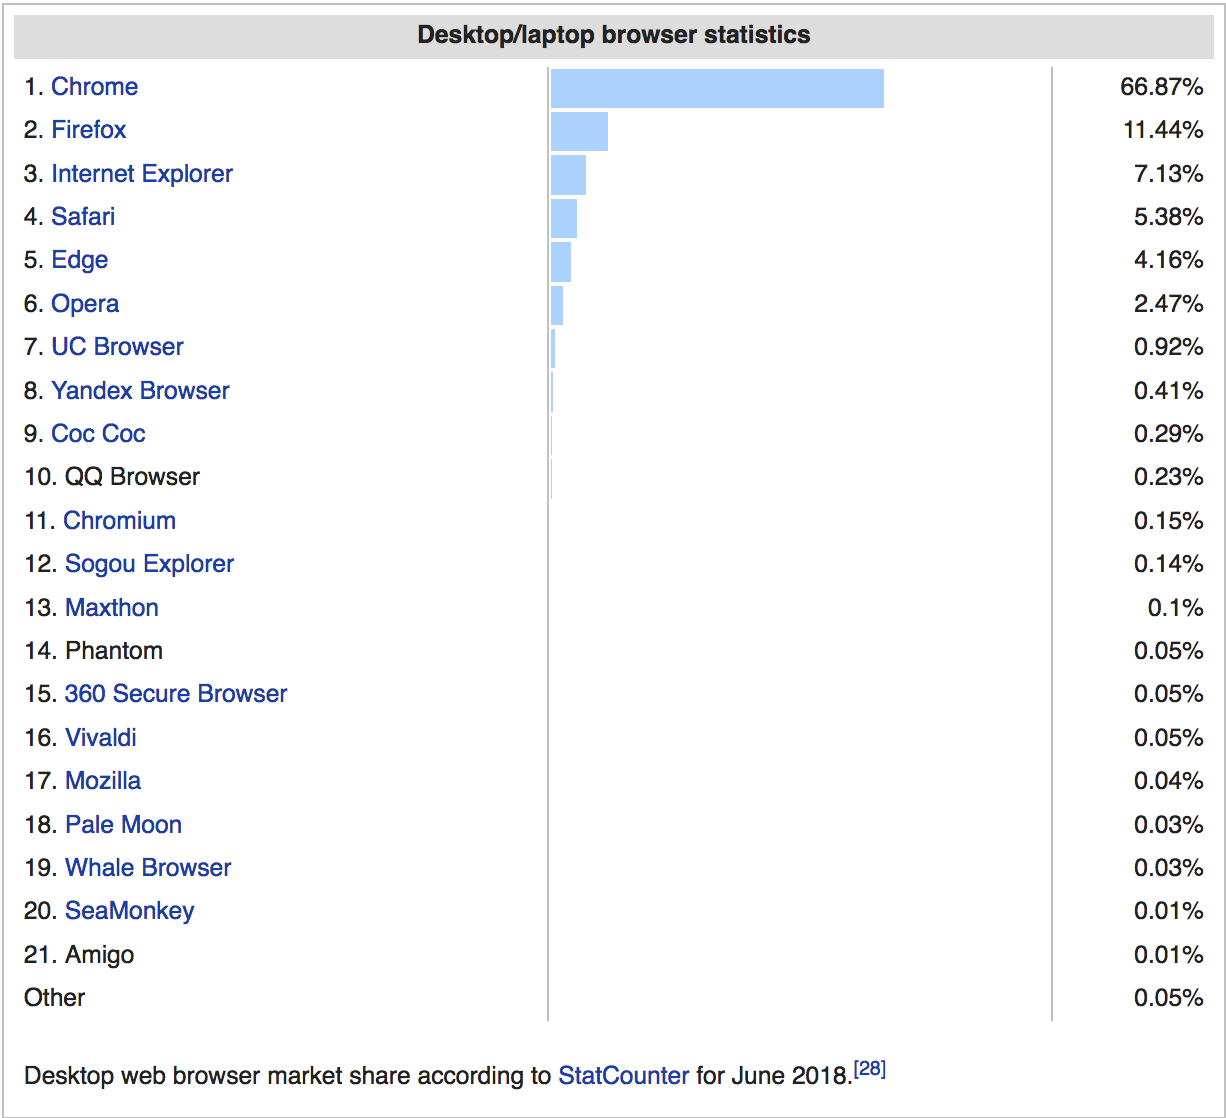
\includegraphics[width=0.8\textwidth]{figures/browser-stats.png}
\label{fig:browser-stats}
\end{figure}


\section{The Document Object Model (DOM)}
\paragraph{} We've made great progress now and have examined a lot of the technologies that are involved in retrieving a document from a web server and getting it into the browser. But what happens next?
\paragraph{} The HTML obviously needs to be altered from its default text based .html file into something that can be translated into the graphical display we are used to seeing in our web browsers. This is achieved by creating an intermediate model, named the Document Object Model (DOM).
\paragraph{} The DOM is a cross-platform, language independent Application Programming Interface (API). It parses the incoming HTML document, treating it as a tree data structure internally within your browser. The tree is formed due to the hierarchical and encapsulated nature of HTML tags where everything is enclosed within <html> tags at the top level. The <html> level encapsulates <head> and <body> tags which in turn encapsulates other tags, and so on, until everything is in place. This is heavily dependent upon the specific tags found in any given HTML document. HTML is parsed into this data structure to construct the DOM (for that document). Each part of this tree is represented internally to the browser as an object that can have various attributes and methods. These methods can then be called to manipulate the model, a process often referred to as manipulating the DOM. 
\paragraph{} The methods associated with the DOM provide an API that JavaScript can interact with to manipulate the current page. For example, Objects can be manipulated programmatically, e.g. using Javascript, and the results displayed in the view pane of the user agent (browser). The browser also provides other APIs for interacting with the environment from JavaScript but the DOM is a good place to start.
\paragraph{} It is also worth noting that the DOM and the HTML sources are not the same. You cannot rely on the HTML that you loaded initially being a good representation of what you see in the browser or what is represented internally in the DOM. When the HTML is parsed it is used to construct the DOM, but this model can then be manipulated by any linked JavaScript and also manipulated visually, or even hidden, through CSS. If you right click on a page in your web browser and select "view source" then you will see the original HTML that was retrieved from the web server. If instead of view source, you load the browser development tools then you can use these to inspect and manipulate the DOM, if you compare the two then you might notice that the DOM is not always identical to the source HTML.
\paragraph{} You can find a little more about using the Chrome dev tools to inspect the DOM here:
	\url{https://developers.google.com/web/tools/chrome-devtools/dom/}
\paragraph{} We will return to consideration of the DOM throughout the HTML, CSS, and JS topics in subsequent units. An awful lot of client-side javascript involves manipulating the DOM.

\section{Browser Developer Tools}
\paragraph{} Our final topic for this unit is to consider turning all of this theory into practice. We only really need a good editor and a good browser to get started with client-side Web development - Web IDE’s are often overkill for simple development.
\paragraph{} There are many browsers: Chrome, Chromium, Firefox, Safari, Opera, IE/Edge - but for this module we will focus on Chrome so that we all have a consistent development and learning environment. I'd still suggest having other browsers installed though so that you can compare behaviour between them.

\paragraph{} All newer browsers have support for some set of developer tools. Common Features of Developer Tools include the following:
\begin{itemize}
\item HTML \& DOM viewers \& editors
\item Web page assets, resources, network information 
\item Profiling \& Auditing
\item JavaScript Debugging \& Console 
\end{itemize}

\paragraph{} Chrome is currently very popular but it also pioneers many new ideas and directions for the future of the Web.
\paragraph{} It is fast, stable, and feature rich. It also has many tools to support developers - get access to the surface (the web page) but also the internals of the browser and the web page/application. We can launch the developer tools by following the procedure in this screenshot:

\begin{figure}[H]
\centering
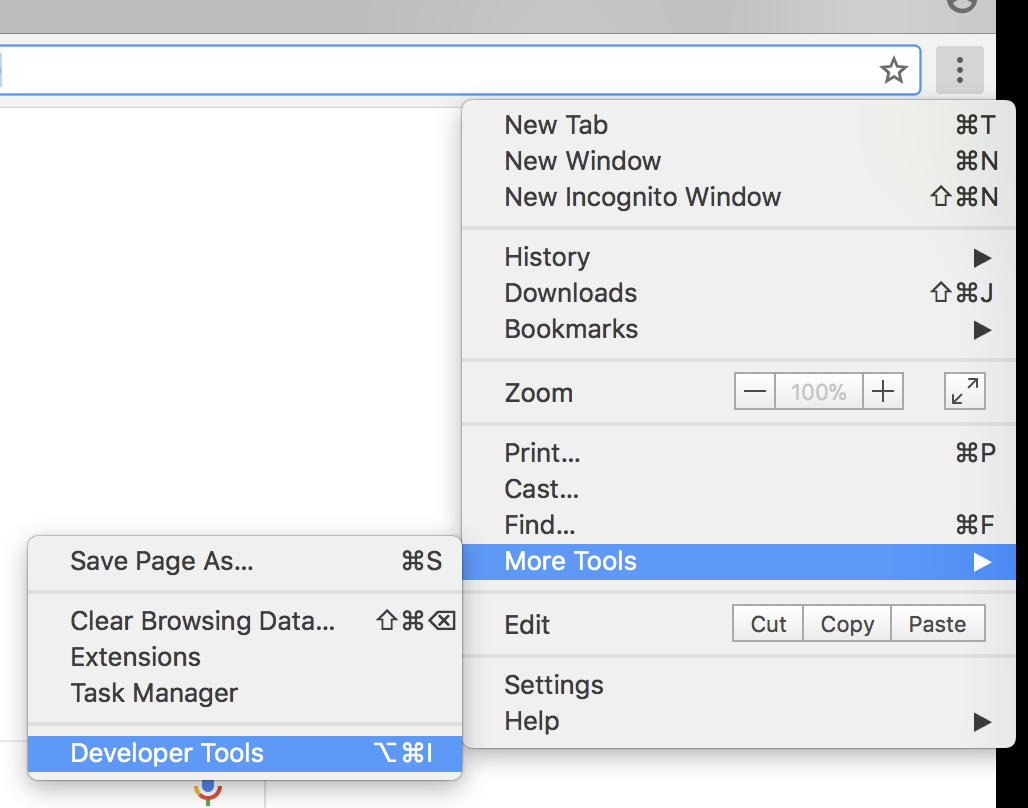
\includegraphics[width=0.8\textwidth]{figures/devtools.png}
\label{fig:devtools}
\end{figure}


\paragraph{} This gives us the following new set of tabs to interact with:

\begin{figure}[H]
\centering

\includegraphics[width=0.8\textwidth]{figures/devtools_toolbar.png}
\label{fig:devtools_toolbar}
\end{figure}


\paragraph{} For each tab we get a different view on aspects of the page that is loaded, for example the "elements" that is the DOM representation of the underlying HTML that the page is made up from. Note that this can become quite complicated because any associated CSS and Javascript can manipulate the HTML elements. As a result the HTML that is rendered in the browser for any given web page that you are viewing can be significantly different to the original HTML source file that was loaded. Remember this, CSS and JS give you great powers to manipulate a page, you can even discard all of the original HTML and completely generate a new replacement page.


\begin{figure}[H]
\centering
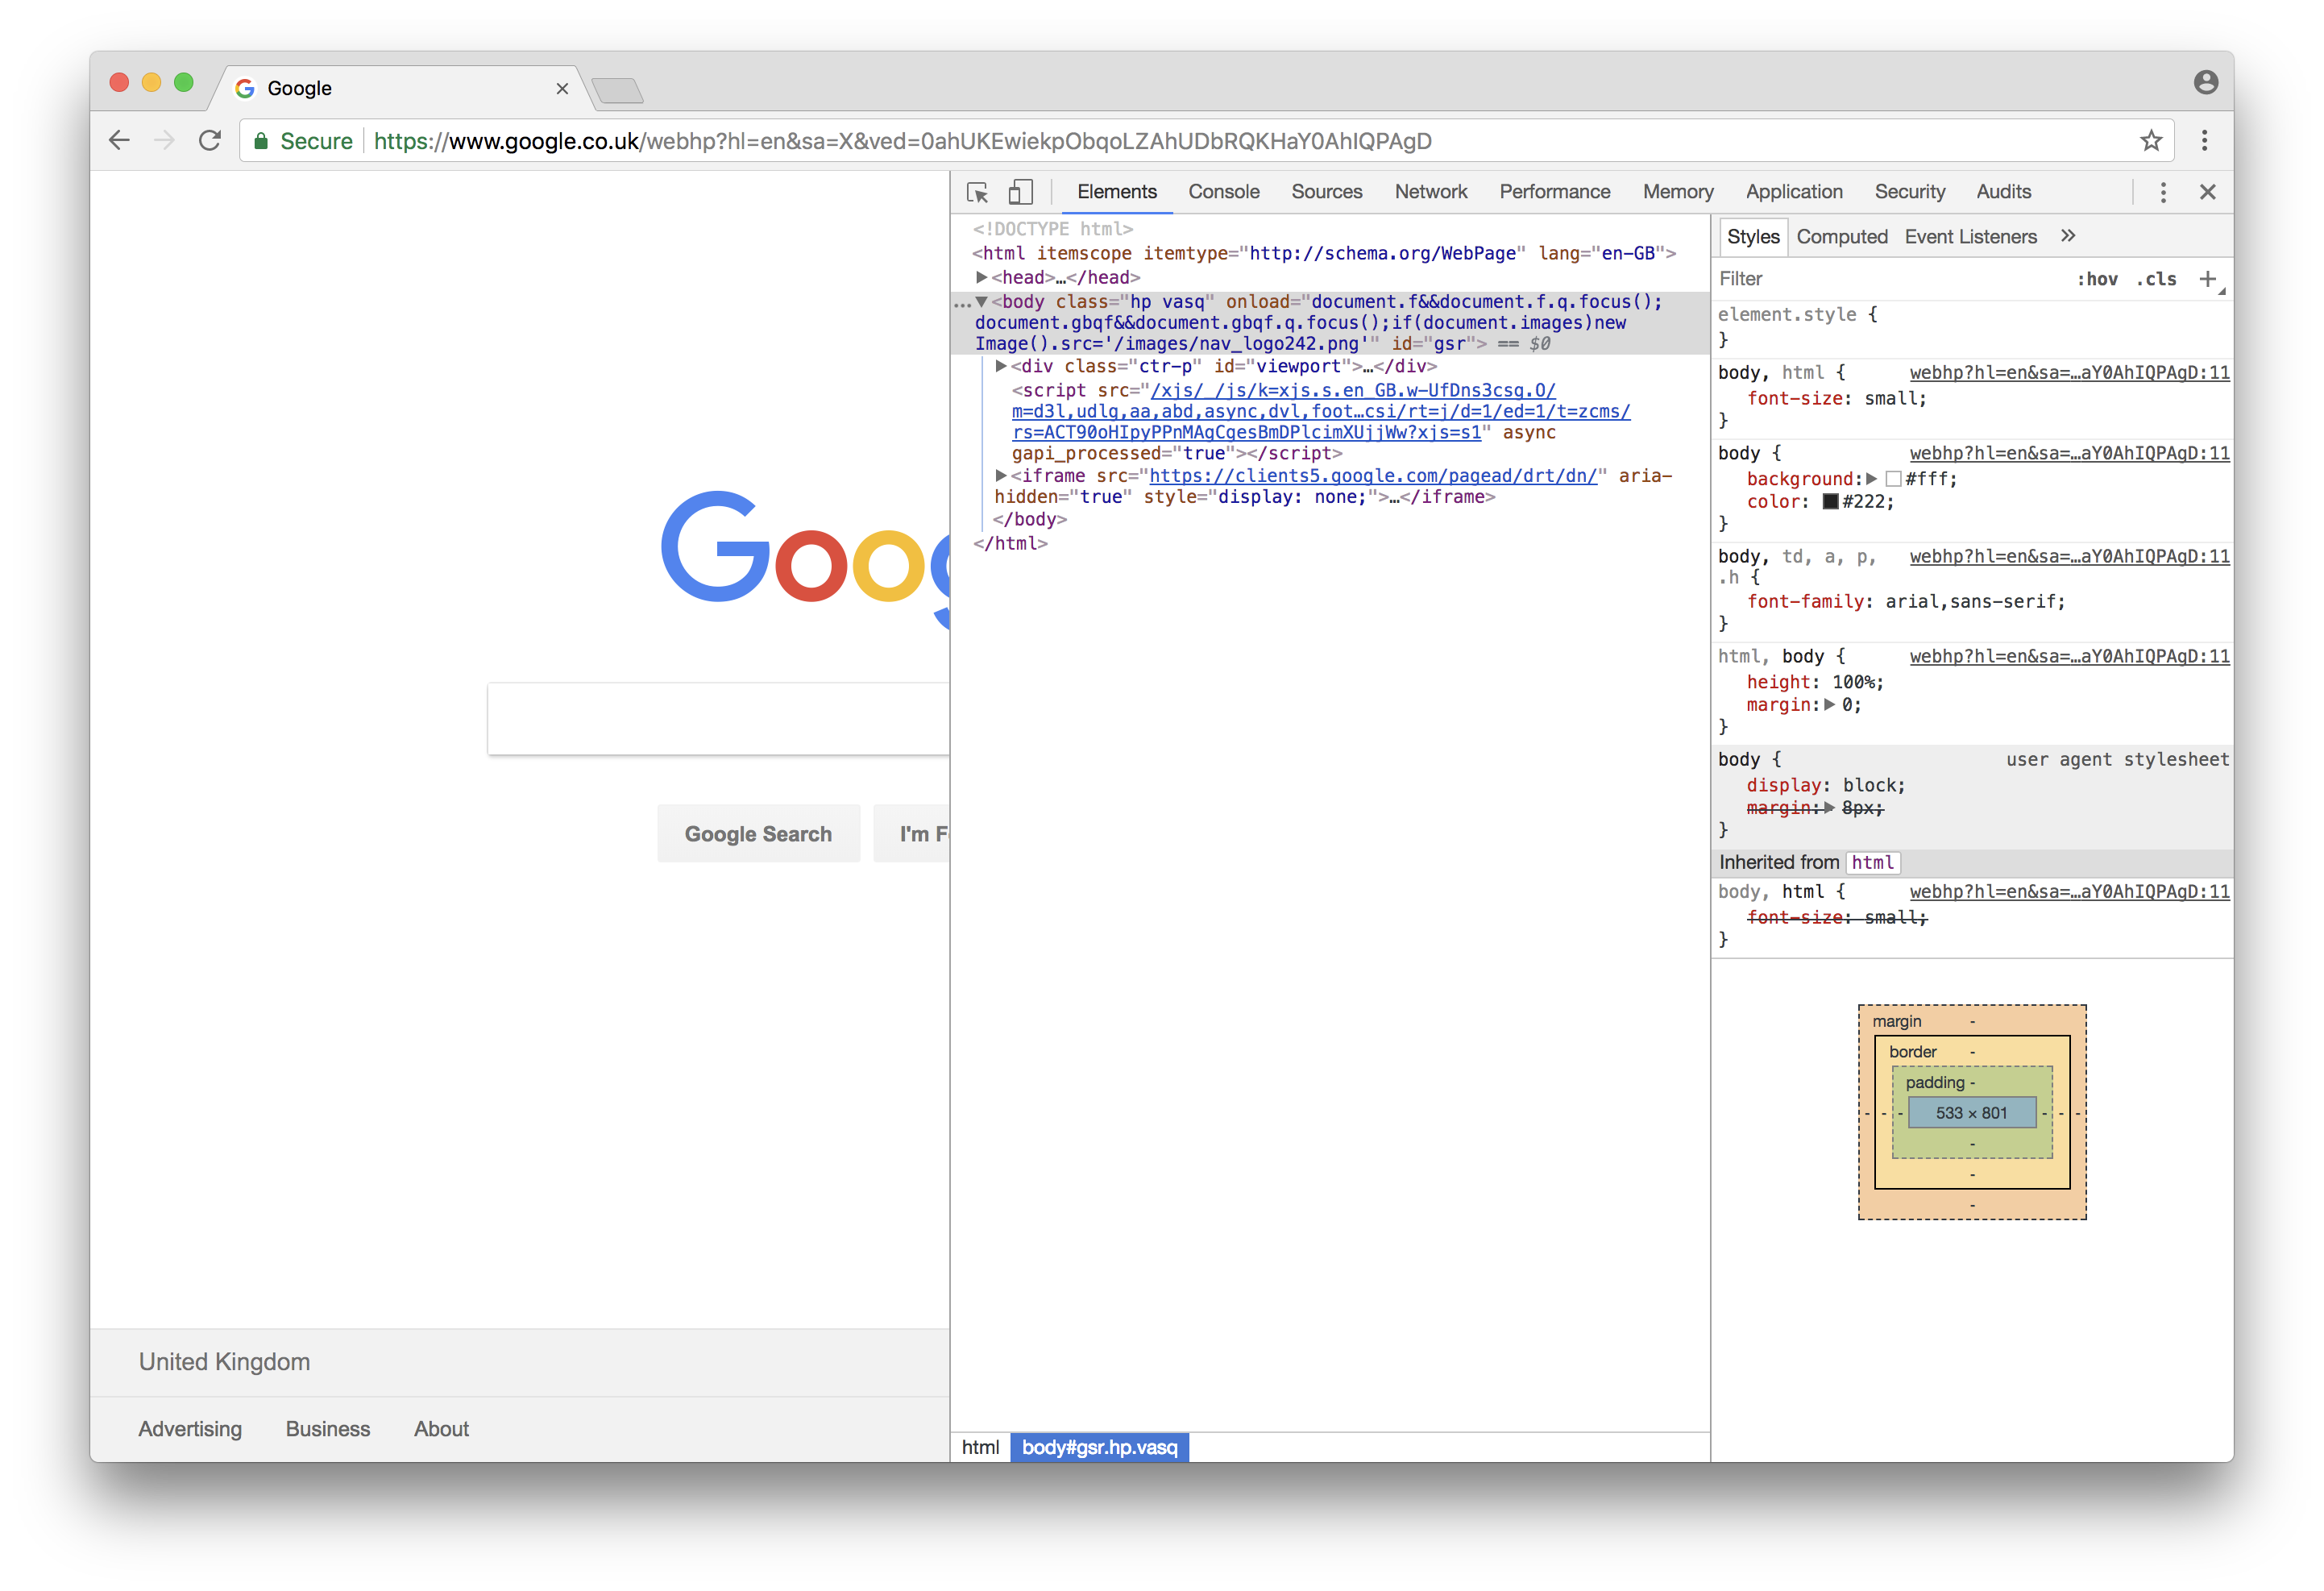
\includegraphics[width=0.8\textwidth]{figures/devtools_elements.png}
\label{fig:devtools_elements}
\end{figure}

\paragraph{} The next tab is for the console. This is a place that you will need to look at frequently as you develop your sites as it is the location where errors, warnings, and messages are printed when things go wrong.  You can also use it as a location to execute your own javascript. Just open the console and write some code then when you press return it will be executed. When you write more extensive JS in subsequent units you will find the console is a useful and important tool to have ready in your toolbox.


\begin{figure}[H]
\centering
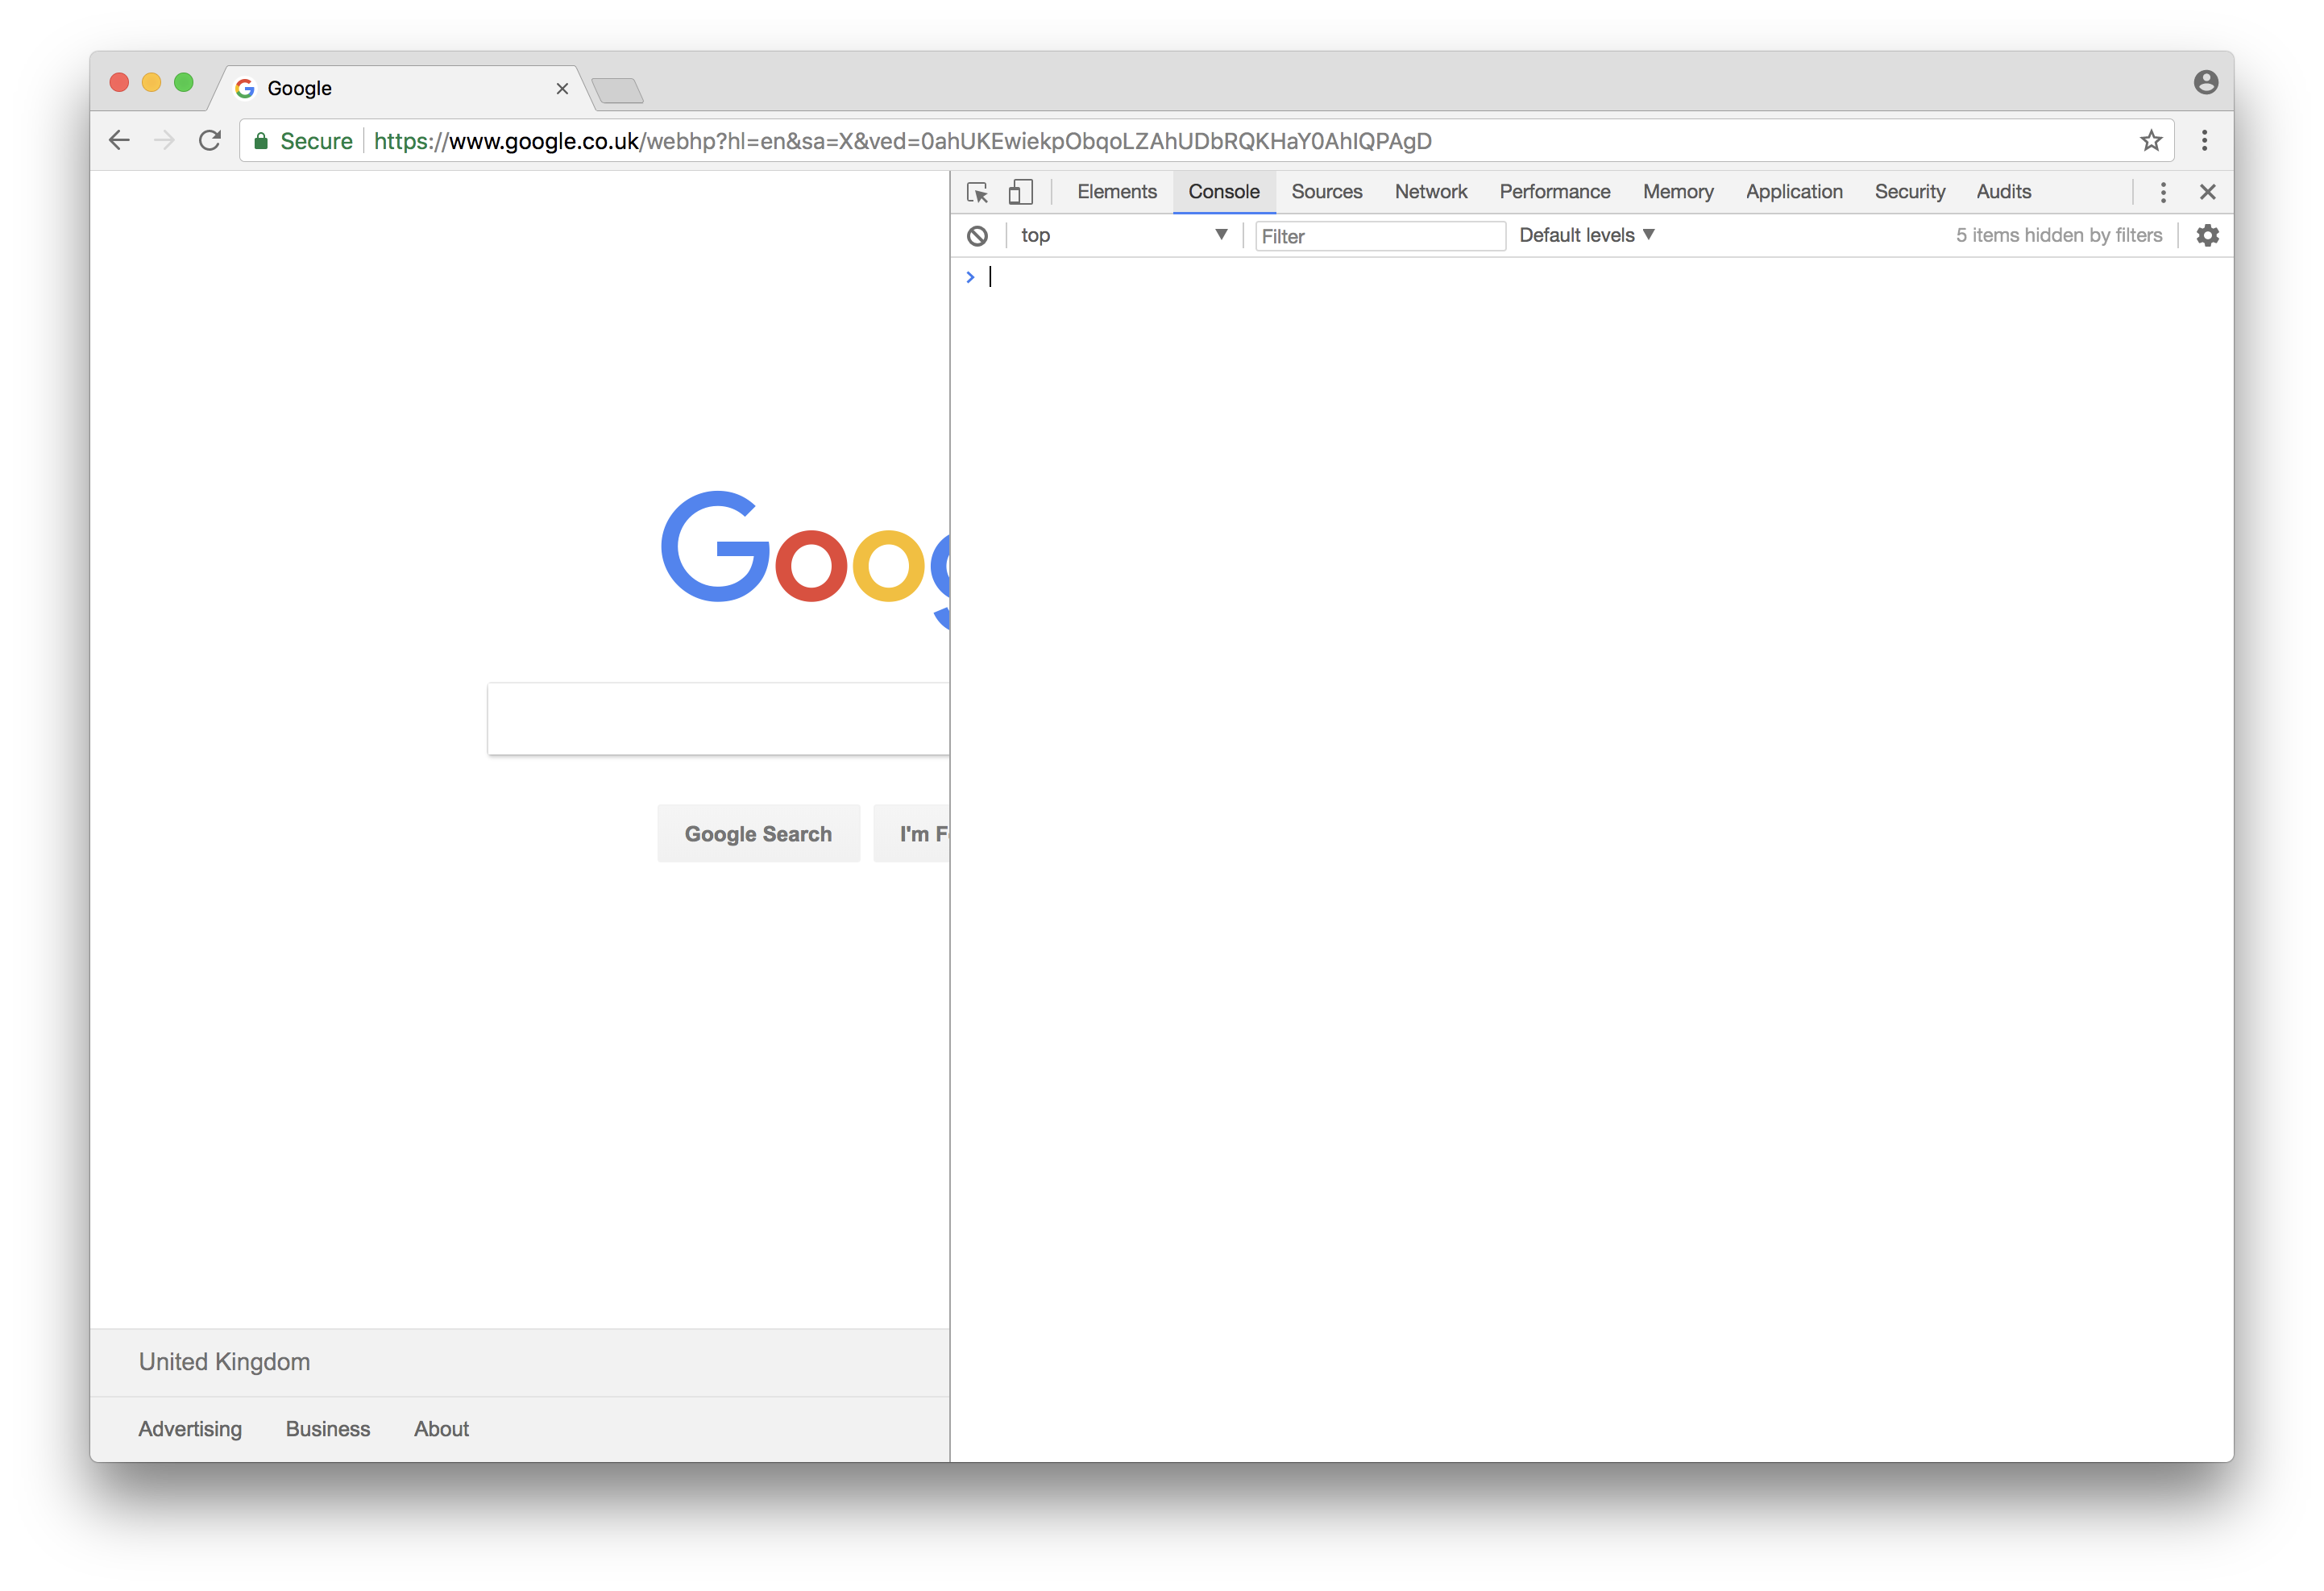
\includegraphics[width=0.8\textwidth]{figures/devtools_console.png}
\label{fig:devtools_console}
\end{figure}


\paragraph{} Next is the sources tab which will come in useful when we are dealing with deployed sites as it gives us a way to track all of the different resources that our pages use:


\begin{figure}[H]
\centering
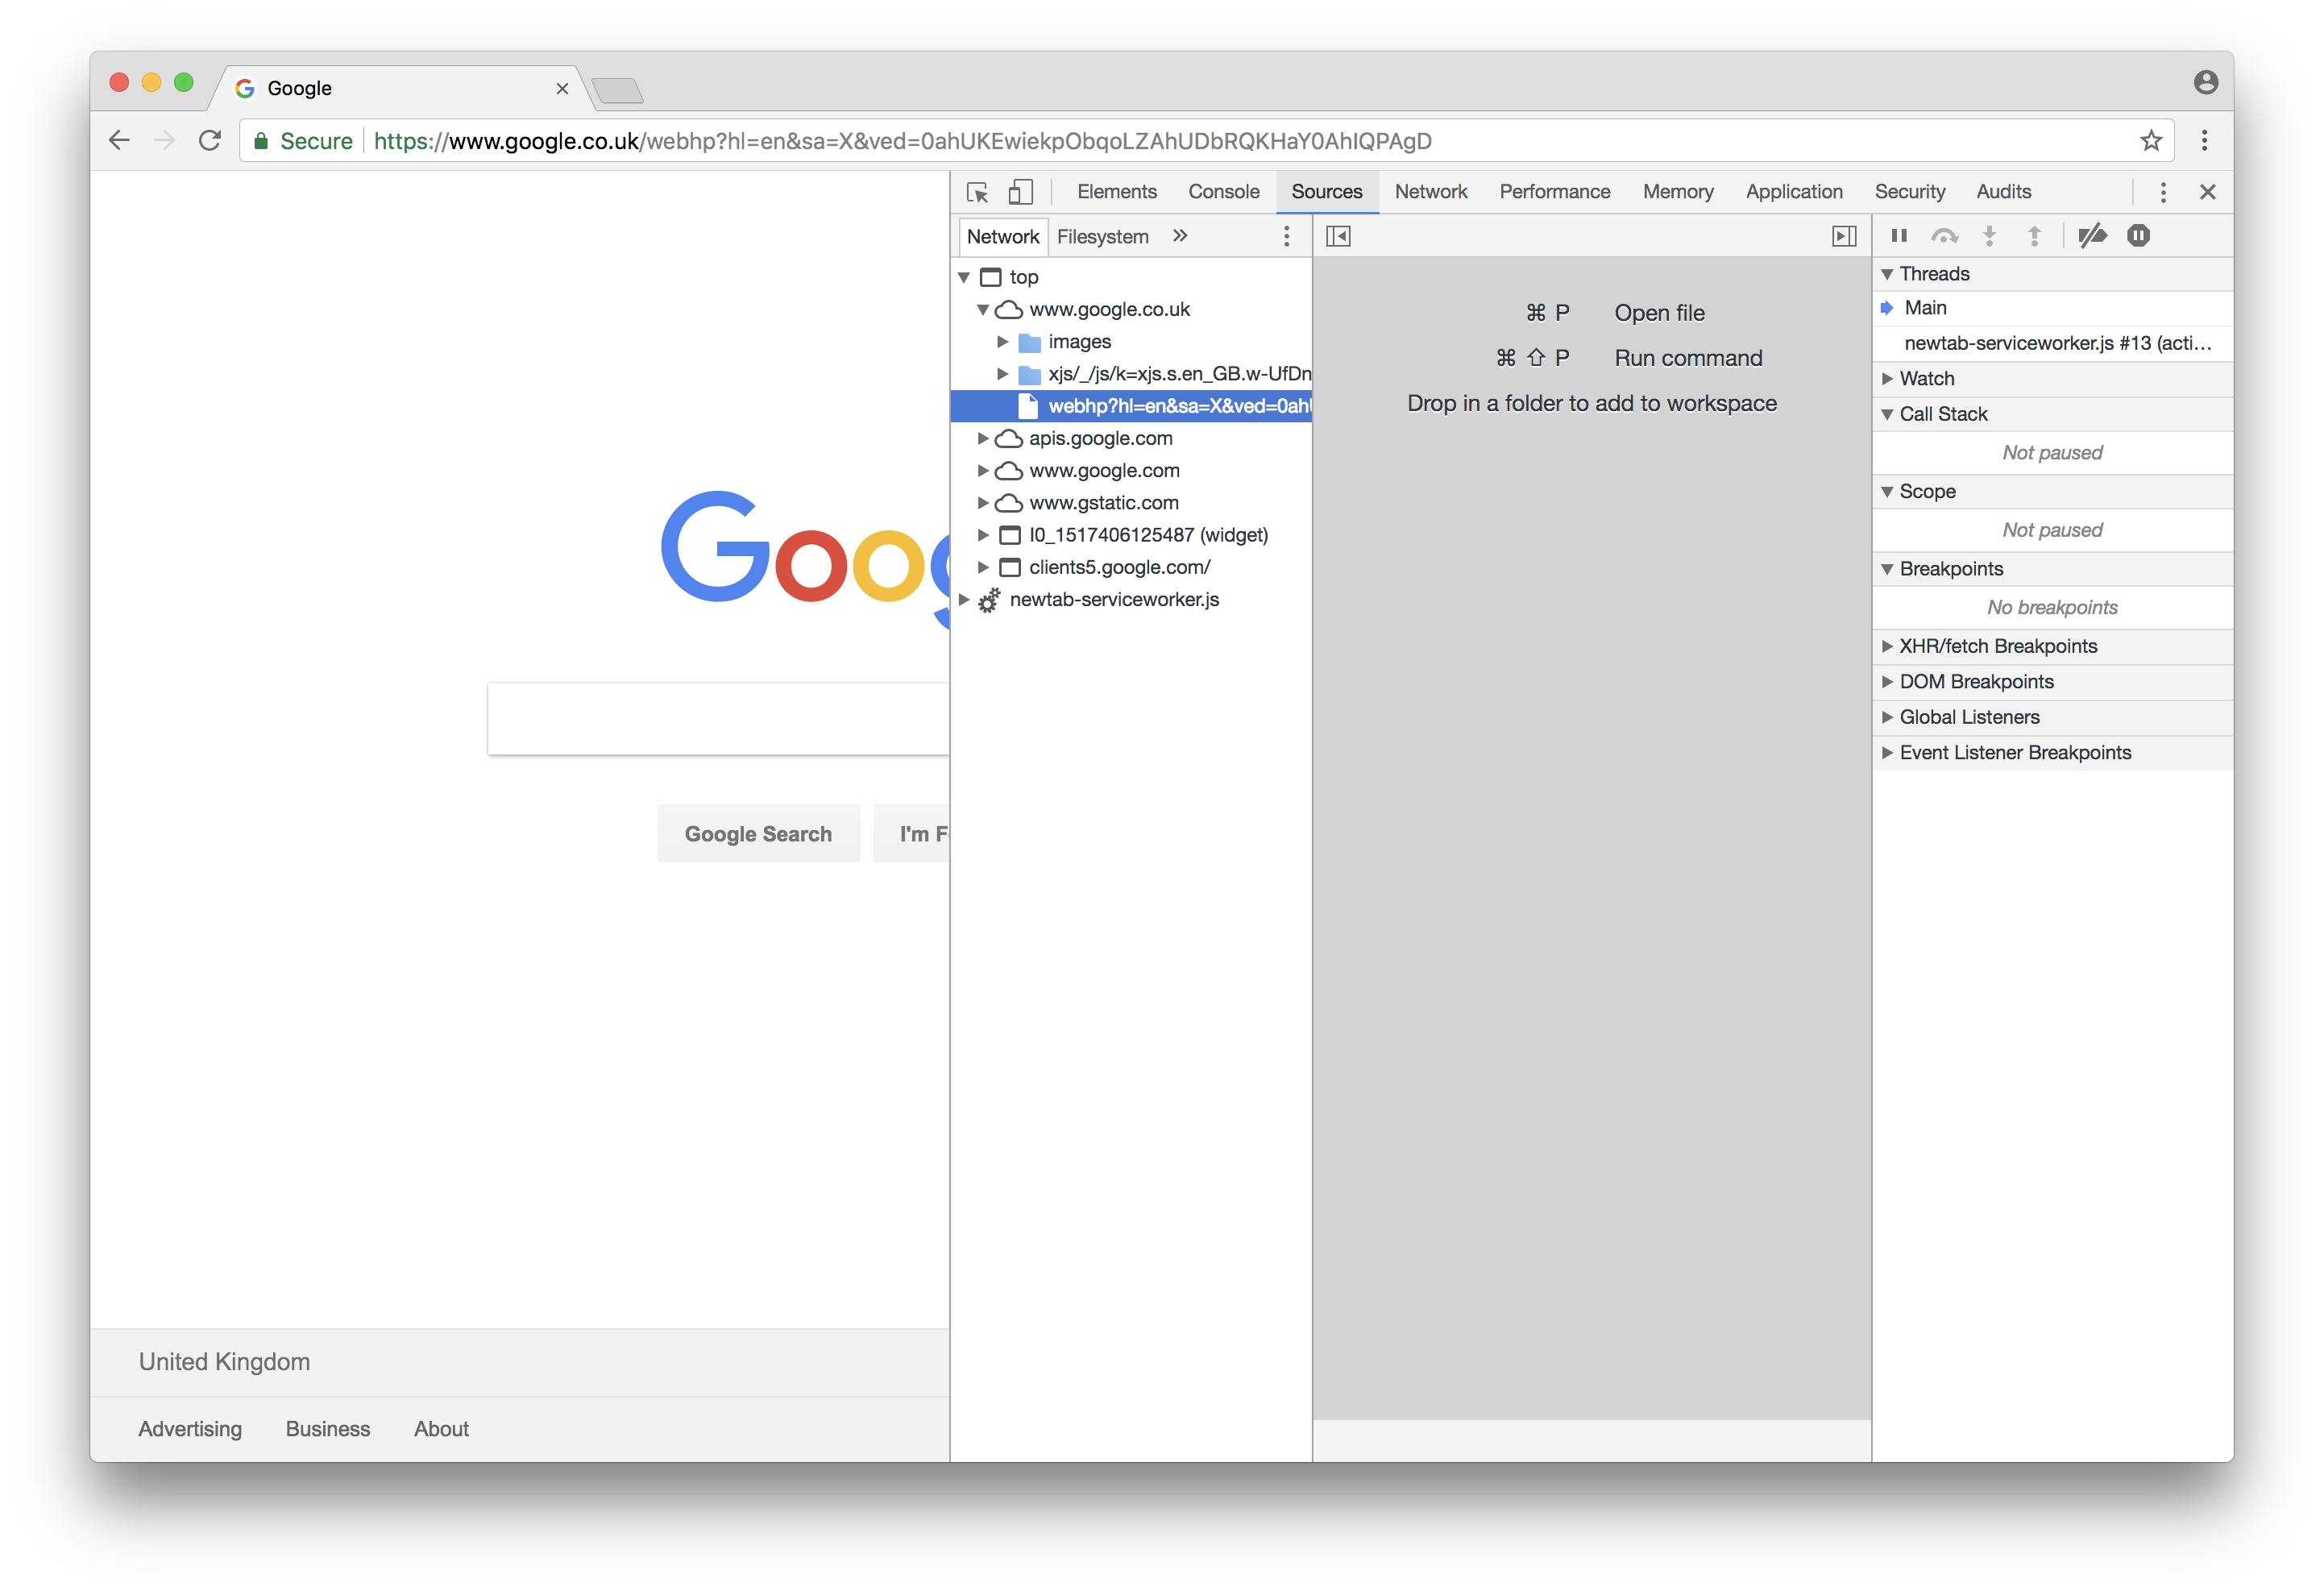
\includegraphics[width=0.8\textwidth]{figures/devtools_sources.png}
\label{fig:devtools_sources}
\end{figure}

\paragraph{} Our next tab, the network tab, gives us information about data and files being moved over the network/Internet/Web between your browser tab and all of the resources that the current web page is built from. This can be very useful when we build more complicated pages and need to debug why something isn't quite right.

\begin{figure}[H]
\centering
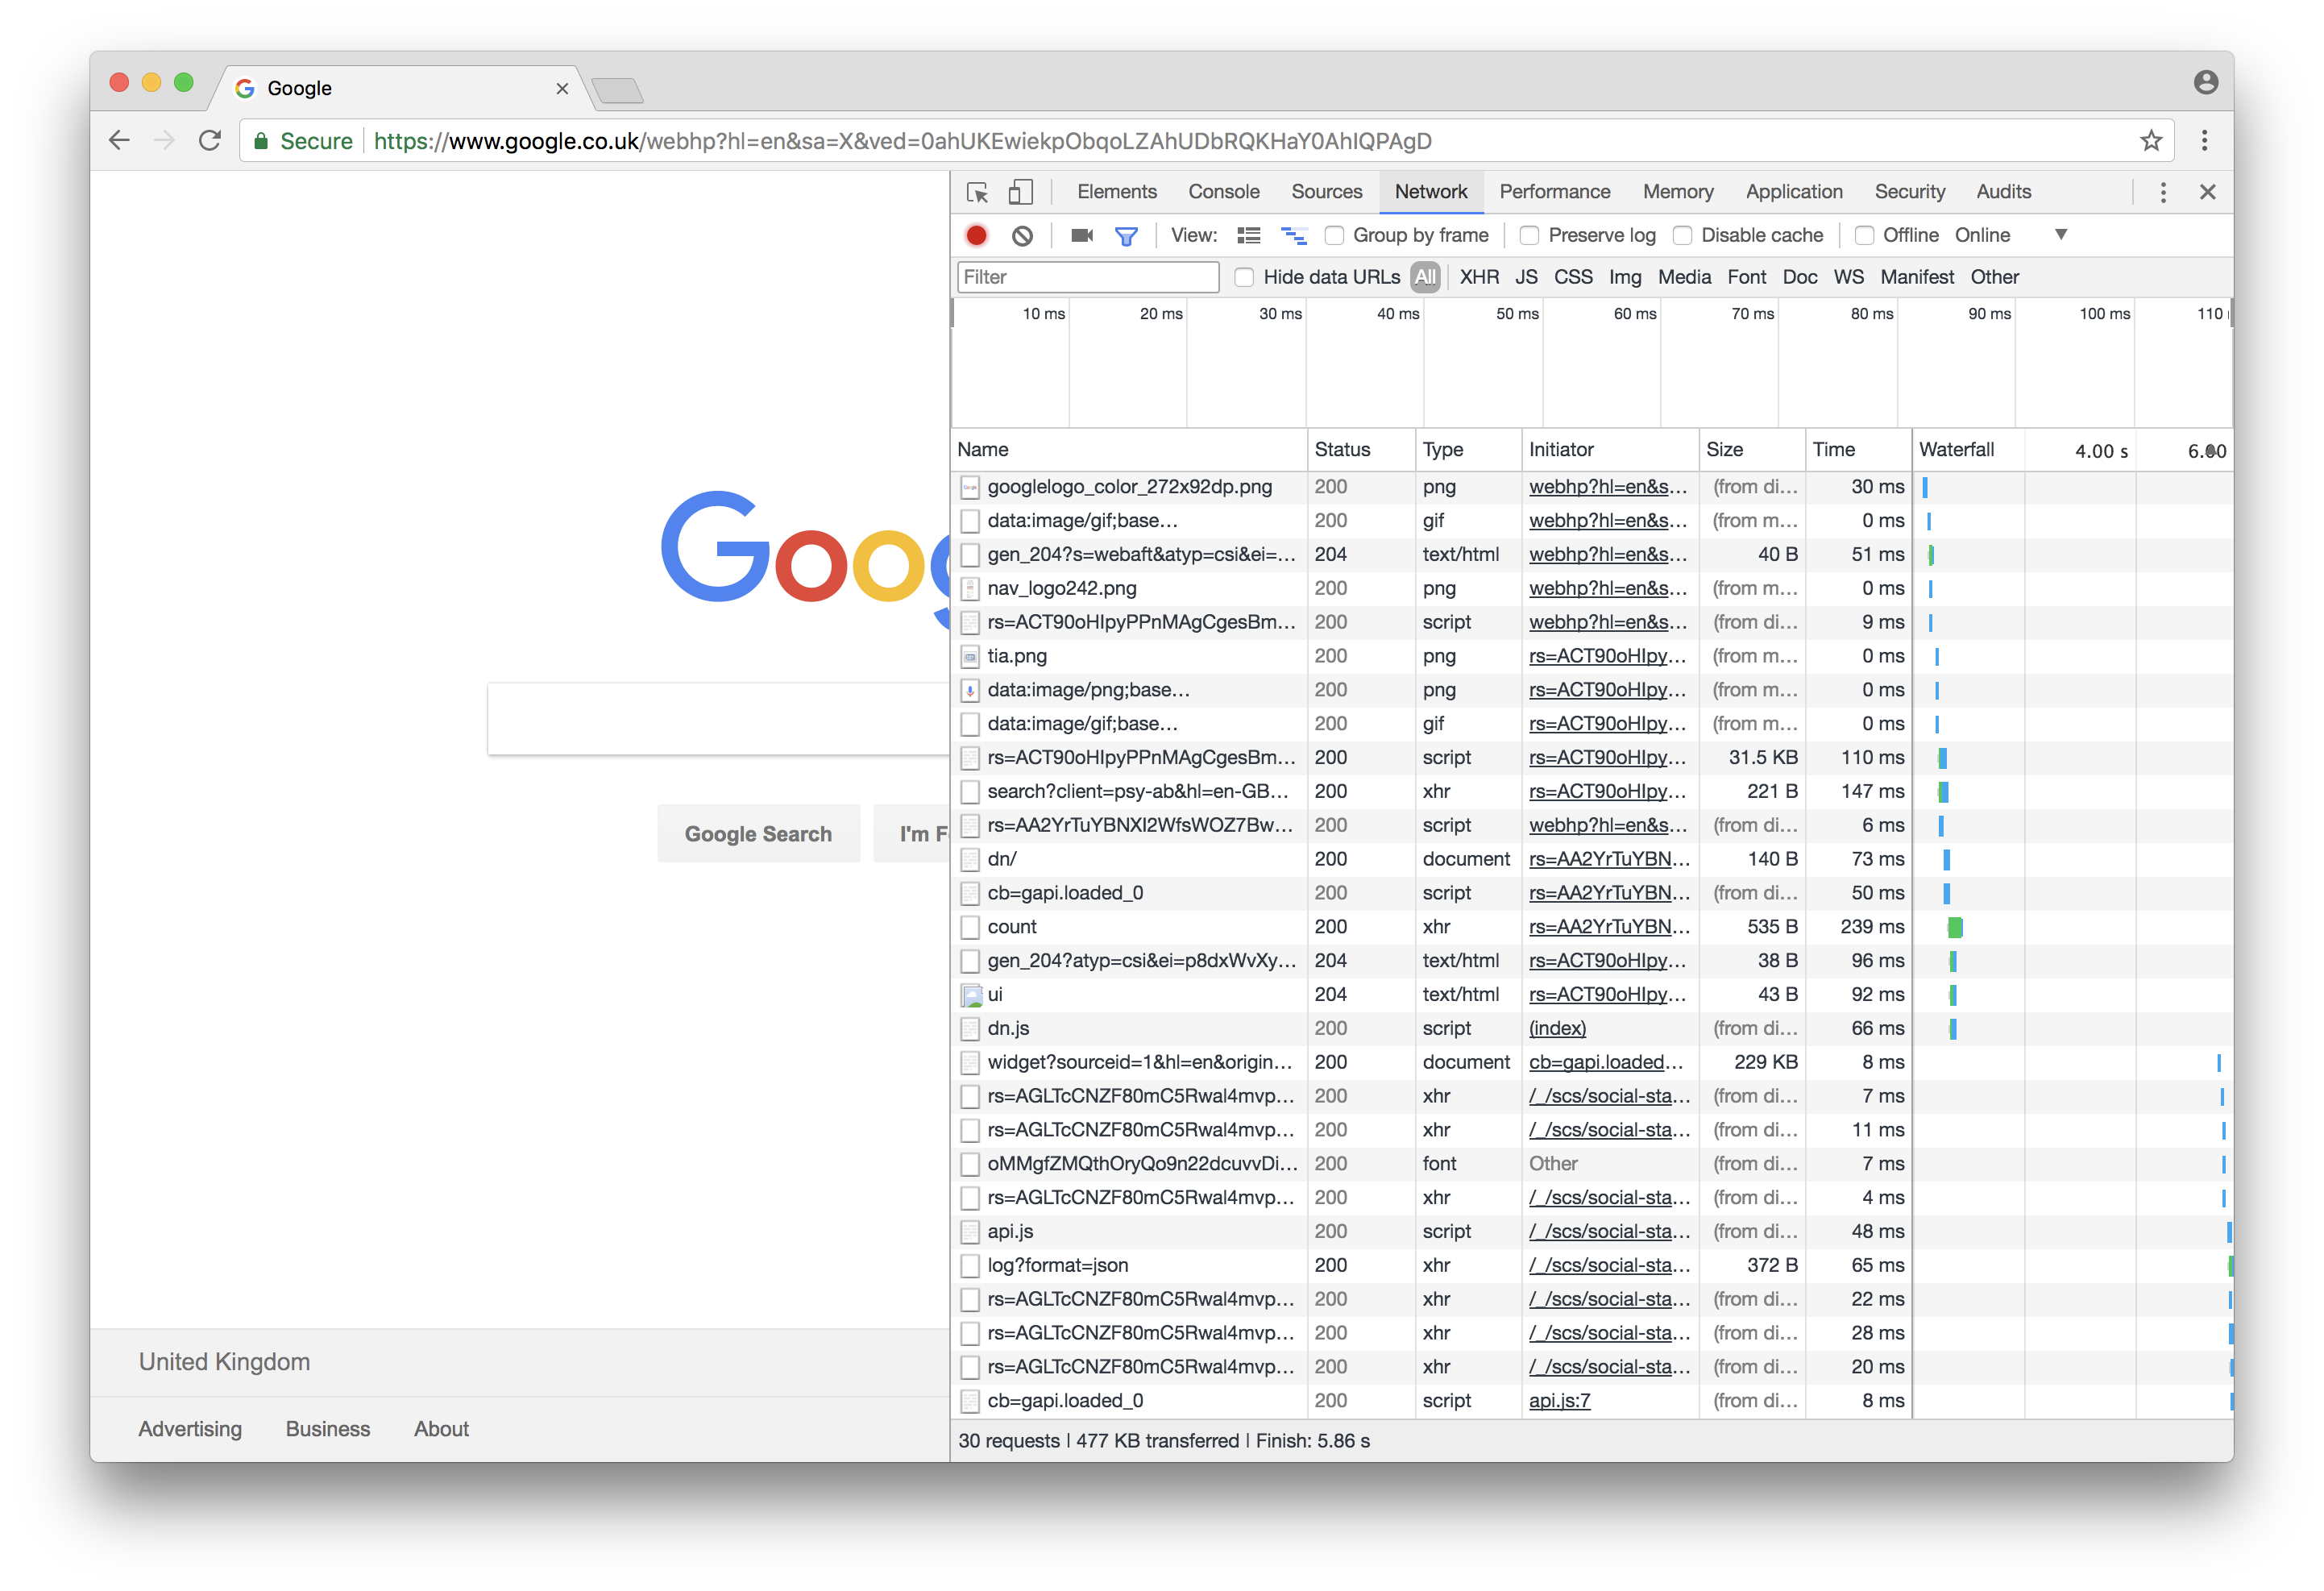
\includegraphics[width=0.8\textwidth]{figures/devtools-network.png}
\label{fig:devtools-network}
\end{figure}


\paragraph{} Next we have the performance monitor which we can use to inspect how well a page is working:

\begin{figure}[H]
\centering
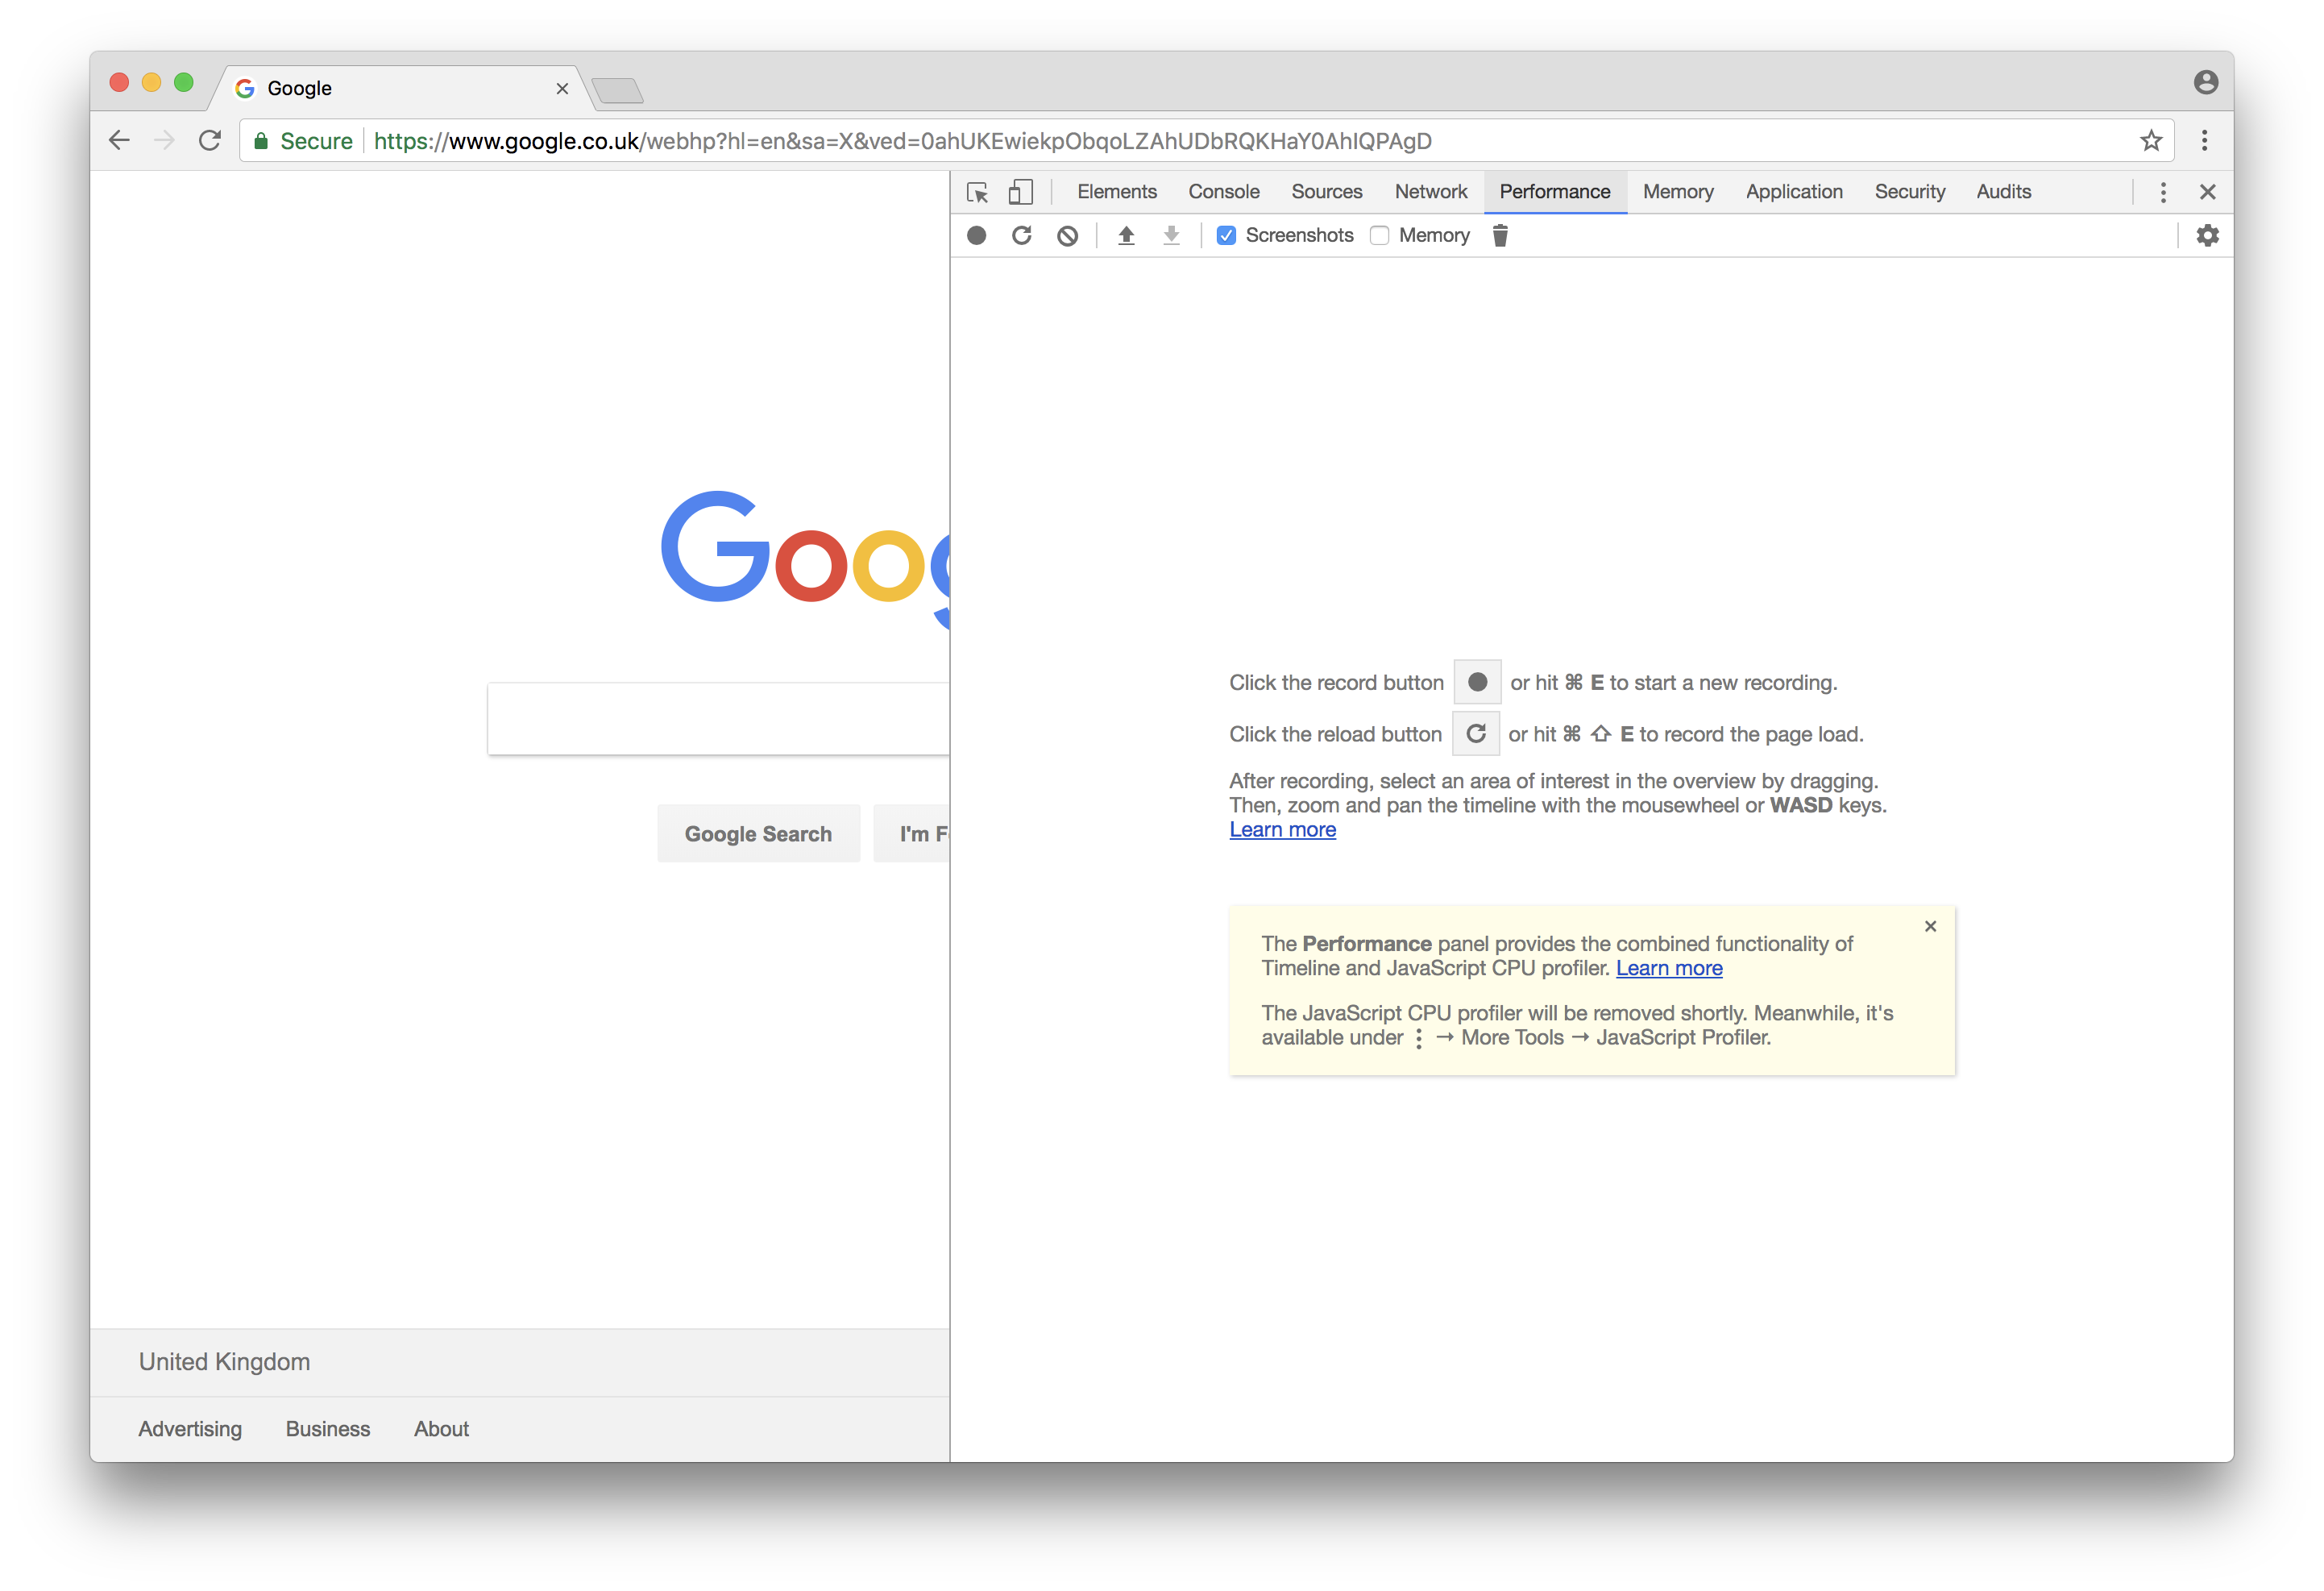
\includegraphics[width=0.8\textwidth]{figures/devtools-performance.png}
\label{fig:devtools-performance}
\end{figure}

\paragraph{} We can also profile memory usage which can be useful as start to write more extensive Javascript:

\begin{figure}[H]
\centering
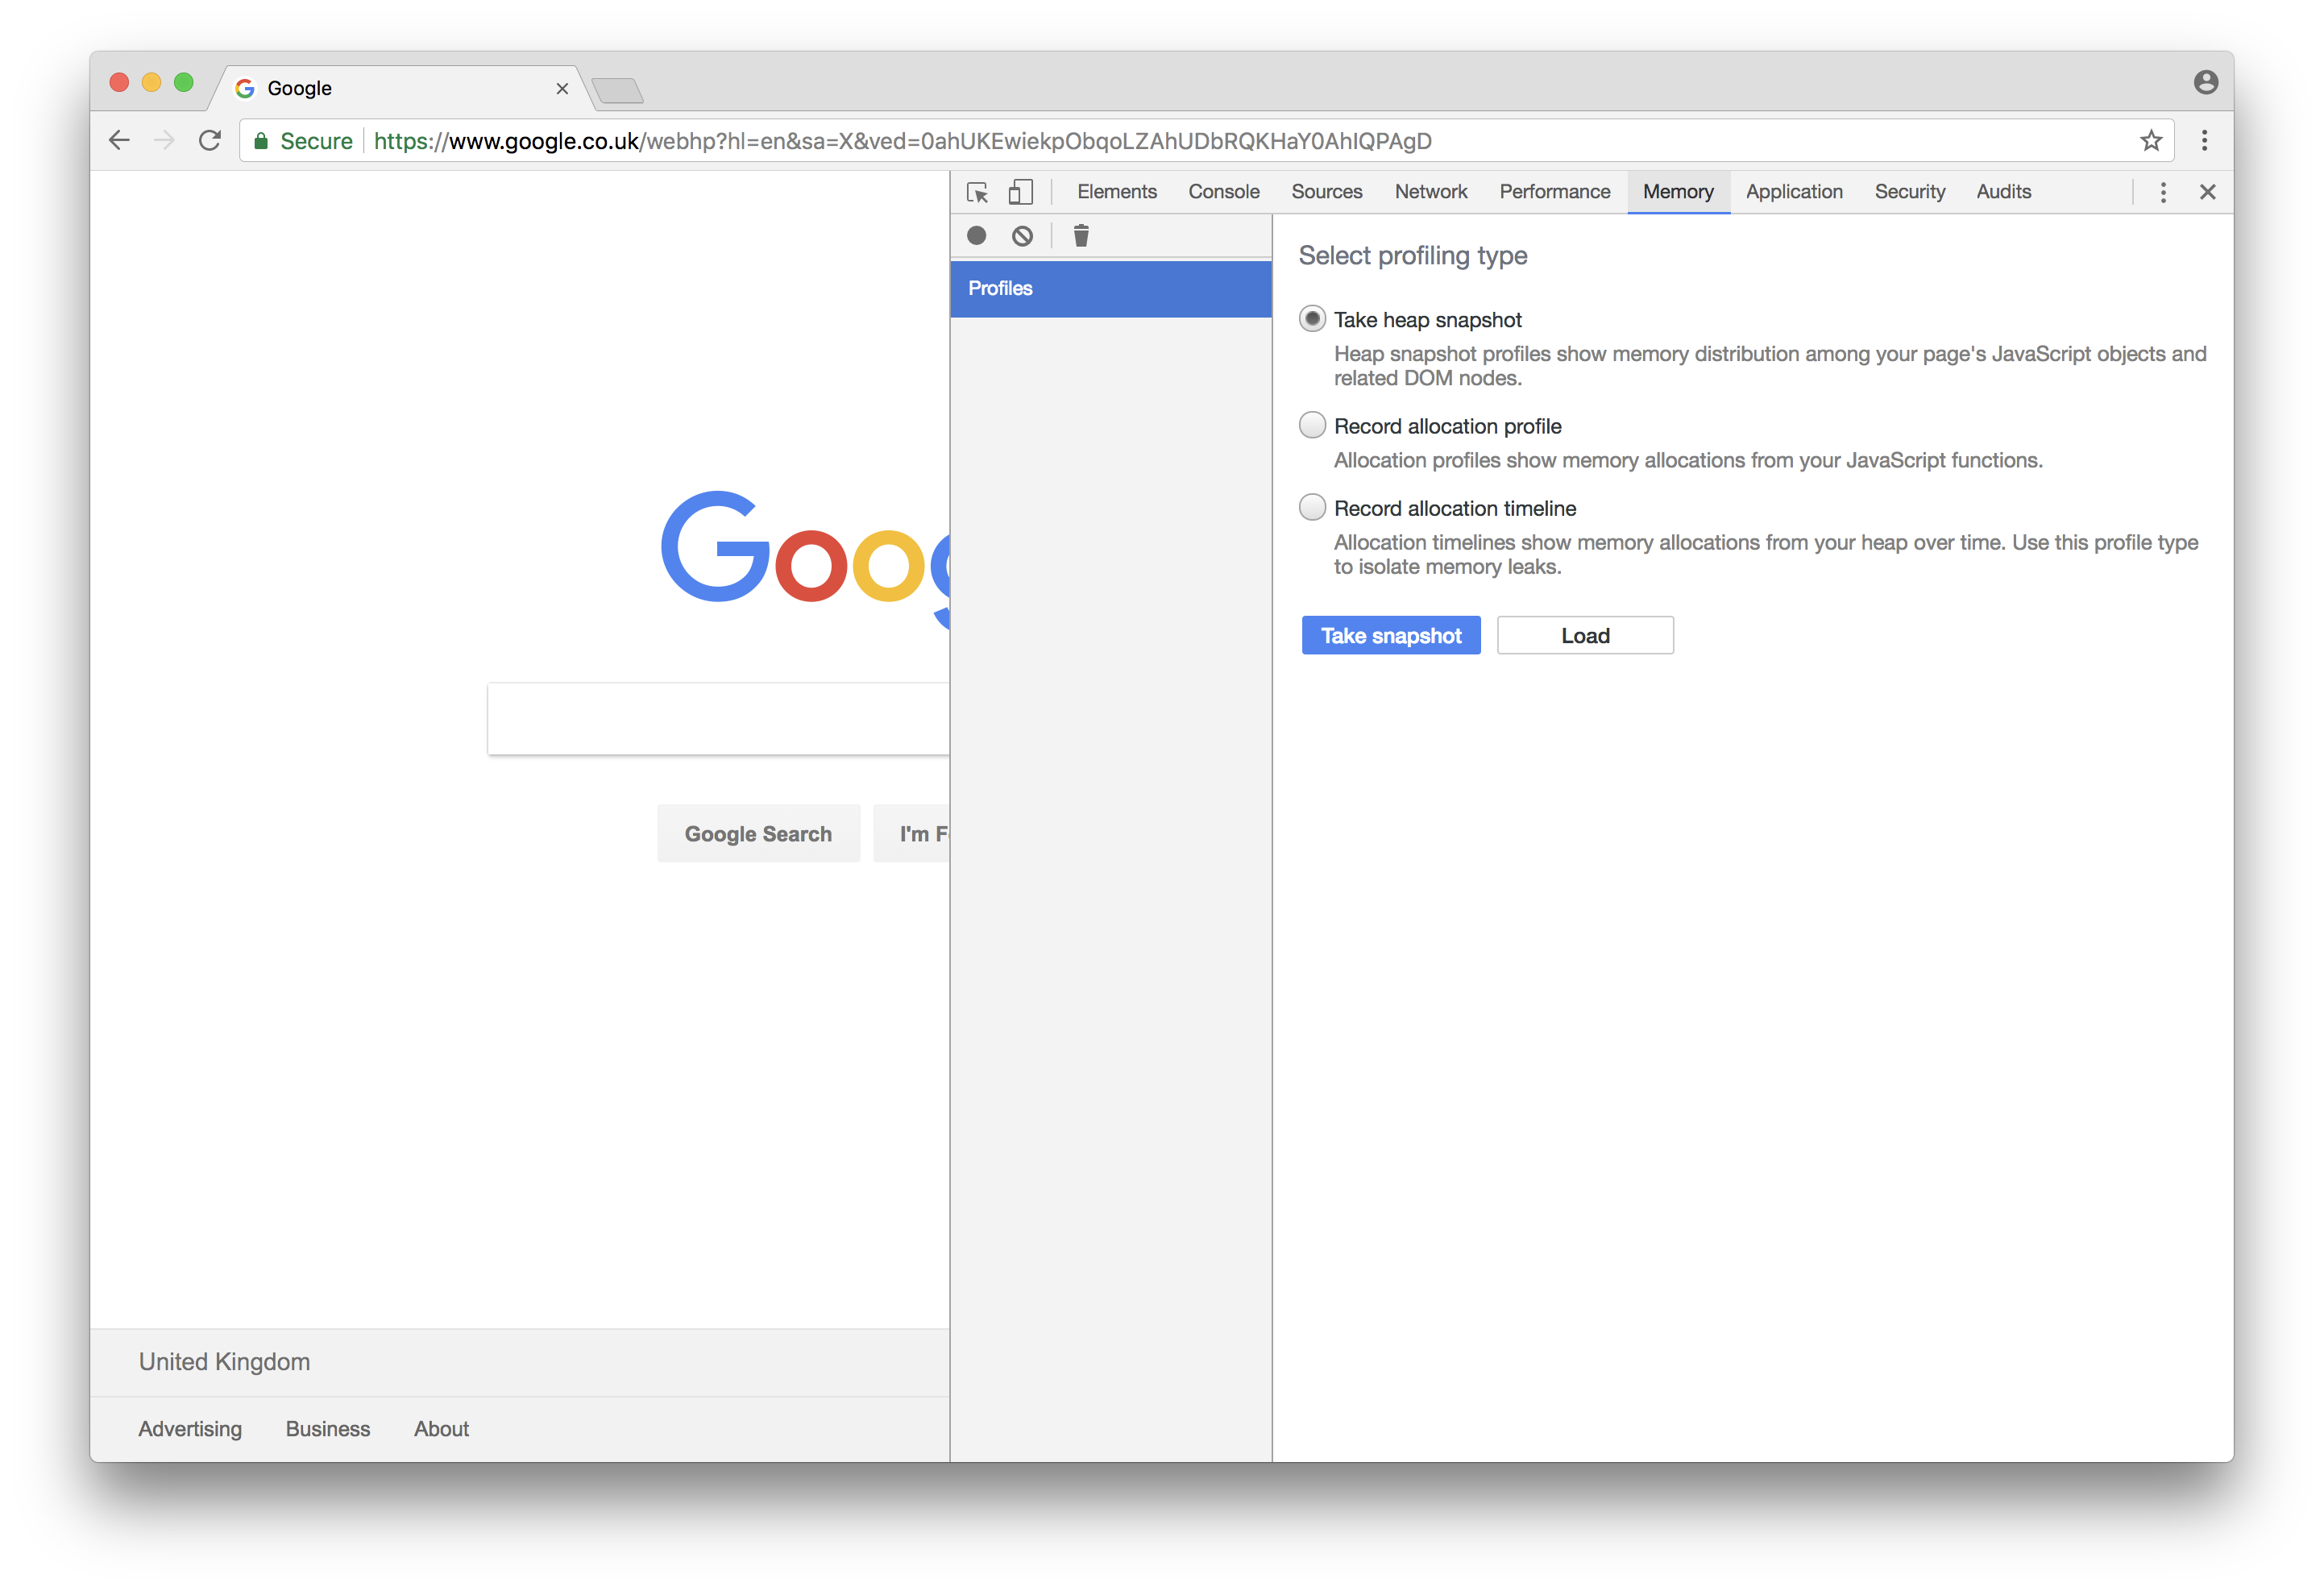
\includegraphics[width=0.8\textwidth]{figures/devtools-memory.png}
\label{fig:devtools-memory}
\end{figure}


\paragraph{} We can inspect aspects of the current web application, e.g. how local storage is being used, and which information is being cached:

\begin{figure}[H]
\centering
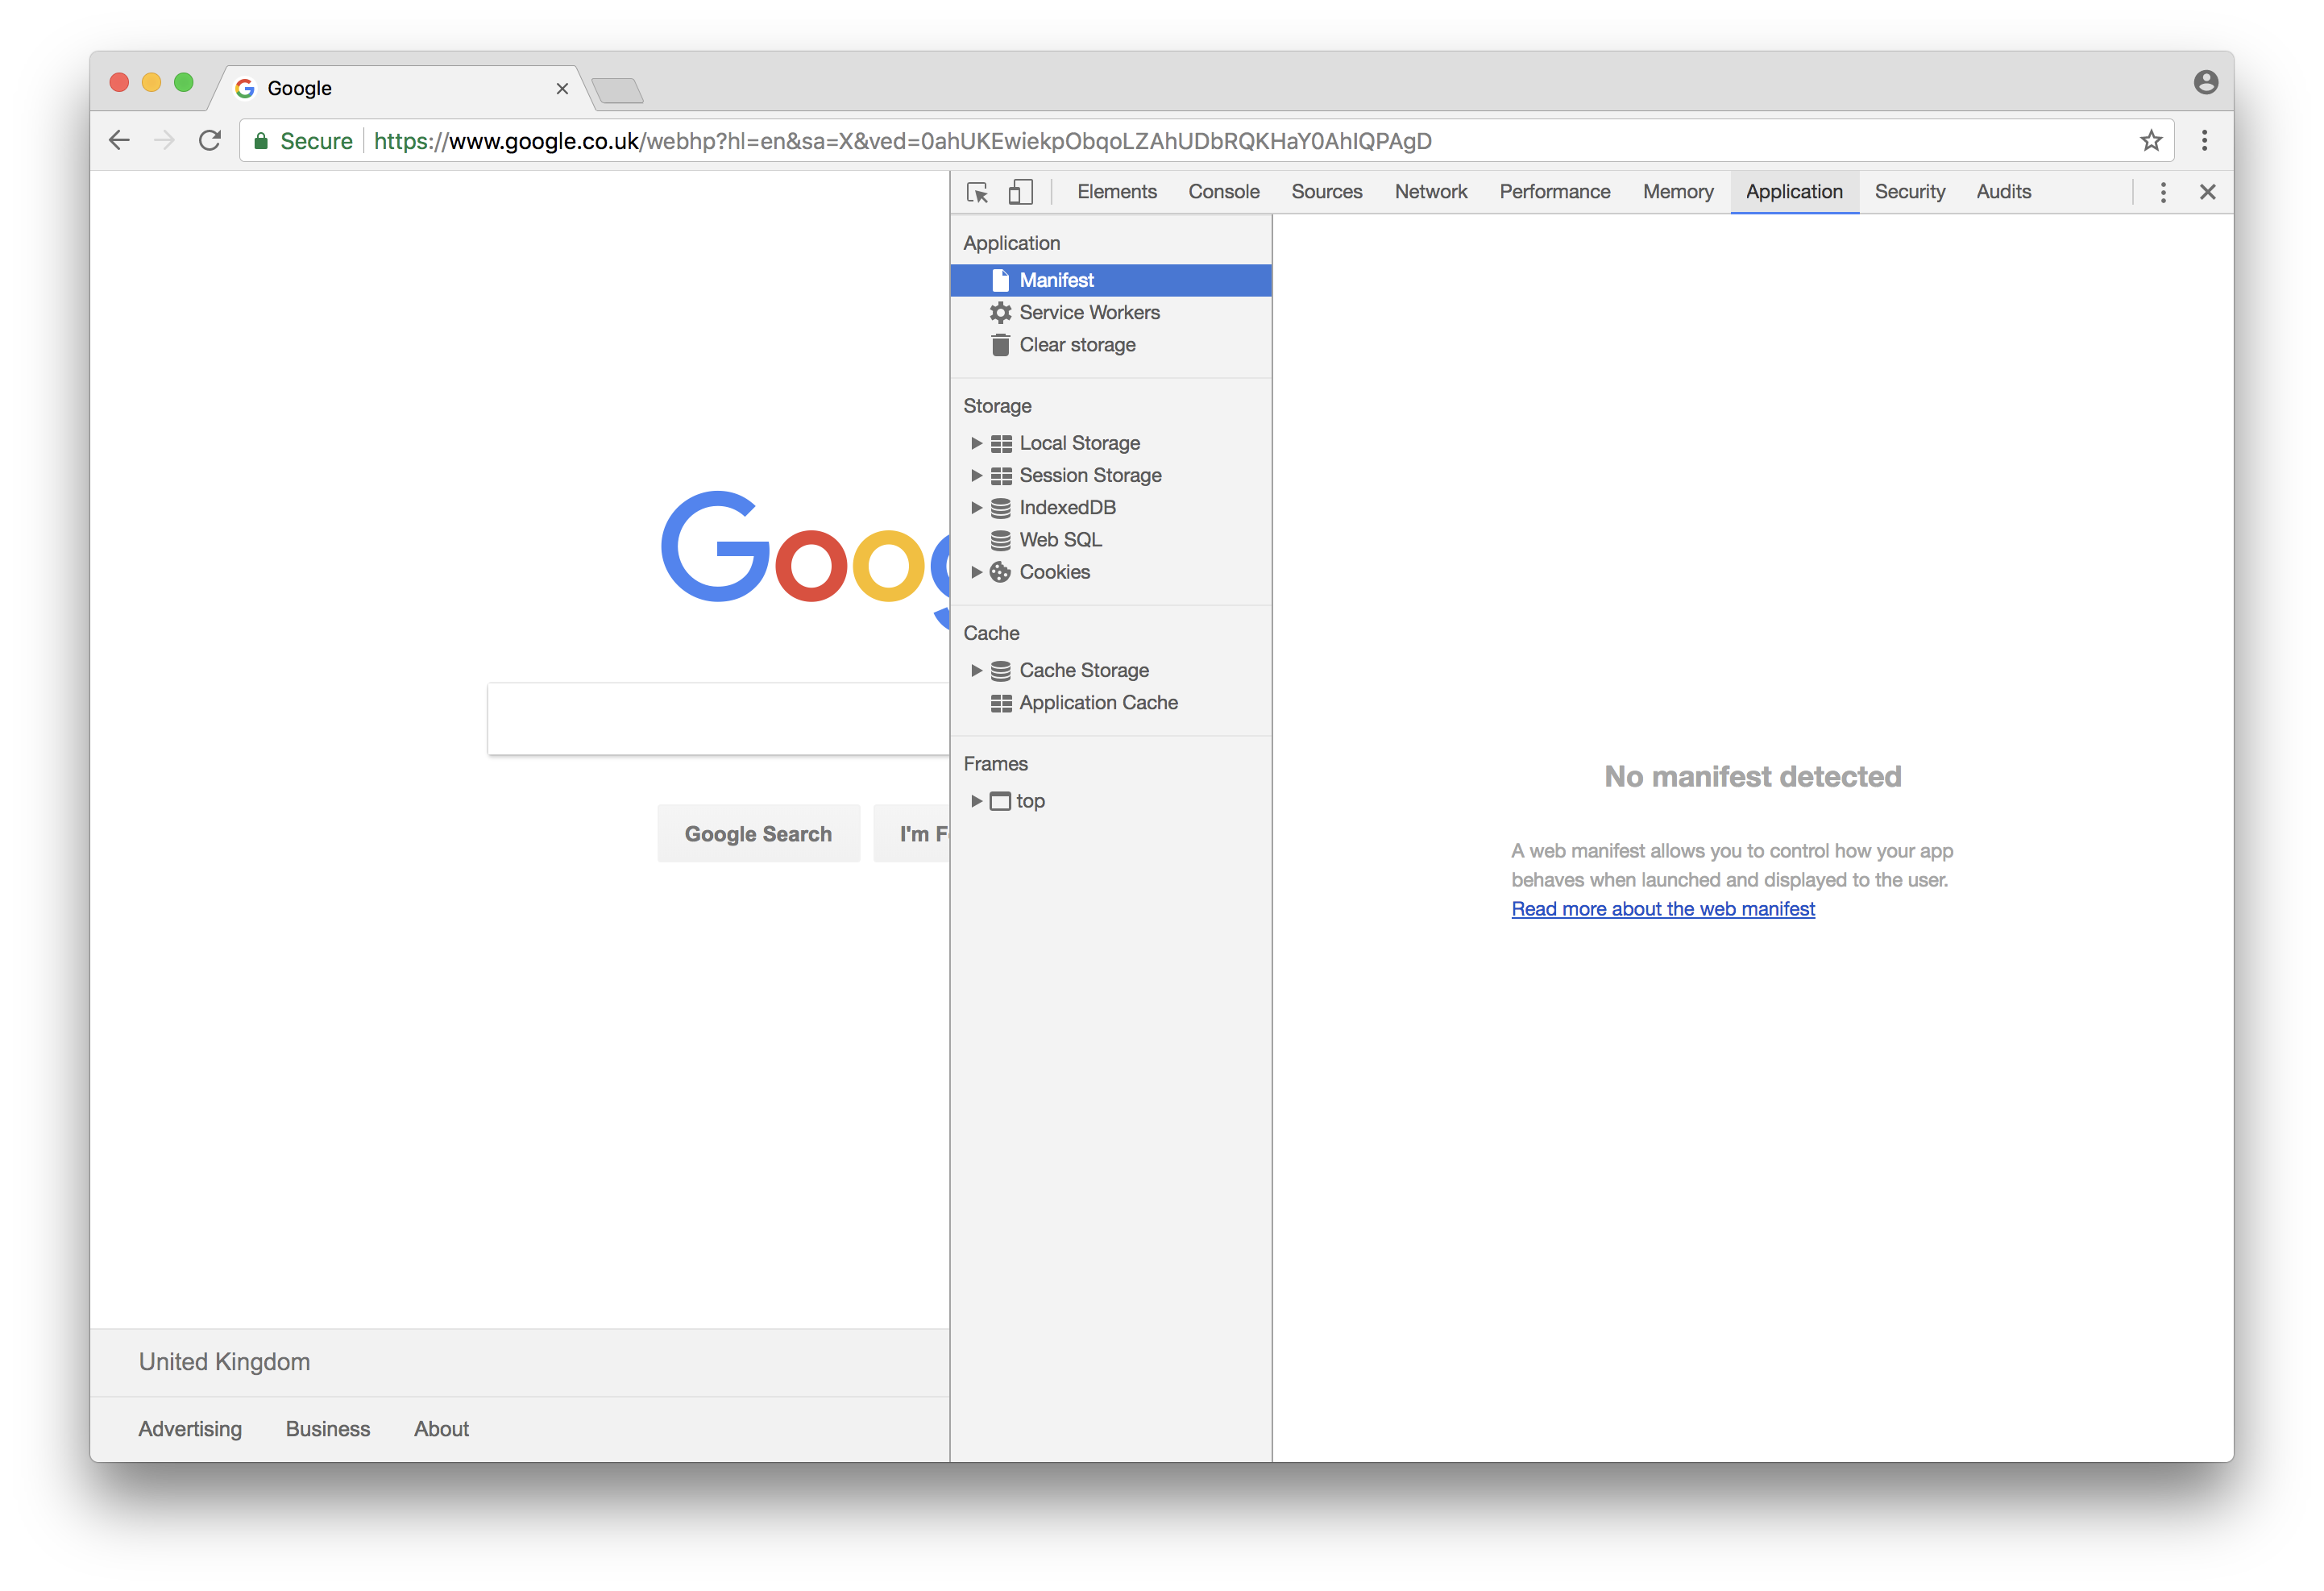
\includegraphics[width=0.8\textwidth]{figures/devtools-application.png}
\label{fig:devtools-application}
\end{figure}


\paragraph{} We can also inspect browser related security features:

\begin{figure}[H]
\centering
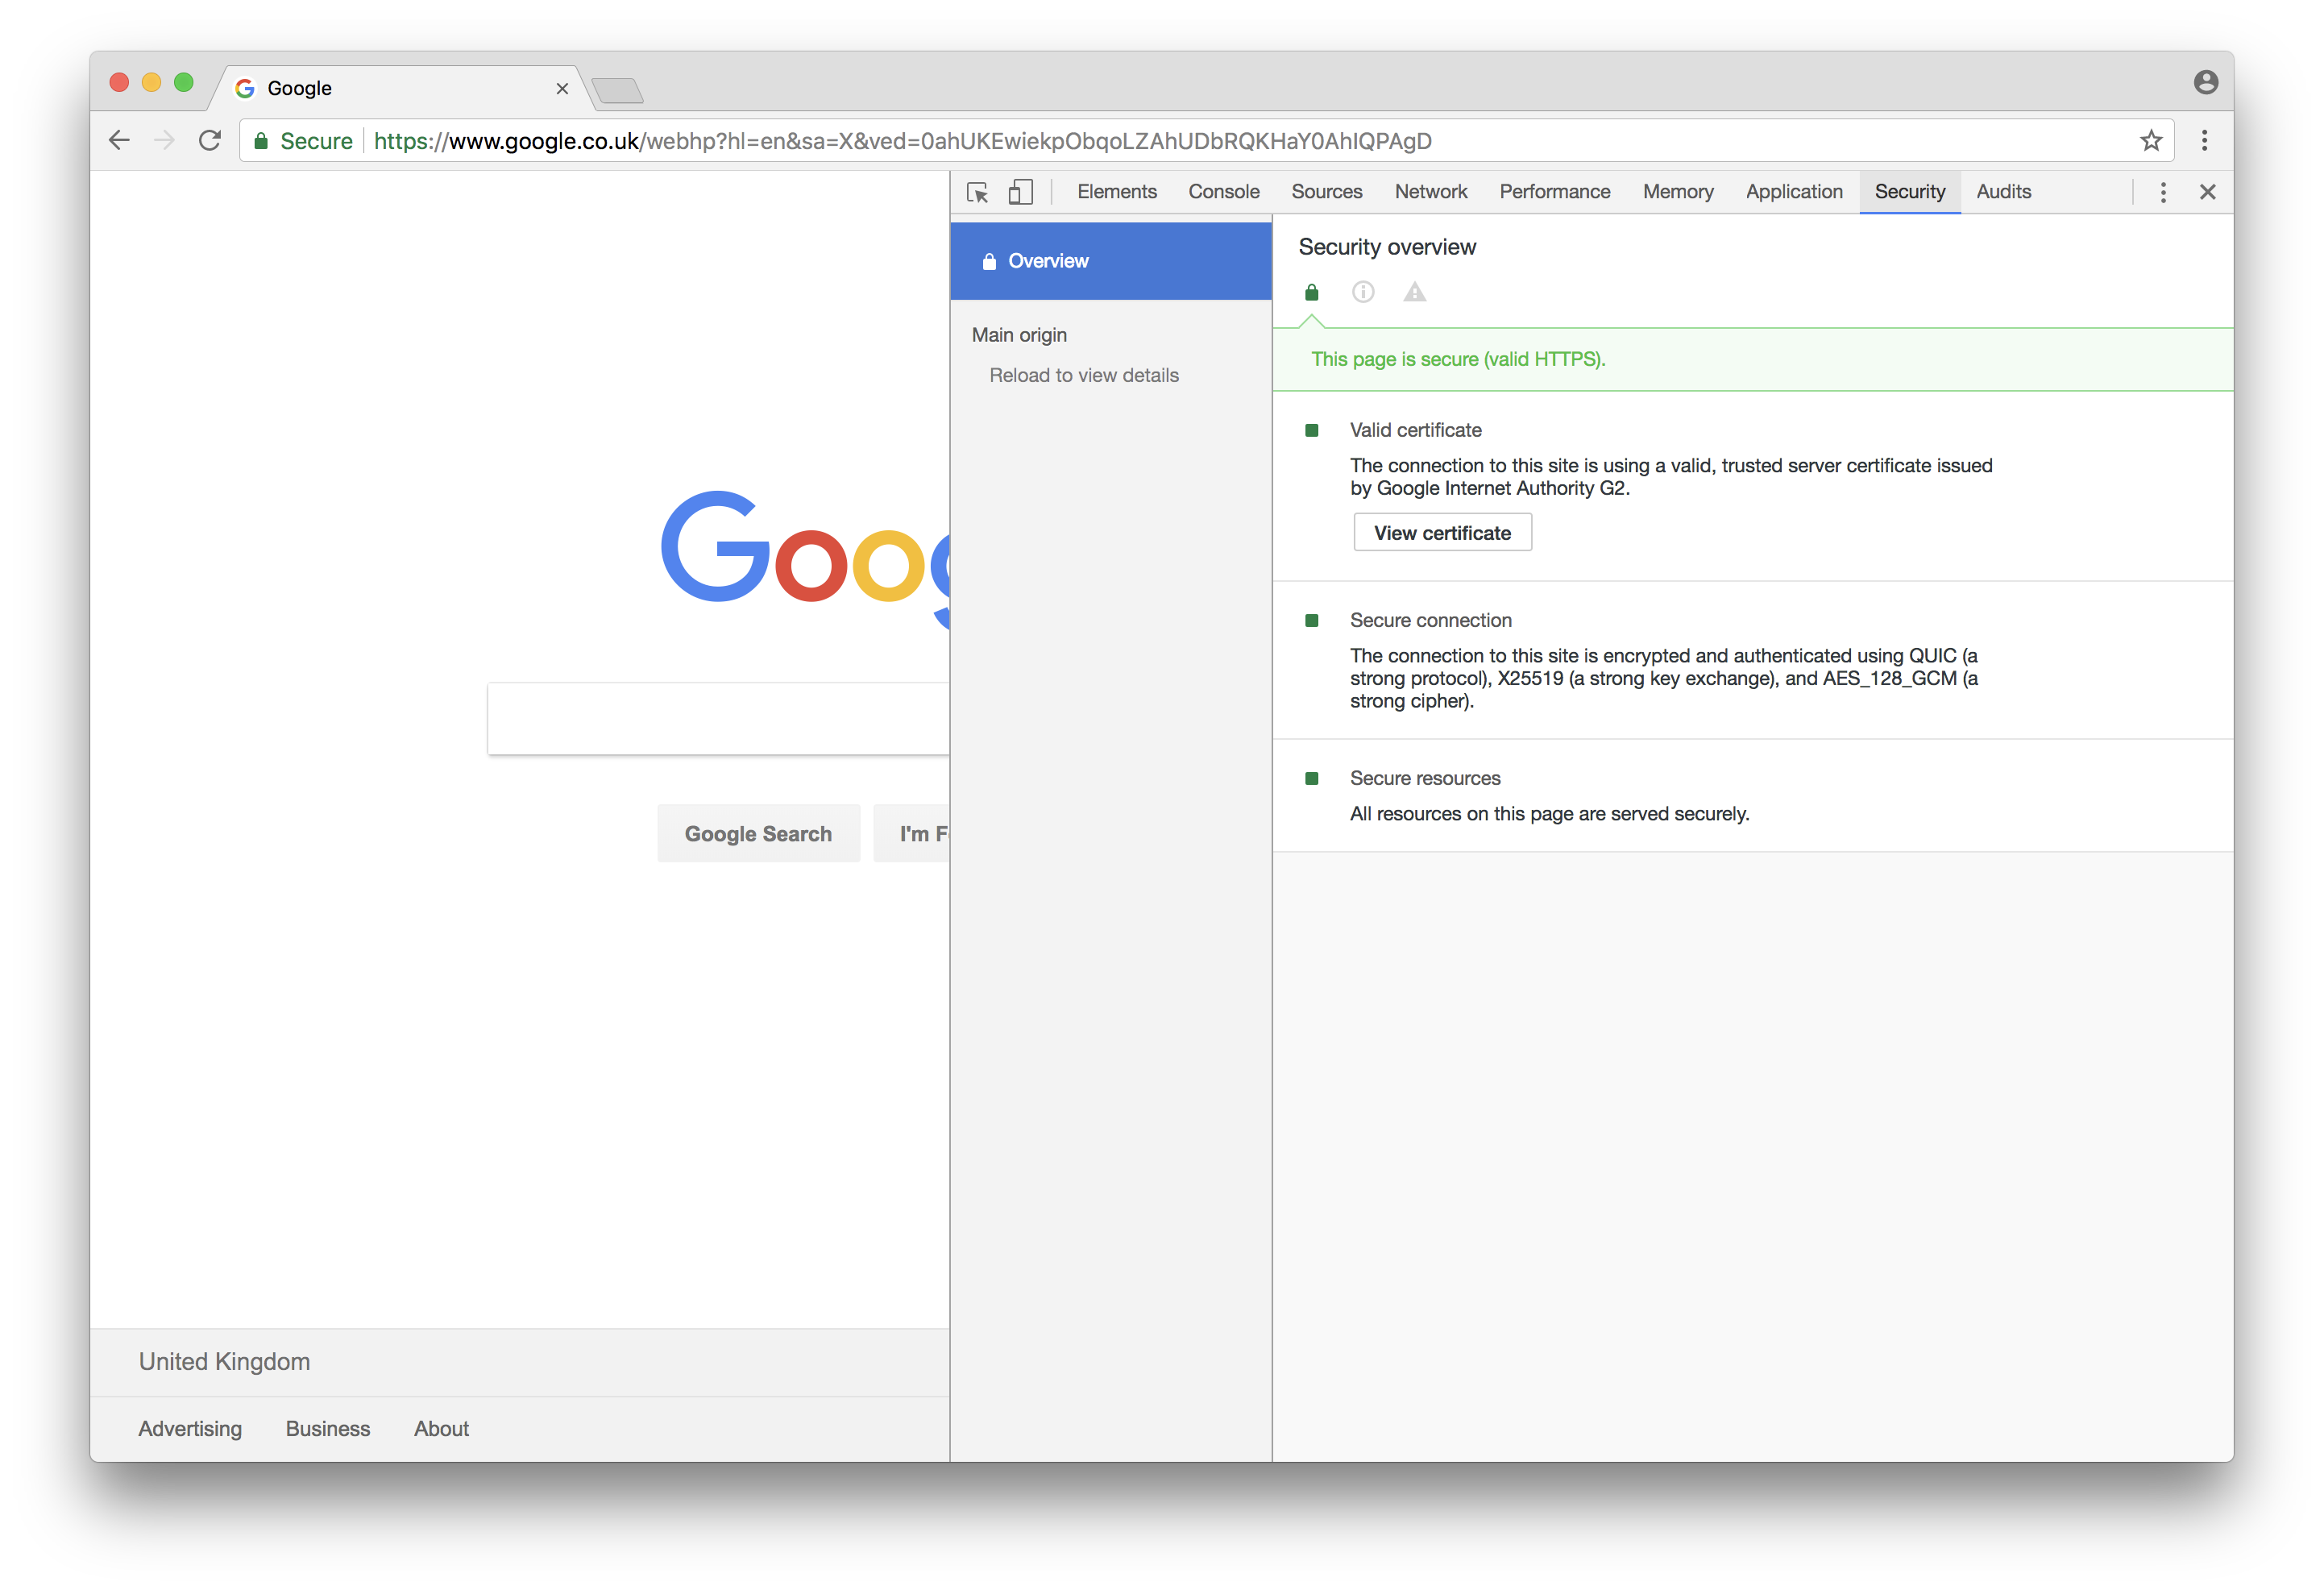
\includegraphics[width=0.8\textwidth]{figures/devtools-security.png}
\label{fig:devtools-security}
\end{figure}

\paragraph{} Finally, but no less important, Chrome supports an auditing feature using the Lighthouse project. This is a really useful tool for improving the quality of your pages. It audits against metrics for performance, accessibility, progressive web apps, search engine optimisation amongst many other aspects.

\begin{figure}[H]
\centering
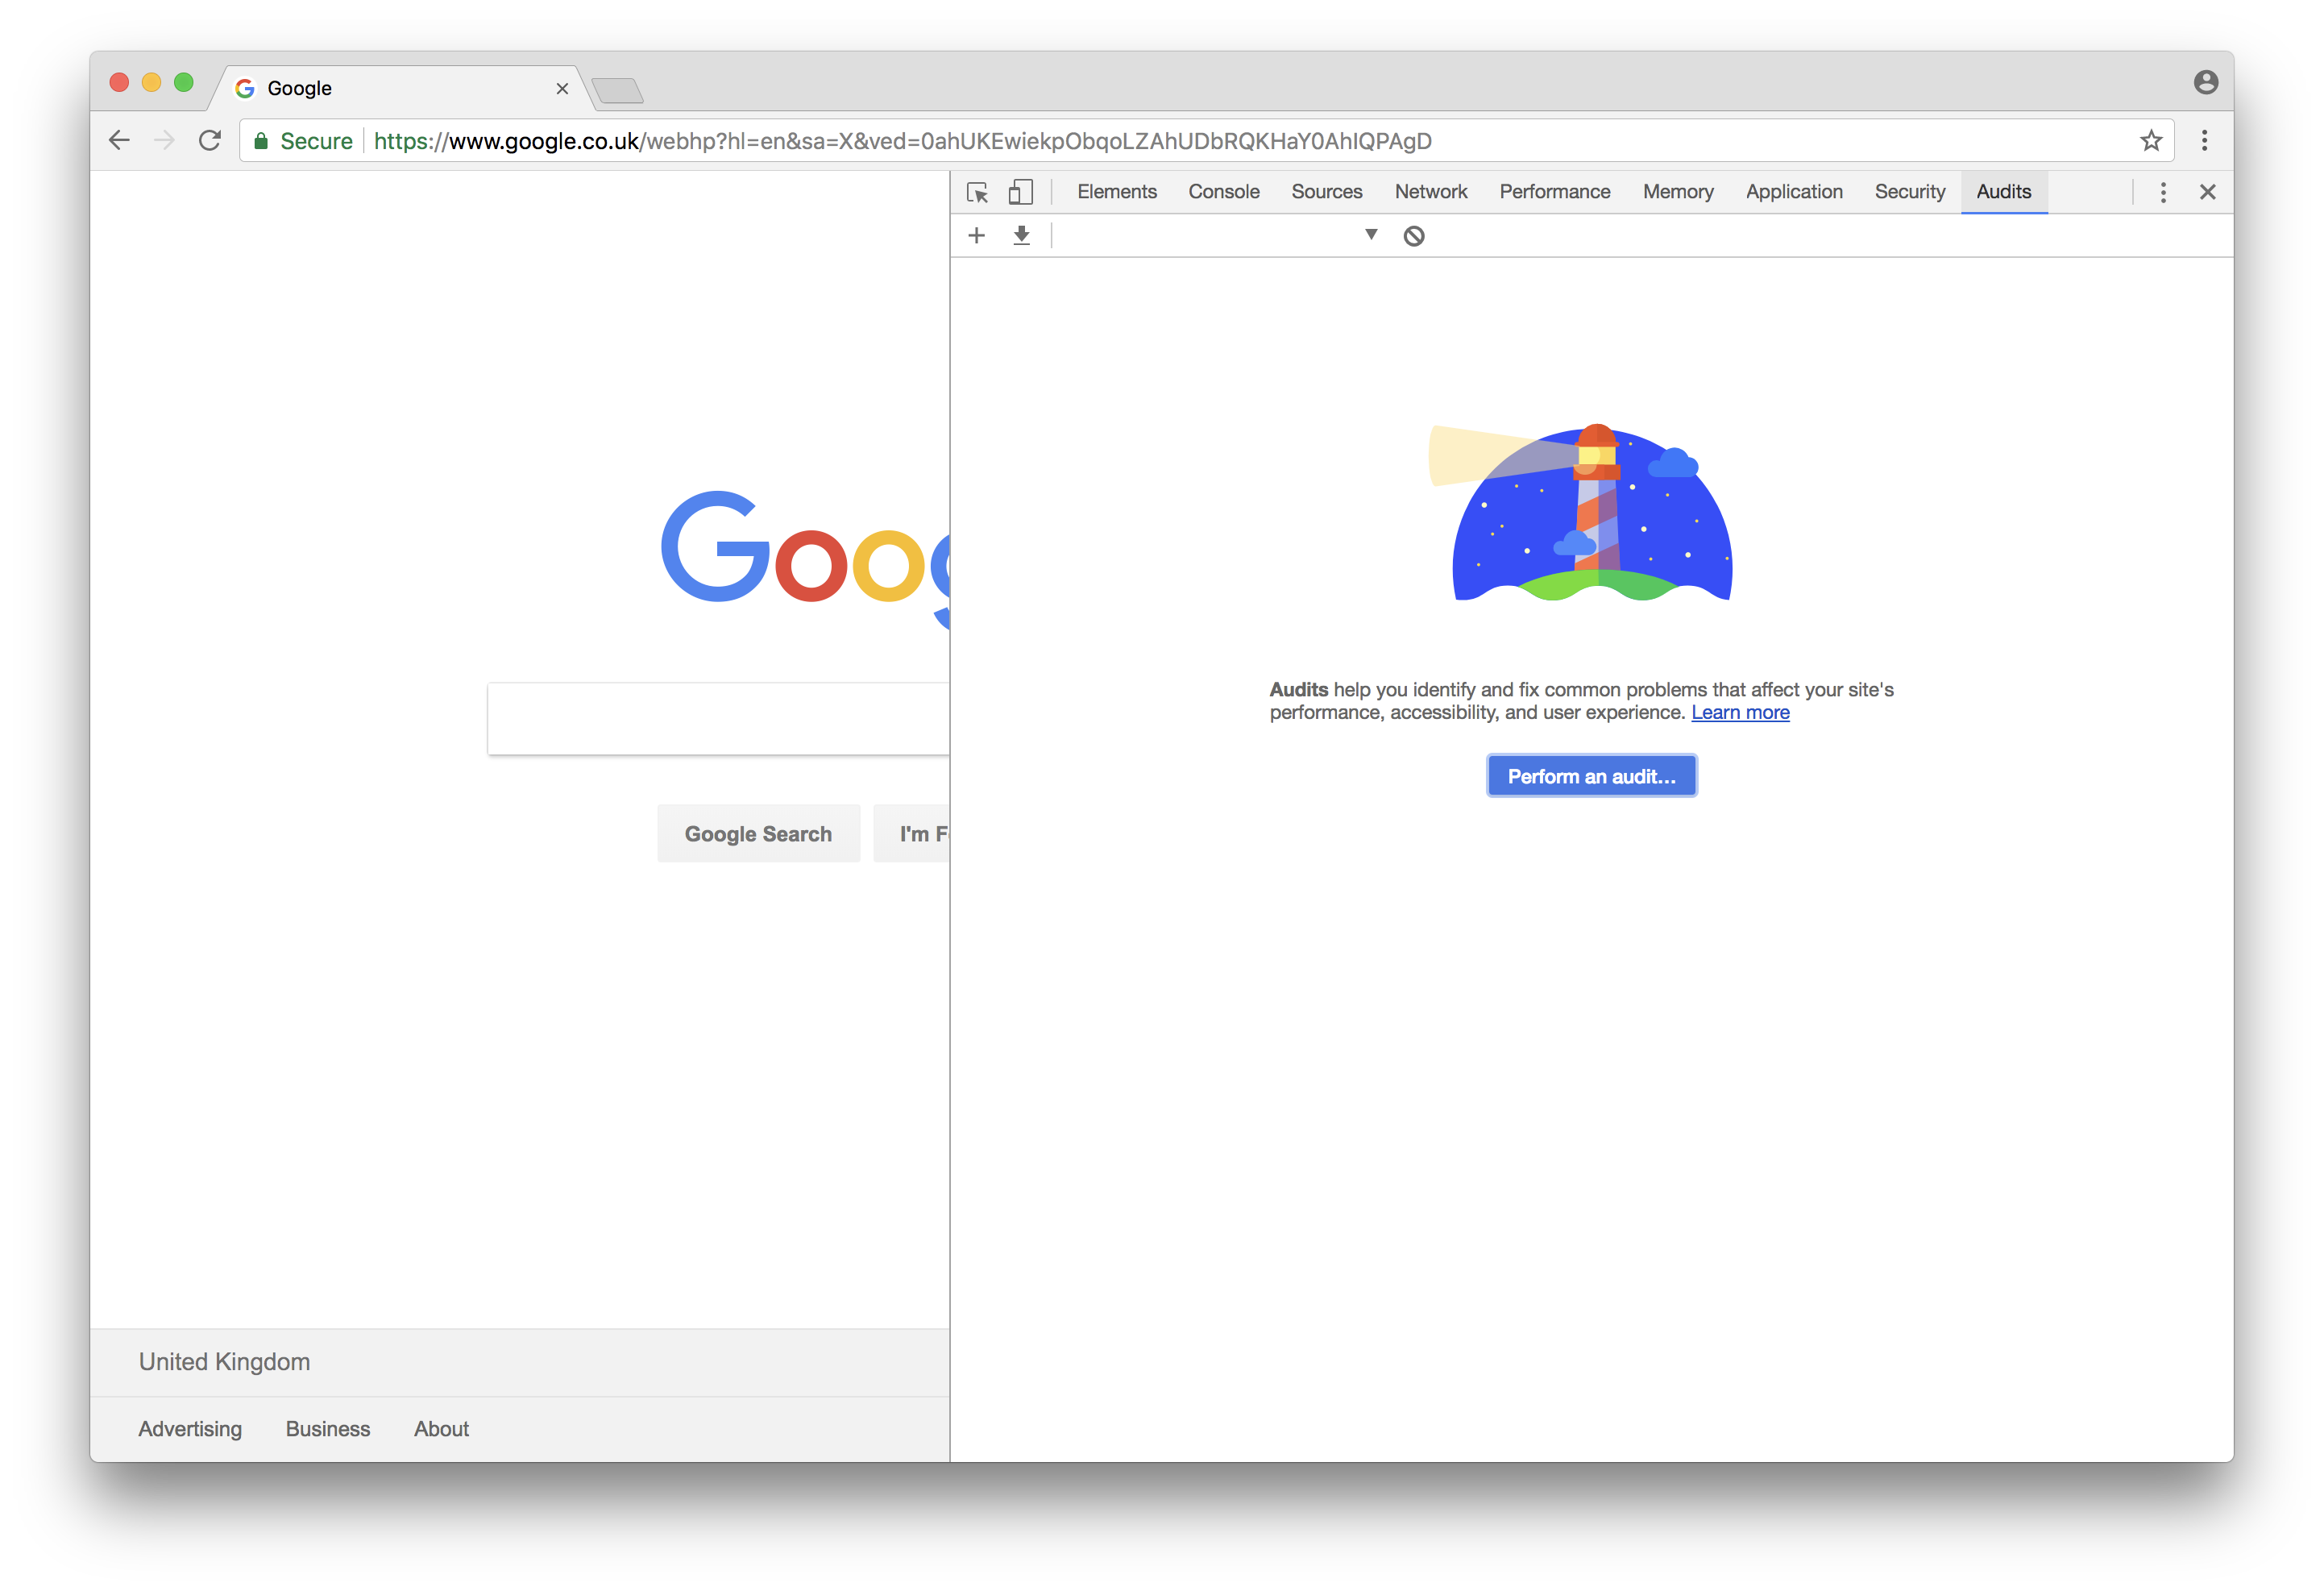
\includegraphics[width=0.8\textwidth]{figures/devtools-audits.png}
\label{fig:devtools-audits}
\end{figure}

\paragraph{} Throughout the remainder of this module, the browser tools will provide you with extrememly important insights into what your browser is doing at any given time. As your sites start to become more complex, you'll increasingly rely upon these tools to help you to track down the sources of bugs.


\section{Summary}
\paragraph{} Basically, before we can go anywhere, we should really know how we got to our current location. In this unit we've surveyed the following:

\begin{itemize}
\item A potted history of the Internet, Web, Hypertext, DOM, and Basic Web Architecture (Servers and Clients)
\item What happened technologically and socially, that lead to the situation we are in now
\item Overview of the basic things we need to know to understand how it all fits together
\end{itemize}

\paragraph{} We've also looked at the Chrome Browser features that we can exploit as a "development and learning environment" for this module.
\paragraph{} It may well be the case that you already knew about clients and servers, or HTML, CSS, and JS, or any of the other things that we've introduced in this unit. However, you should remember that this is only scratching the surface and is meant to bring us all to the same starting line, ready for the rest of the module. In all honesty, the complexity of the Web and its associated technologies, and the rapidity with which they are developing, means that there is far more to discover than it is possible for most people to know. Hopefully you've at least been introduced to some things that you hadn't thought about before. But if you are aware of all of this, then that is your cue to delve even deeper and to develop a thorough professional understanding.
\paragraph{} In summary, having read through all of the materials so far, and completed the practical work you should now have some idea of just how many different technologies interact to give us the Web that we know and love. You should also have some idea of the reasons why the Web that we have is the way that it is because of the incremental historical development of Web technologies over time, responding to user need. Finally, you should now have the minimal development environment that we'll need to progress through the rest of the units. Most important are the Chrome Browser, so that we have a default learning environment for everyone involved in the Module (which importantly incorporates useful debugging and development tools), an editor that can save plain text files (with .html, .css, and .js endings) so that we can write the source files that will make up our web pages as we progress.


\chapter{Hypertext + Markup + Information + Semantics = HTML}
\label{html}
\paragraph{} 


\chapter{CSS Intro \& Overview}
\label{css}
\paragraph{} 


\chapter{HTML Page Layout Using CSS}
\label{layout}
\paragraph{} HTML alone is really great, but pretty ugly. CSS gives us a way to improve how our pages are presented. We can use CSS and semantic HTML to group and organise elements of the UI to give us reusable ``blocks'' or `units'' from which any given page is assembled.
\paragraph{} The last chapter only scratched the surface of CSS and its interaction with, and applications to, Web design. We'll continue our study of CSS, but this time with a focus on the specific ways that CSS supports ``laying out'' or arranging the elements of a web page to achieve a particular design. You should contrast this with the last unit where we considered how individual typographical elements could be styled, such as the size or colour of lines of text. 
\paragraph{} Now, instead, we're thinking a little bigger, how all of the elements of a page work together to implement a design. Part of this story will be continued in the next unit when we consider some rules of thumb for designing pleasing user experiences. 
\paragraph{} For now though we'll consider how any given page can often be considered in terms of a number of blocks. Each block will gather together a number of html elements, for example, the header block, the footer block, the main content or "body" block, and the navigational block. When we start to think of our pages in terms of reusable blocks it can assist us both in designing our pages but also in terms of  implementing them as well.
\paragraph{} We've seen how HTML gives us essential structure for turning plain text documents into hypertext documents. To some degree HTML also gives us many of the structural elements that we are already used to in terms of word processing text documents. When we decide to make a line into a heading or add a break in our text to create a paragraph, these are similar processes whether we are using a word processor or writing HTML. However, these choices are concerned with capturing, or delineating, the different ways in which the parts of the document work together. Just marking something as a heading or a paragraph doesn't necessarily mean that it must be presented in any specific way. Instead it marks it out so that we can, if so desired, present it in a different way. This marking up process merely facilitates our being able to achieve this.
\paragraph{} To actually make a difference to how our HTML document, and the elements that make up that document, are actually seen by a user, we need to consider presentation. We use CSS to govern the visual presentation of our document, using the various elements of our HTML markup as cues to help us achieve this. 
\paragraph{} However, whilst CSS is concerned with visual presentation, this is not just making things look pretty. In addition, visual presentation via CSS is an important aspect of both usability and accessibility. By usability we mean all aspects of the design that make the resulting rendered page fit to address the task for which it was intended. Usability can range over many factors including safety, effectiveness, and efficiency. Accessibility is a related topic to usability which is concerned more with ensuring that the resulting design doesn't exclude users from effectively using it. This could include ensuring that a page is accessible to people with specific disabilities, for example, making a page accessible to those with visual impairment might require the underlying HTML to be effectively structured for an assistive technology such as a screen reader to use it. However not all visual impairments are equal, another view on the same aspect of accessibility might require that colour contrast be sufficient between background and foreground elements so that those with minor visual impairments can effectively use the site, whereas colour selection, the choice of colours for a site's colour scheme shouldn't exclude those, or reduce accessibility for those with colour vision deficiency or colour blindness. To root this in the real world consider that red-green colour blindness affects up to 8\% of males of Northern European descent.
\paragraph{} In the last unit we dealt with styling individual elements but now let's consider how we can group HTML elements together so that they can be managed, laid out, and presented to our users regardless of the device they use. By doing this kind of approach, we also start to gain some strategies for managing a site's design, rather than merely the design of a single page. By reusing groups of elements in similar ways across different pages, we can begin to produce designs that have consistency, and which, as a result, provide a better user experience.
\paragraph{} Before we get deeper into this unit, let's also consider just how good the browser is at rendering web pages. Whilst CSS is useful for styling HTML and can make things look great, allowing the browser (user agent) to decide how to place HTML elements on screen is frequently a great idea. The main reason is that this is what the browser, or more correctly, the browser's page layout engine, is designed to do. You can however override this behaviour to get your pages to be laid out and rendered in other ways. CSS will influence how things look and where they are placed. You should recognise though that the more you override the browsers default approach to page layout, the more work you are making for yourself and the more likely you are to run into cross-browser inconsistencies that can lead to different behaviour on different platforms.


\section{Rendering Pages}
\paragraph{} Our browser is designed to render web pages. That is, it retrieves the HTML for the page associated with the current web address, then retrieves any linked resources including CSS and JS as well as things like images. During this process the browser will parse the HTML and create an internal DOM representation of the page, modifying this as necessary to account for any directives from the CSS or any modifications imposed by the JS. 
\paragraph{} Unless the CSS or JS overrides the default layout that the browser uses then most pages are laid out fairly simply. Assuming a left-to-right reading order, rendering begins at the top left corner and the page flows from there in the order in which it is defined in the HTML document. This is generally a straightforward process which, as a rule, is only hindered by images of unknown dimensions which take longer to download than the rendering engine takes to layout the page according to the known information. This is one reason why you might occasionally see pages that seem to change where things are located as images appear, because the dimensions weren't specified in the HTML and could only be finalised once the associated image file was fully retrieved.
\paragraph{} Sometimes though, we really want to have more control over our layout. We want to be able to create a block, or grouping of items, that are placed in a specific location on screen, e.g. to the left, or right, or above, or below other items. Essentially we want to place our HTML elements in particular locations on screen where the normal layout engine, uninterrupted, wouldn't normally put them. This creates tension because browsers are built around layout engines which are optimised for presenting documents, particularly documents that have a quasi-academic publication style structure including, for example, an introduction, various sub-sections, and a conclusion.
\paragraph{} Any other form of screen layout, such as a desktop application style user interface, will potentially cause issues for the layout engine. For example, requiring multiple passes to place things in their correct position, or even not being able to consistently and comprehensively satisfy all of the constraints that the design imposes. Remember also that the rendering engine is trying to, by default, create the best layout for the current combination of screen quality and window dimensions, given the content that has to be displayed, and, for the most part, the current generation of rendering engines do a really good job when designers respect this.
\paragraph{} We should note that text is inherently responsive by default. It can keep wrapping to the next line until you reach the end of the content. Text resizes nicely to account for all devices, screens, viewports, and window sizes, resolutions, pixel densities, and dimensions. It just keeps flowing until the page is done. 
However when we try to use the same rendering engine for more exacting layouts, trying to implement desktop style interfaces for example, difficulties can, and frequently do, arise.



\section{Layouts: HTML + CSS}
\paragraph{} Let's now look at a way to do layouts with CSS and HTML versions earlier that HTML5 that you will see in the wild, and which work, but that are no longer the preferred approaches. Note that this is for historical usage only; we'll look at some better ways to implement modern designs using HTML5 and CSS, but currently you also need to be aware of the approaches that are still out there. Because many sites have used these approaches, they will be around for a long time, and you might be called upon to maintain such a site in your career.
\paragraph{} You can use HTML <span> and <div> elements to assemble page layouts. These elements work in different ways and introduce two useful notions to our design toolset. The first is the idea of an inline element, something that works within the context of, or inline with, another element. For example, given a paragraph of text, if you want to have a specific sub-string treated in a different way, such as coloured for emphasis, then an inline element is useful to mark up the start and end of the sub string. The span element is just such an inline element and that's exactly how we might use it. Contrast that with the div element which enables us to wrap parts of our page into a block, to group elements, so that we can treat the contents of the block differently from the rest of the page.
\paragraph{} If we wrap these inline and block elements around the different groups of content of our page we can then target those groups with specific CSS. This is achieved by given each inline and block element a unique ID attribute so that they can be identified, referenced, and subsequently positioned and styled by CSS. Note that to do this, HTML requires IDs to be unique.
\paragraph{} You'll see this pattern in lots of web sites built prior to HTML5. For quite a while this was an effective way to control the layout of a page but it had, and still has, drawbacks. The main drawback is that your choice of ID for each grouping might not have the same semantic communicative ability as the IDs that others are using. Also the sheer variety of ways in which we can say the same thing, e.g. referring to the navigation bar which we could call ``navigation bar'' or just ``navigation'' or ``navbar'' or ``nav-bar'' or merely ``nav''. If it is a panel down the side then we can add all the combinations of nav and panel to the list above. Instead it is best to use semantic HTML tags to achieve this kind of layout control when possible. 
\paragraph{} But what if you have groupings that don’t fit to standard semantic tags? For example, for columns of content in a multi-column layout for ultra-wide monitors. At this point, the use of div blocks makes sense again, as a way to take us beyond the language that HTML 5 semantics define, but not as a starting place.


\section{How Not To Lay Out Pages}
\paragraph{} Using div and span tags to organise a page layout isn't the only way that web developers have tried to produce pixel perfect layouts and desktop style user interfaces in the past. So let's quickly survey some of the approaches for how not to do it.
\paragraph{} One method was to misuse HTML tables. Because tables arrange things semantically into columns and rows, it is an easy mis-step to get from there to the idea that this semantic use can extend to the visual presentational use. However tables are, just like most default HTML elements, inherently responsive, they will reflow to best fit the screen and window that they are rendering for. This means that changing the window dimensions can alter the layout of the page contents as the text reflows. A clever hack involved combining a table with single pixel transparent gif image files. As they are transparent, the user doesn't see the files, but by using many of them they can be used to push page content around so that it is laid out just as the designer intended for it to be seen visually. However, this is a horrible solution to the problem of getting HTML layout engines to do something they weren’t designed to. The main problem being that this is not easily maintainable and can have lots of side-effects for accessibility because a page might now incorporate many thousands of instances of transparent gifs. Think about it, to indent a line of text by 300 pixels will need 300 single pixel gifs.
\paragraph{} In comparison to this, the use of divs and spans to group elements then CSS to arrange them is much better; whilst this is still horrible and severely breaks semantic HTML the impact is less terrible but far from ideal.



\section{Some Common Layouts}
\paragraph{} Before we get to actually using CSS to lay out our pages, let's just consider some basic layouts that are quite common.
\paragraph{} The default for the web is as a single column of text which reflows according to the dimensions of the window that it is rendered to. This is inherently reliable, stable, and responsive. However, as the size of page content increases, this can become a little unwieldy, not necessarily unusable, but, for example, the amount of scrolling required to reach the top or bottom of the page can increase significantly. Similarly, such a page might require the user to find the exact hyperlink, embedded in the page, to enable them to navigate to other pages in the site.
\paragraph{} This leads to the category of layouts that involve two parts, the content part, and the navigational part. By grouping all of the links to other pages in the site together, a consistent navigation experience can be designed and replicated relatively easily across all pages in the site so that your users know where to look to find the next place to navigate to. This is generally laid out in one of four ways, with navigation above, or below, or to the left of, or to the right of, the page content. Frequently this leads to a two column layout, with a navigation bar to the left, or right, and the content next to it. This might also include CSS directives to stop the navigation element from scrolling when the rest of the content is bigger than the screen.
\paragraph{} Yet another, reasonably common layout, again with multiple possible variations is the three column layout, including a navigation bar and content, but now with the addition of some kind of sidebar which perhaps incorporates additional data or metadata about the current page.
\paragraph{} You are only really limited by practicality in terms of potential layouts involving some combinations of multiple rows or columns. Note however that a common extension of these layouts is also to include a header and, or, footer area at the top and, or, bottom of the screen respectively. These might well also combine with the navigational aspects, depending upon your design goals for the page.
\paragraph{} Additionally, consider that many sites will also incorporate some dynamic elements in their page layout, for example, enabling hide-able panels or modals that can be shown or hidden as necessary.



\section{CSS-based Layout Solutions}
\paragraph{} Two recent solutions give better control over relative placement of HTML elements than using divs and spans and can enable us to realise some of the layouts we've considered whilst maintaining much of the basic flexibility and responsiveness of traditional HTML. These include the FlexBox and the Grid layout. Each is potentially applied to multiple collections of elements to place them relative to each other on screen during rendering.
\paragraph{} The Flexbox is a way to lay out linear collections of elements either horizontally or vertically. That basically means placing collections next to each other, from the left edge of the screen until the right edge is met, then wrapping around to put the next collection below the others and continuing to place collections in this manner, wrapping around as needed, until everything is laid out. If we consider each collection to be a word in a sentence, which is really a collection of letters, then this is just like how a sentence is placed on a page, running from left margin to right, and wrapping around into another line each time it reaches the right margin.
\paragraph{} The Grid Layout is similar, but instead of working in a single, linear dimension, it works in two dimensions, and is a way to lay out matrices of elements as rows and columns. In some ways this is just a like a table, but recall that an HTML table is for organising matrices of information semantically, a Grid layout is for presenting matrices of information visually. This means that if we want to enforce that a certain group of information is always vertically aligned above or below another group, or immediately to the left or right of another group, we now have a mechanism to do so.
\paragraph{} Both the Flexbox and Grid are designed to use CSS to influence the visual placement of HTML elements so that we can avoid hacks like using the transparent gif when attempting to implement our desired layouts.
\paragraph{} When considering the use of FlexBox and Grid layout we should take into account the following:

\begin{itemize}
\item How we build interfaces — there are certain recurrent patterns of user interface layout as we considered earlier.
\item How pages are rendered — from the upper left corner of the screen to the lower right corner of the screen.
\item That the screen has two dimensions — the horizontal dimension and the vertical dimension.
\end{itemize}

\paragraph{} So, in some cases we want to lay out things in one single dimension, either horizontally or vertically, but not both at the same time. This leads naturally to the idea of the FlexBox. A layout for a collection of items along a single dimension. Where the FlexBox works either horizontally or vertically, if we add the second, complementary, dimension, then we arrive at the Grid layout.
\paragraph{} Let's now consider each approach in turn, starting with the FlexBox\dots



\section{FlexBox}
\paragraph{} Imagine a box reaching horizontally from one side of the screen to the other. This box can contain HTML elements, either as individuals, or in groups. We want to be able to control how elements are spread across the box from one side of the screen to the other. For example, we might want to control the amount of space to either side of, and between, the elements in the box.
\paragraph{} Because our computer screens are not infinitely wide or high, we can't have our box containing infinite elements. At some point, if we have sufficient content, we reach the edge of the screen, and the responsive nature of our browsers rendering engine will attempt to reflow the content to start on the next "line" below. If our screen is too narrow for the content we want to display then we might also want to be able to exercise a little control over how and when the box flows over into another row and arranges elements below.
\paragraph{} Note that there are some minor differences between horizontal and vertical arrangements because we are habitually used to scrolling up and down a page, but less used to scrolling horizontally, so reflowing content that is too wide for the screen so that it is displayed below seems sensible, but for vertical arrangements, we expect to just keep scrolling down until we reach the end.
\paragraph{} Flexbox lets us do this. It supports a range of CSS properties:

\begin{itemize}
\item flex
\item flex-basis
\item flex-direction
\item flex-flow
\item flex-grow
\item flex-shrink
\item flex-wrap
\end{itemize}

\paragraph{} For each property you should investigate the documentation associated with it in the Mozilla developer Network CSS reference\footnote{\url{https://developer.mozilla.org/en-US/docs/Web/CSS/Reference}}. Let's now consider some examples to see what FlexBox looks like and how it can be used.




\section{Flexbox Resizing Example}
\paragraph{} This example is meant to demonstrate a very simple collection of content and how FlexBox can manage the arrangement of that content when a window's dimensions are altered. We'll use FlexBox to style an unordered HTML list.
\paragraph{} First, some HTML (flex1.html) for our page. It's worth taking a look at how this is rendered without the CSS so that you get an idea of what it looks like in isolation without any CSS applied. This will let you see just how much functionality the CSS Flexbox declaration adds.

\begin{lstlisting}
<!DOCTYPE html>
<html lang="en">
	<head>
		<meta charset="UTF-8">
  		<title>CSS Flexbox</title>
  		<link rel="stylesheet" href="flex1.css">
	</head>
	<body>
		<ul class="flex-container">
			<li class="flex-item">1</li>
			<li class="flex-item">2</li>
			<li class="flex-item">3</li>
			<li class="flex-item">4</li>
			<li class="flex-item">5</li>
			<li class="flex-item">6</li>
		</ul>
	</body>
</html>
\end{lstlisting}

\paragraph{} Note that we just have a simple HTML document, with a link to an external CSS file. In the body of our document we merely have an unordered list whose contents are the numbers 1 through 6. This is merely to make it easy to see and compare how the contents of the FlexBox are placed and rendered. See that the <ul> tag has a flex-container class attribute and the individual items are given flex-item class attributes. Now let's get to the CSS (flex1.css).

\begin{lstlisting}

.flex-container {
  padding: 0;
  margin: 0;
  list-style: none;
  display: flex;
  flex-flow: row wrap;
  justify-content: space-around;
}

.flex-item {
  background: tomato;
  padding: 5px;
  width: 200px;
  height: 150px;
  margin-top: 10px;
  
  line-height: 150px;
  color: white;
  font-weight: bold;
  font-size: 3em;
  text-align: center;
}
\end{lstlisting}

\paragraph{} All we have done here is apply styling to the unordered list container, indicating that we want it treated as a flex container with the display:flex and flex:flow directives. We've also applied a style for individual items within the container. This is all standard CSS and not specific to the FlexBox container but merely changes colour and font settings, as well as adding padding and sizing information to the elements.
\paragraph{} This should give us a set of 6 boxes which will reorganise themselves to best use the space available in the enclosing window. Here is what it should look like but you should really try it out for yourself and experiment with things to get a feel for how the FlexBox acts.


\begin{figure}[H]
\centering
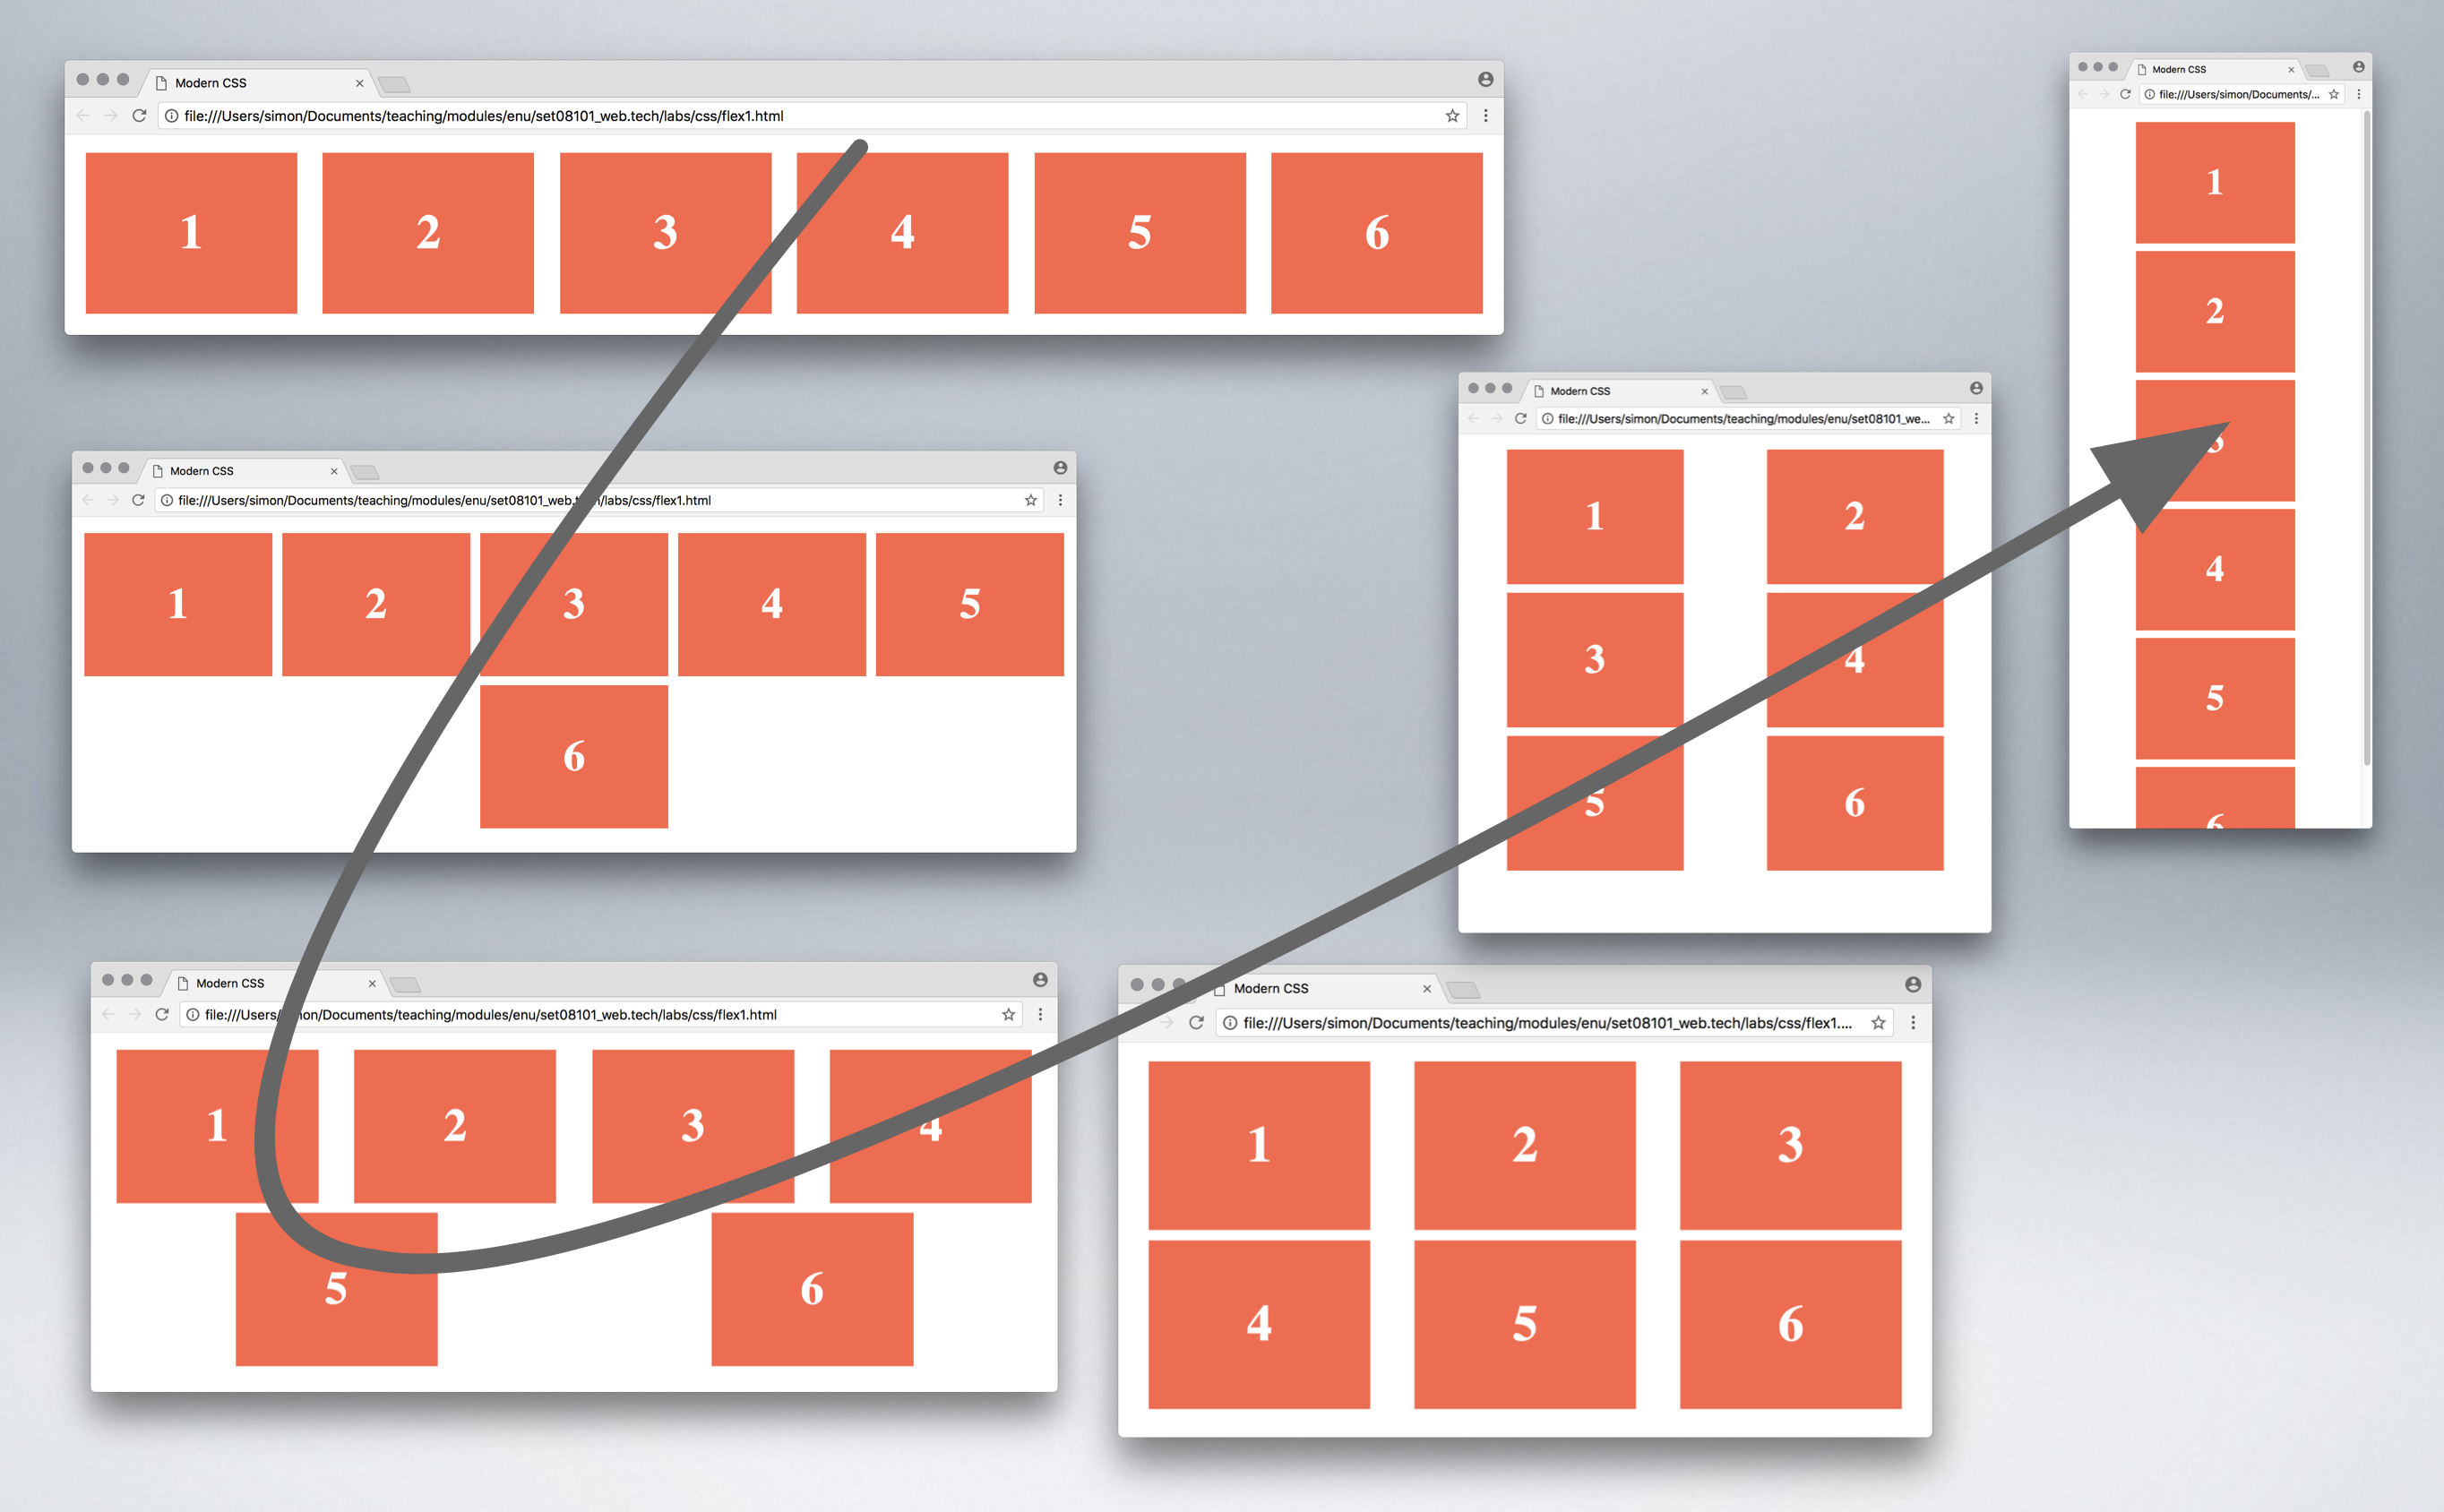
\includegraphics[width=0.8\textwidth]{figures/flexbox-resizing-example}
\label{fig:flexbox-resizing-example}
\caption{}
\end{figure}




\section{Flexbox Navbar}
\paragraph{} One useful application of the FlexBox is to help implement a navigation bar, or navbar, which will reflow to make the best use of the enclosing window whilst remaining enclosed and isolated from surrounding HTML elements in the same document. This is a common layout design that is worth having in your toolbox.
\paragraph{} Let's see what a simple navbar would look like using the FlexBox. First some HTML (flex2.html):

\begin{lstlisting}
<!DOCTYPE html>
<html lang="en">
	<head>
		<meta charset="UTF-8">
  		<title>Flexbox Navbar</title>
  		<link rel="stylesheet" href="flex2.css">
	</head>
	<body>
		<ul class="navigation">
  			<li><a href="#">Home</a></li>
  			<li><a href="#">About</a></li>
  			<li><a href="#">Products</a></li>
  			<li><a href="#">Contact</a></li>
		</ul>
	</body>
</html>
\end{lstlisting}

\paragraph{} This is fairly straightforward HTML content. Like our last example, an unordered HTML list, but instead of merely numbers as content, we've named each item according to how it might be named for a simple online business, and turned each item into an empty hyperlink because the purpose of a navbar is to help us to navigate to different locations in the site. Now let's investigate the CSS (flex2.css) to style this as a FlexBox navbar. It's a bit more complicated than the simple demonstration earlier. If in doubt look up the CSS declarations that you are unfamiliar with in the MDN CSS reference.



\begin{lstlisting}
.navigation { 
    list-style: none; 
    margin: 0;
    background: tomato; 
    display: flex;
    flex-flow: row wrap;
    justify-content: flex-end;
}
.navigation a { 
    text-decoration: none; 
    display: block; 
    padding: 1em;
    color: white;
}
.navigation a:hover {
    background: darken(tomato , 2%);
}
@media all and (max-width: 800px) { 
    .navigation {
        justify-content: space-around; 
    }
}
@media all and (max-width: 600px) { 
    .navigation {
        flex-flow: column wrap;
        padding: 0; 
    }
    .navigation a {
        text-align: center;
        padding: 10px;
        border-top: 1px solid rgba(255,255,255,0.3); 
        border-bottom: 1px solid rgba(0,0,0,0.1);
    }
    .navigation li:last-of-type a { 
        border-bottom: none;
    } 
}
\end{lstlisting}

\paragraph{} Part of this complexity is just to manage things like the display of hyperlinks in the navbar. Now let's see how that looks:


\begin{figure}[H]
\centering
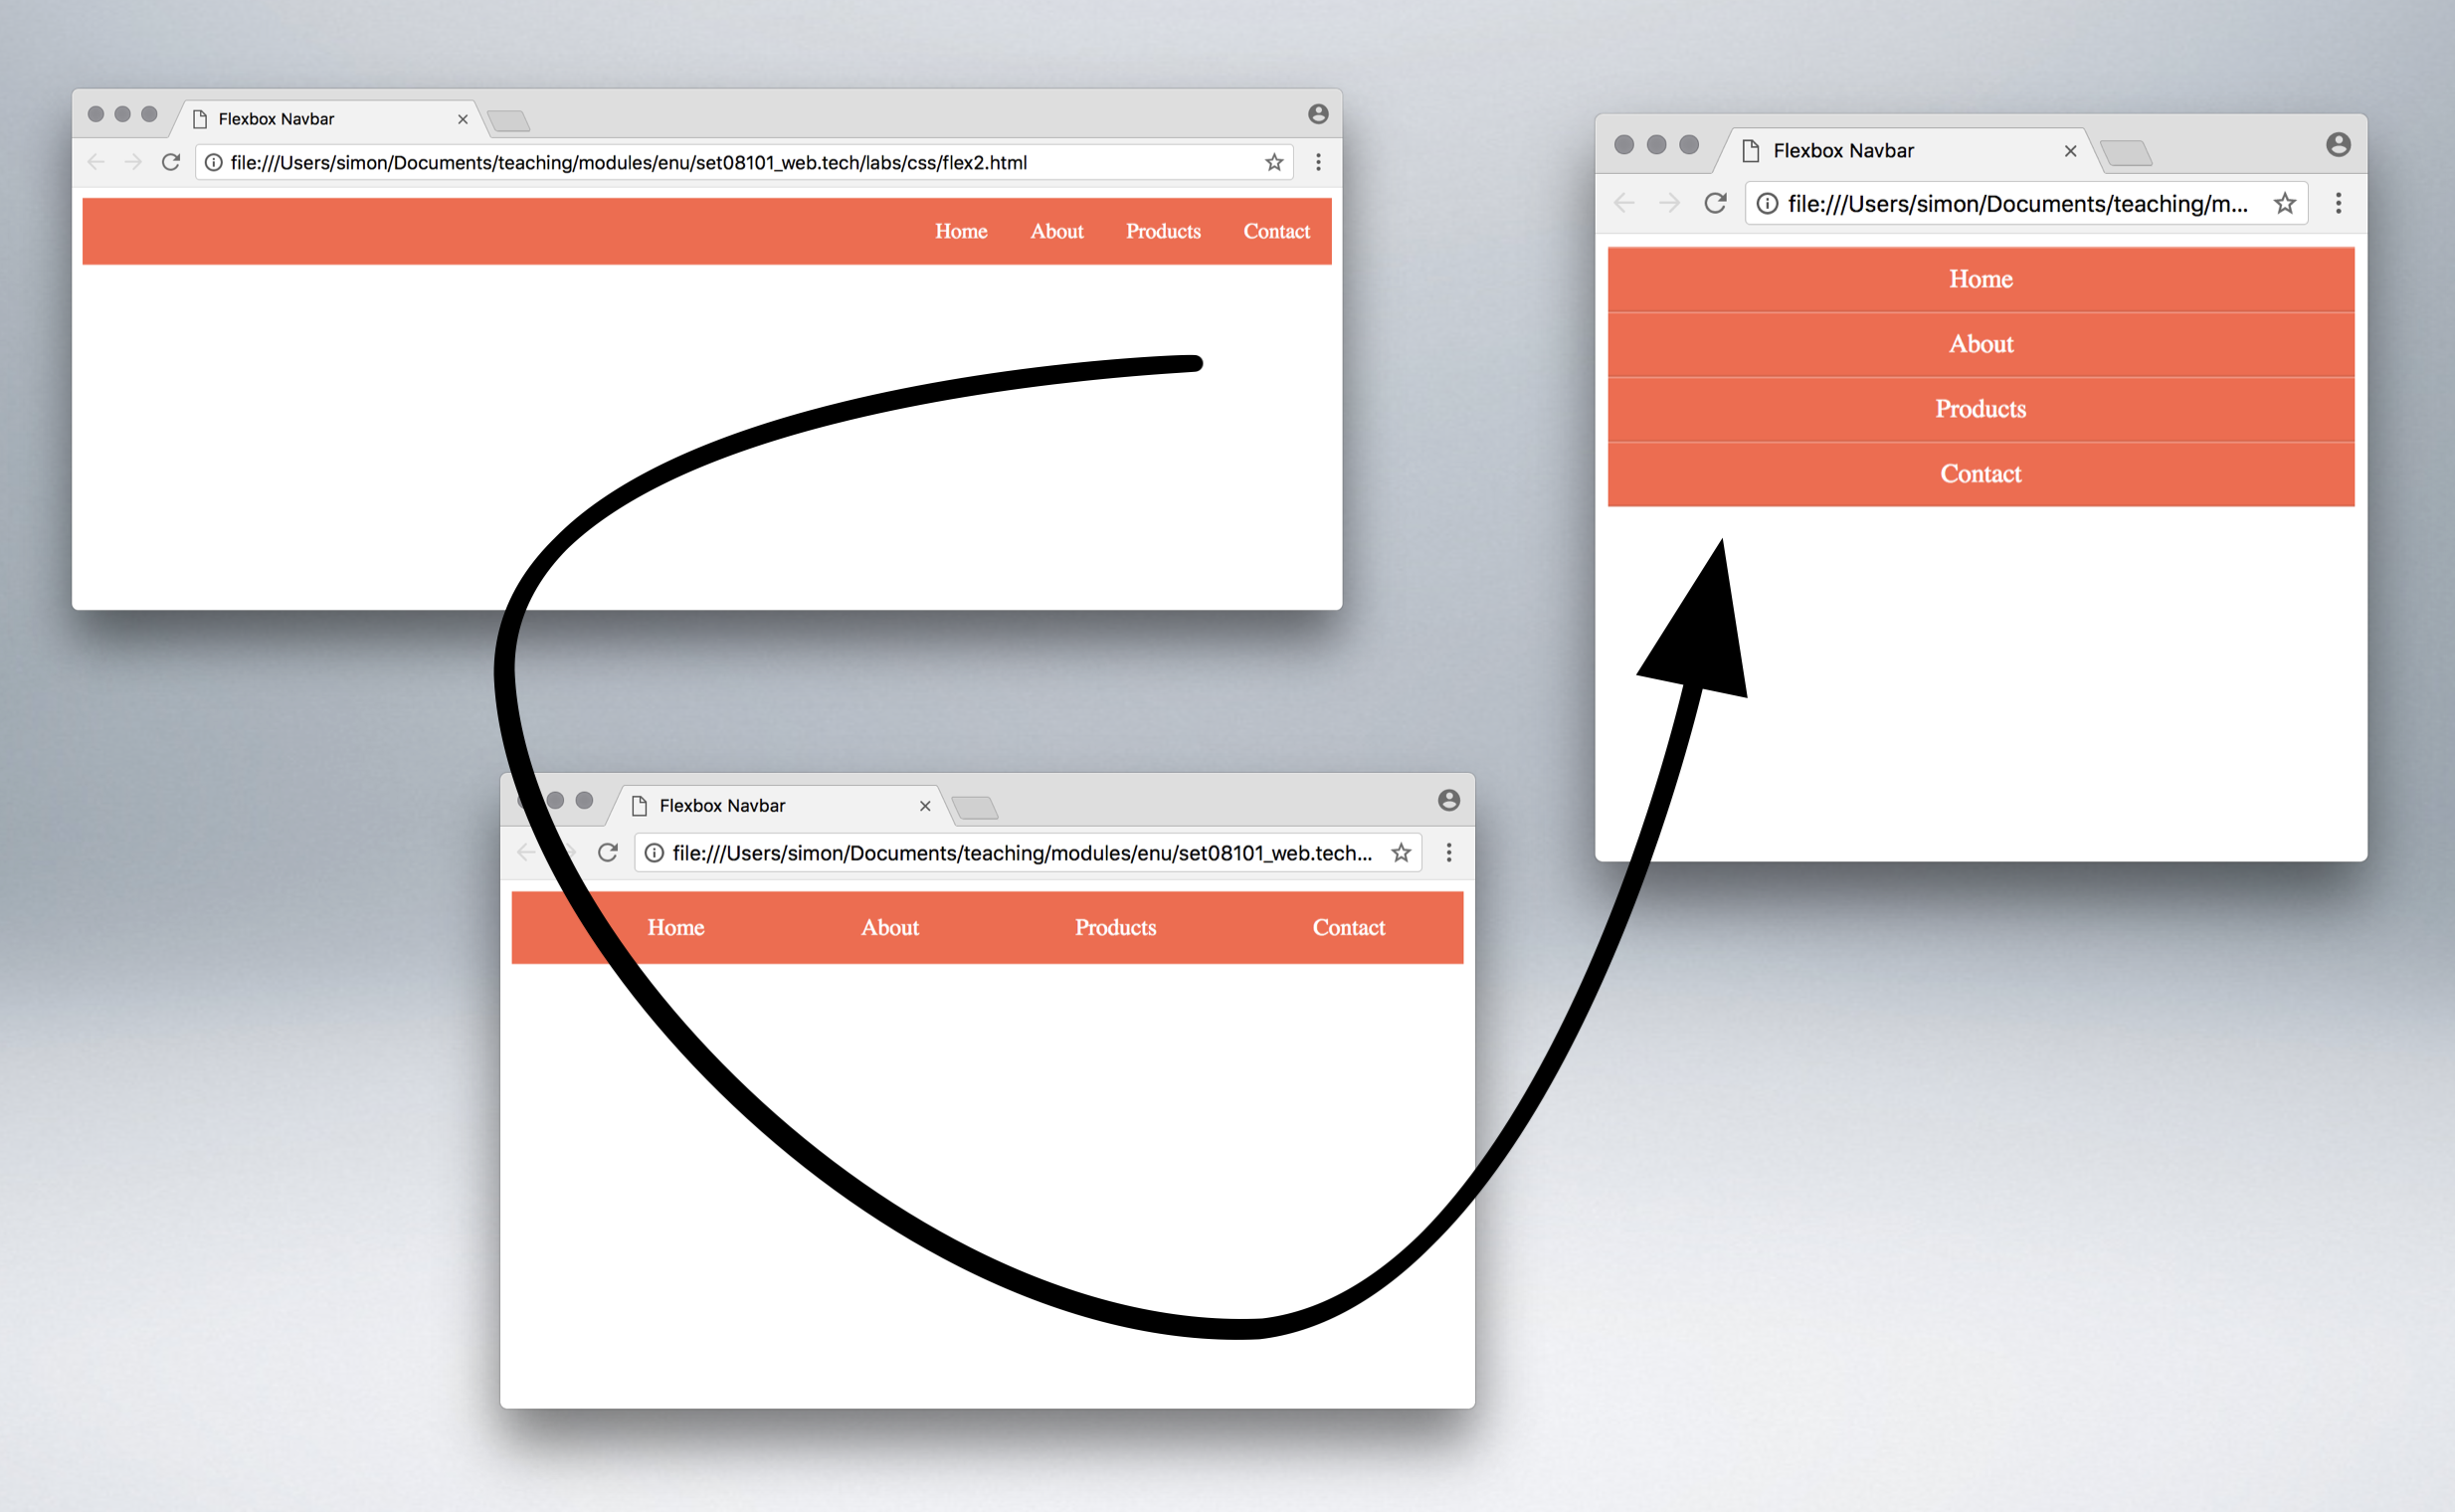
\includegraphics[width=0.8\textwidth]{figures/flexbox-navbar-example}
\label{fig:flexbox-navbar-example}
\caption{}
\end{figure}



\section{Flexbox Page Layouts}
\paragraph{} There's nothing to stop us going further than merely creating a flexible navigation bar. Instead we could use a flexbox to lay out our entire page. Let's give that a go. Note in the example how we are now using semantic HTML5 elements like the header, article, aside, and footer. Note that we're also wrapping everything in a div so that we can apply the display: flex declaration to all of the page's body content. First the HTML (flex3.html
):

\begin{lstlisting}
<!DOCTYPE html>
<html lang="en">
	<head>
		<meta charset="UTF-8">
  		<title>3-column layout + full-width header and footer</title>
  		<link rel="stylesheet" href="flex3.css">
	</head>
	<body>
		<div class="wrapper">
			<header class="header">Yar Pirate Ipsum</header>
  			<article class="main">
    				<p>Deadlights jack lad schooner scallywag dance the hempen jig carouser broadside cable strike colors. Bring a spring upon her cable holystone blow the man down spanker Shiver me timbers to go on account lookout wherry doubloon chase. Belay yo-ho-ho keelhaul squiffy black spot yardarm spyglass sheet transom heave to.</p>  
  			</article>
  			<aside class="aside aside-1">Aside 1</aside>
  			<aside class="aside aside-2">Aside 2</aside>
  			<footer class="footer">Footer</footer>
		</div>
	</body>
</html>
\end{lstlisting}

\paragraph{} Note that we're using some ``placeholder text'' to fill out the various parts of the interface so that the layout engine in the browser actually has something to lay out. Now let's take a look at the CSS (flex3.css):

\begin{lstlisting}
.wrapper {
  display: flex;  
  flex-flow: row wrap;
  font-weight: bold;
  text-align: center;
}

.wrapper > * {
  padding: 10px;
  flex: 1 100%;
}

.header {
  background: #CC3F0C;
}

.footer {
  background: #9A6D38;
}

.main {
  text-align: left;
  background: #33673B;
}

.aside-1 {
  background: #D8CBC7;
}

.aside-2 {
  background: #D8CBC7;
}

@media all and (min-width: 600px) {
  .aside { flex: 1 0 0; }
}

@media all and (min-width: 800px) {
  .main    { flex: 4 0px; }
  .aside-1 { order: 2; } 
  .main    { order: 3; }
  .aside-2 { order: 4; }
  .footer  { order: 5; }
  .header   {order: 1;}
}

body {
  padding: 2em; 
}
\end{lstlisting}

\paragraph{} Now, let's see how that looks. You should be able to recognise a three column layout with full width headers and footers. We should have a resize-able layout that reflows into a sensible order when the window becomes too narrow to accommodate the horizontal layout of the two asides and the main content.

\begin{figure}[H]
\centering
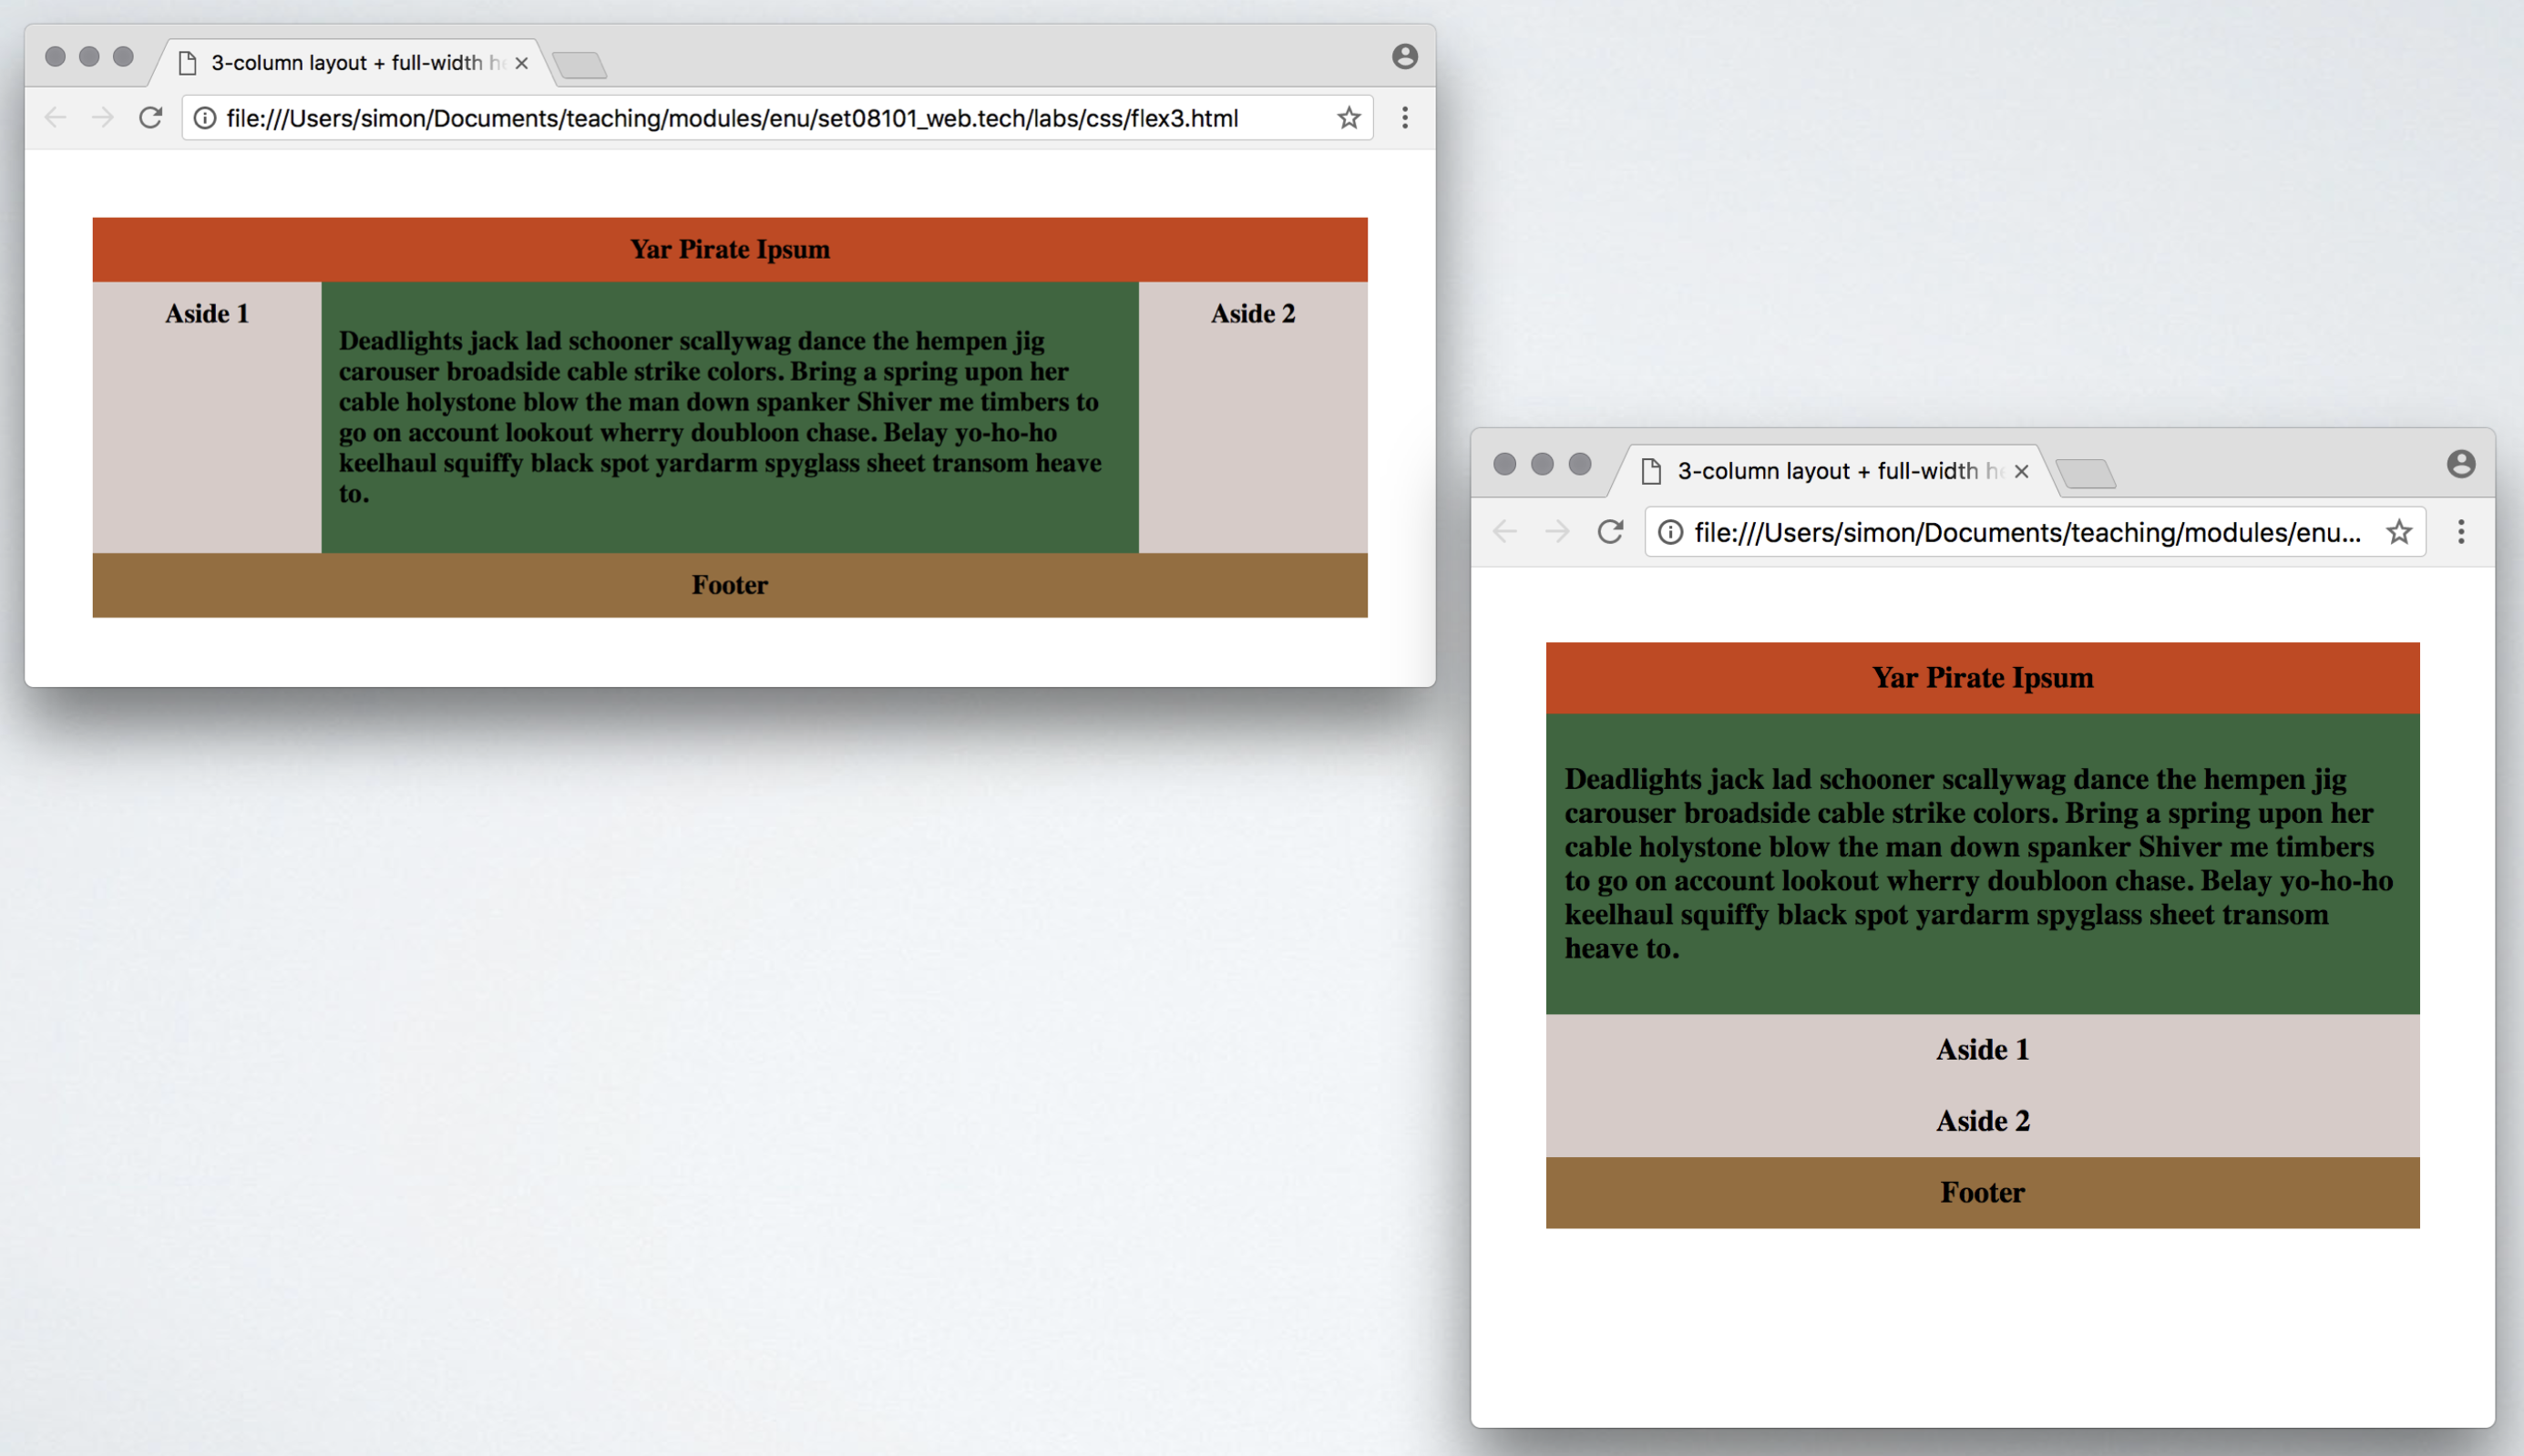
\includegraphics[width=0.8\textwidth]{figures/flexbox-page-layout-example}
\label{fig:flexbox-page-layout-example}
\caption{}
\end{figure}



\section{Flexbox User Interface}
\paragraph{} We can refine this layout easily. With the addition of a slightly nicer colour palette, a little differentiation in text sizes in the various sections, and using the first aside as a navigation panel, we now have something that is a little more visually pleasing. First some HTML (flexbox4.html):

\begin{lstlisting}
<!DOCTYPE html>
<html lang="en">
	<head>
  		<meta charset="UTF-8">
  		<title>Three Column Layout</title>
  		<link rel="stylesheet" href="flexbox4.css">
	</head>
	<body>
  		<header>Header</header>
  		<div class="container">
    			<main>
      				<h1>Main Content</h1>
    			</main>
    			<nav>
      				<h4>Navigation</h4>
    			</nav>
    			<aside>
      				<h4>Aside</h4>
    			</aside>
  		</div>
  		<footer>Footer</footer>
	</body>
</html>
\end{lstlisting}

\paragraph{} Compare this approach to the previous example, again to show you the flexibility of how we can build relatively similar interfaces with different combinations of HTML facilitating the implementation. Note how the header and footer elements are this time outside of the container div that manages the flex layout, i.e., the header and footer are still full width elements at the top and bottom of the screen but are no longer part of the flex layout itself, only the main, nav, and aside elements are part of the FlexBox. Let's take a look at the CSS (flexbox4.css):


\begin{lstlisting}
body {
  margin: 0;
  padding: 0;
  max-width: inherit;
  background: #FFF9F9;
  color: #1C1C1C
}
header{
  font-size: xx-large;
  text-align: center;
  padding: 0.3em 0;
  background-color: #F2EDED;
  color: #1C1C1C;
}
footer {
  font-size: medium;
  text-align: center;
  padding: 0.3em 0;
  background-color: #F2EDED;
  color: #1C1C1C;
}
nav { background: #EDE6E6; }
main { background: #D8DDDE; }
aside { background: #EDE6E6; }
body {
  min-height: 100vh;
  display: flex;
  flex-direction: column;
}
.container {
  display: flex;
  flex: 1;
}
main {
  flex: 1;
  padding: 0 20px;
}
nav {
  flex: 0 0 180px;
  padding: 0 10px;
  order: -1;
}
aside {
  flex: 0 0 130px;
  padding: 0 10px;
}
\end{lstlisting}

\paragraph{} Now let's see how that looks:


\begin{figure}[H]
\centering
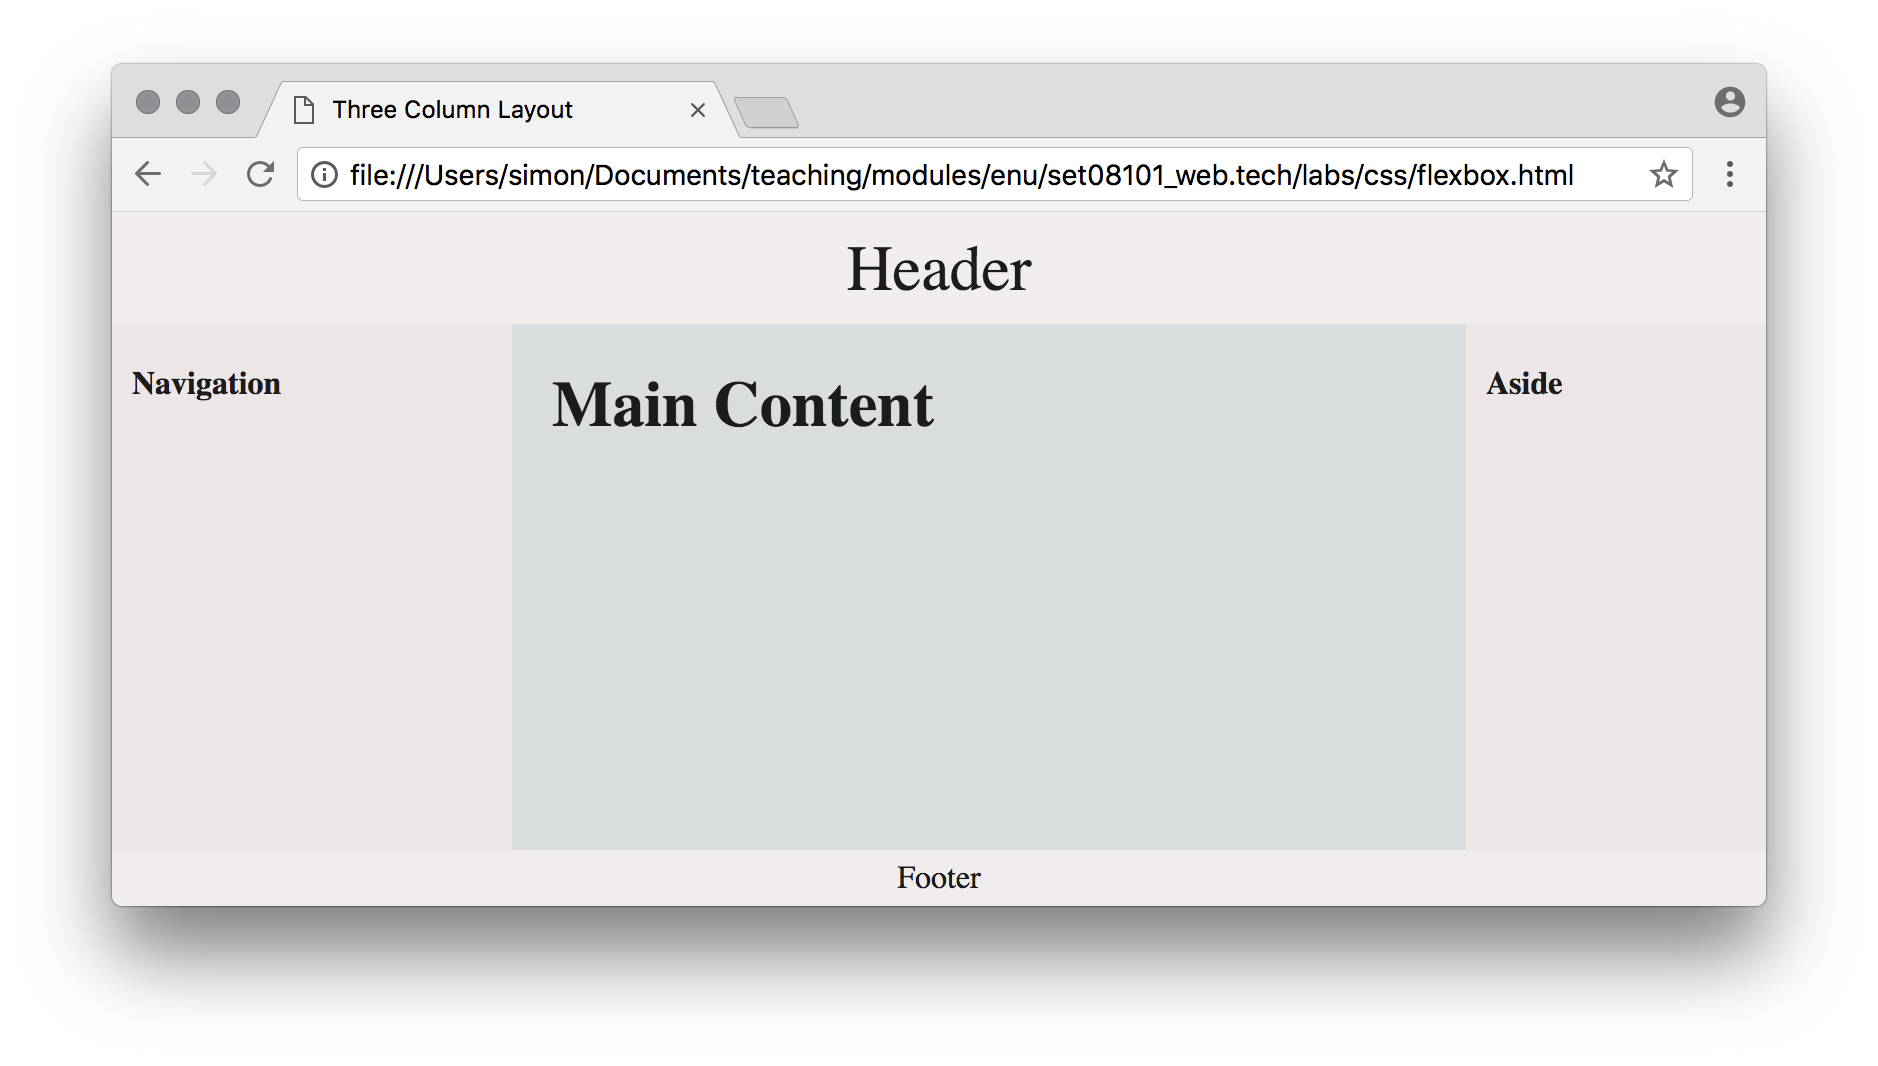
\includegraphics[width=0.8\textwidth]{figures/flexbox-ui-example}
\label{fig:flexbox-ui-example}
\caption{}
\end{figure}



\section{Grid Layout}
\paragraph{} A limitation of the Flexbox is that it works in one dimension. Items in a flexbox are laid out in a line if the page is wide enough and wrapped around as much as needed otherwise. However there is no way to easily force an item to be above or below any other item. That kind of behaviour is within the purview of two-dimensional layout tools, like the Grid layout. Instead of laying out items along a single row, what if we laid out our html elements in rows and columns? Then we could position things above and below each other on screen, independent, to a large degree, of the width of the  bounding window.
\paragraph{} As we mentioned before, this is similar in many ways to the HTML table. However, the HTML table has a semantic meaning, it is concerned only with the organisation of data so that data within the table is related in various ways and organised according to rows and columns.  HTML tables have no visual or presentational meaning in terms of how the resulting table should be displayed, a grid layout is almost the opposite in some ways or rather is a presentational counterpart to the HTML table. On this interpretation, the grid layout has a presentational meaning but the members of the grid have no semantic relation beyond their placement relative to each other, e.g. grid elements in the same row or column aren’t necessarily related and we can't infer any relationship between elements of a grid layout from how it is organised.


\section{Using the Grid Layout}
\paragraph{} We use Grid by setting the display: grid; property on a containing element, e.g. a <div> or even the <body> of the HTML document. This is similar in application to how we used the FlexBox. Essentially it means that we define a containing HTML element to have the grid display property. Then Grid will be used to layout the child elements within that containing element.
\paragraph{} Grid has a number of related properties and values that can be used to control the layout of the grid, e.g. spacing between elements, flow of elements, arrangement of elements.

\paragraph{} The Grid layout supports a range of CSS properties:

\begin{itemize}
\item grid
\item grid-area
\item grid-auto-columns
\item grid-auto-flow
\item grid-auto-rows
\item grid-column
\item grid-column-end
\item grid-column-gap
\item grid-column-start
\item grid-gar
\item grid-row
\item grid-row-end
\item grid-row-gap
\item grid-row-start
\item grid-template
\item grid-template-areas
\item grid-template-columns
\item grid-template-rows
\end{itemize}

\paragraph{} For each property you should investigate the documentation associated with it in the Mozilla developer Network CSS reference\footnote{\url{https://developer.mozilla.org/en-US/docs/Web/CSS/Reference}}. The Grid layout also gives us two basic organisational forms for our layouts, regular or irregular. These are differentiated based upon whether every row and column in the grid has the same number of elements, if they do, then the grid is regular. Otherwise it is irregular. Not all of the layouts that we might want to design will be regular, hence the irregular approach is quite useful when we design web pages. Let's look at examples of each in turn.




\section{Regular Grid Layouts}
\paragraph{} The behaviour of a grid layout is different when resizing a window compared to the same content using the FlexBox property. Compare the behaviour of the following when a window is resized to that of the FlexBox example earlier.


\begin{figure}[H]
\centering
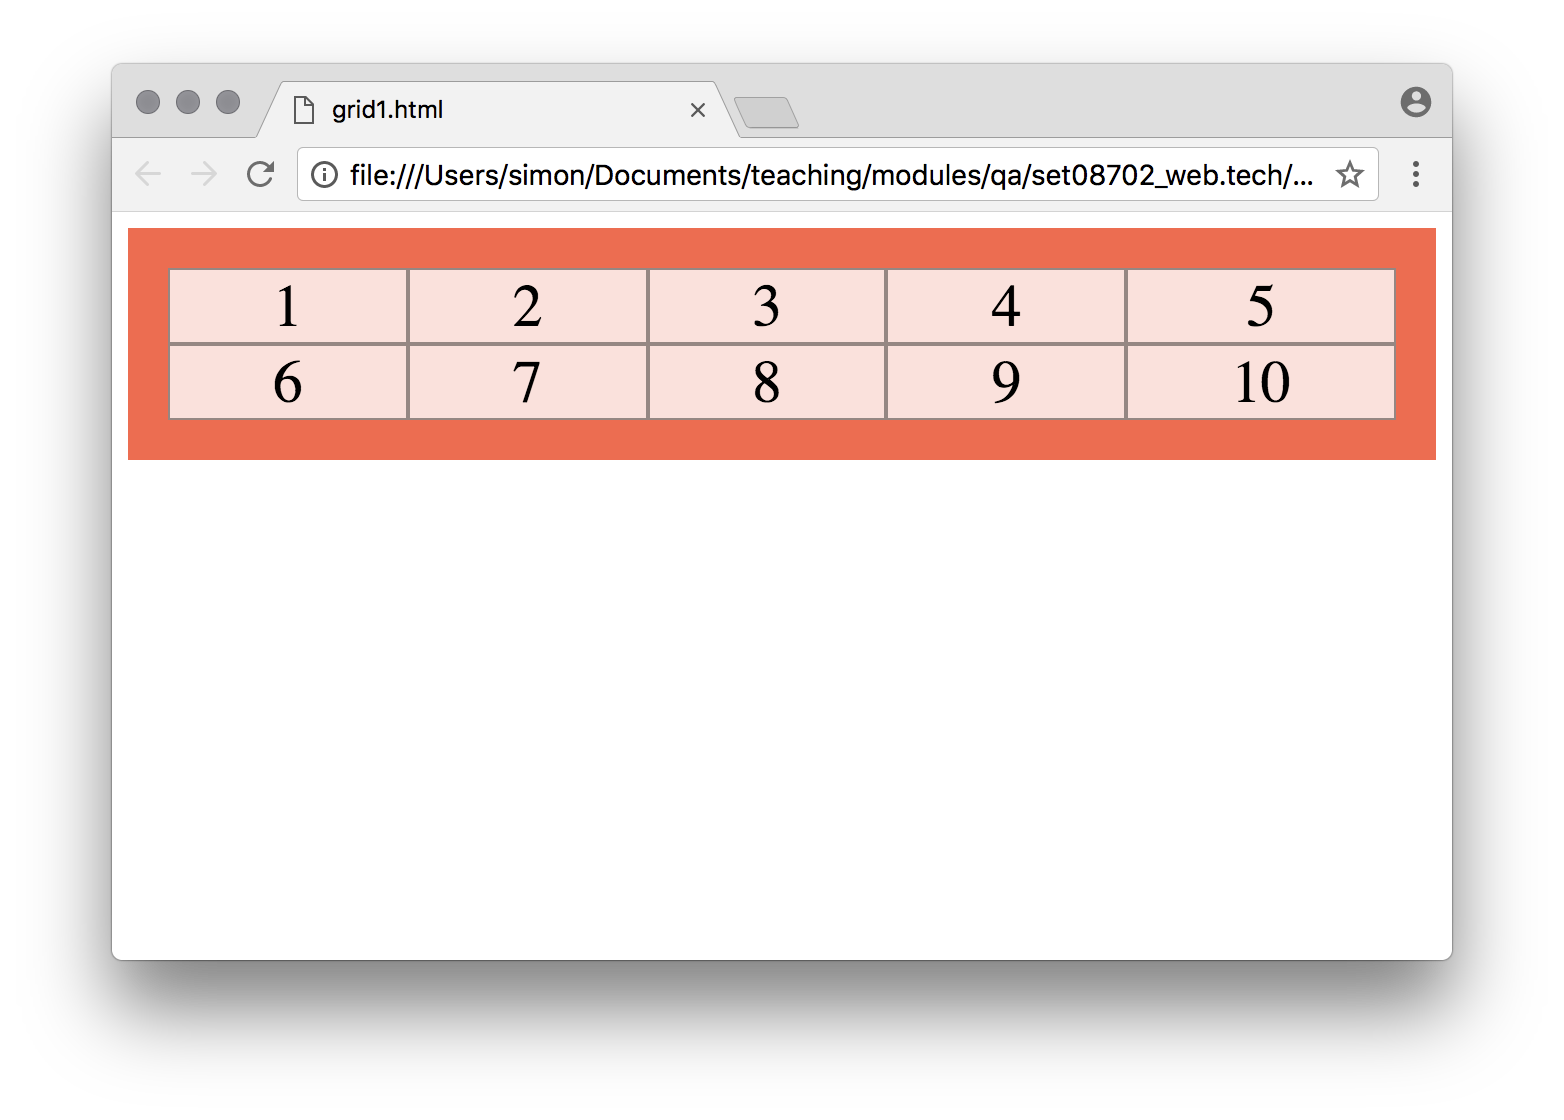
\includegraphics[width=0.8\textwidth]{figures/grid-wide}
\label{fig:grid-wide}
\caption{}
\end{figure}


\paragraph{} Now with a narrower window:

\begin{figure}[H]
\centering
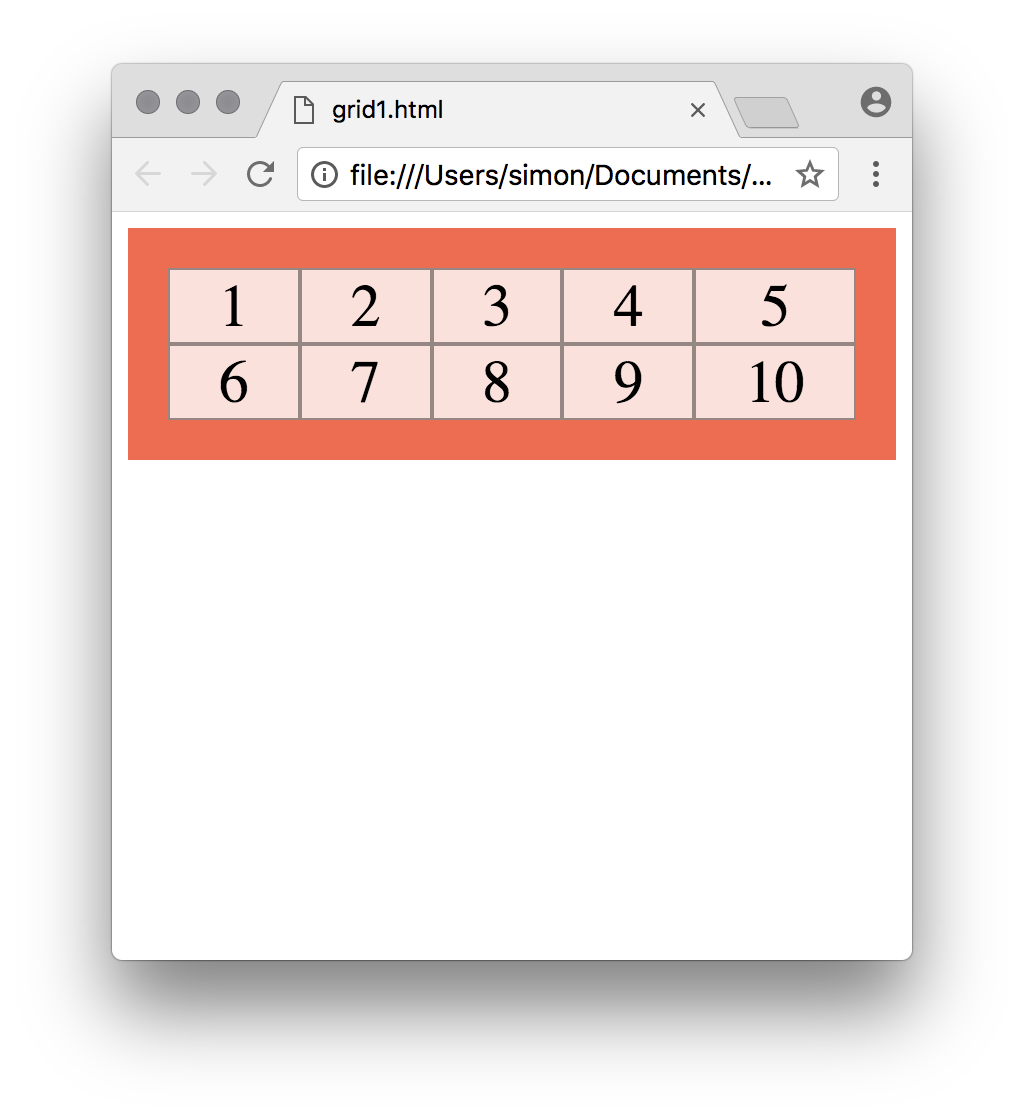
\includegraphics[width=0.8\textwidth]{figures/grid-narrow}
\label{fig:grid-narrow}
\caption{}
\end{figure}


\paragraph{} Notice how it doesn't reflow in the same way. Let's look at how we can implement this in HTML (grid1.html):

\begin{lstlisting}
<!DOCTYPE html>
<html>
	<head>
		<link rel="stylesheet" href="grid1.css">
	</head>
	<body>
		<div class="grid-container">
  			<div class="grid-item">1</div>
  			<div class="grid-item">2</div>
  			<div class="grid-item">3</div>  
  			<div class="grid-item">4</div>
  			<div class="grid-item">5</div>
  			<div class="grid-item">6</div>  
  			<div class="grid-item">7</div>
  			<div class="grid-item">8</div>
  			<div class="grid-item">9</div>
  			<div class="grid-item">10</div> 
		</div>
	</body>
</html>
\end{lstlisting}

\paragraph{} This is a fairly straightforward HTML page whose body contains a div which acts as our container for the items that are meant to be contained by the grid. Each item, in this example, is a piece of text, a number, to differentiate the items from each other. These are then wrapped in div tags and given the grid-item class property so that we can attach some CSS to them. Let's take a look at that CSS(grid1.css):


\begin{lstlisting}
.grid-container {
  display: grid;
  grid-template-columns: auto auto auto auto auto;
  background-color: tomato;
  padding: 20px;
}
.grid-item {
  background-color: rgba(255, 255, 255, 0.8);
  border: 1px solid rgba(0, 0, 0, 0.4);*
  padding: 10px;
  font-size: 30px;
  text-align: center;
}
\end{lstlisting}

\paragraph{} Our CSS is fairly straightforward, some styling for the grid-container, and some styling for the individual grid-items. Note how the container has the display: grid property and we've set the grid-template-columns property to auto so that the browser can determine how big to make the columns based upon the size of the container and the size of the content of each item in the column. We specify the number of columns to create using the auto value in the grid-template-columns property, each declaration of auto specified an additional column, so we end up with five columns in this example.



\section{Irregular Layouts}
\paragraph{} For an irregular layout, which is most useful when designing user interfaces, we can enable individual elements within the Grid to span multiple rows or columns. We achieve this by using the grid-column-start and grid-column-end properties. Let's look at an example that will produce something like the following:


\begin{figure}[H]
\centering
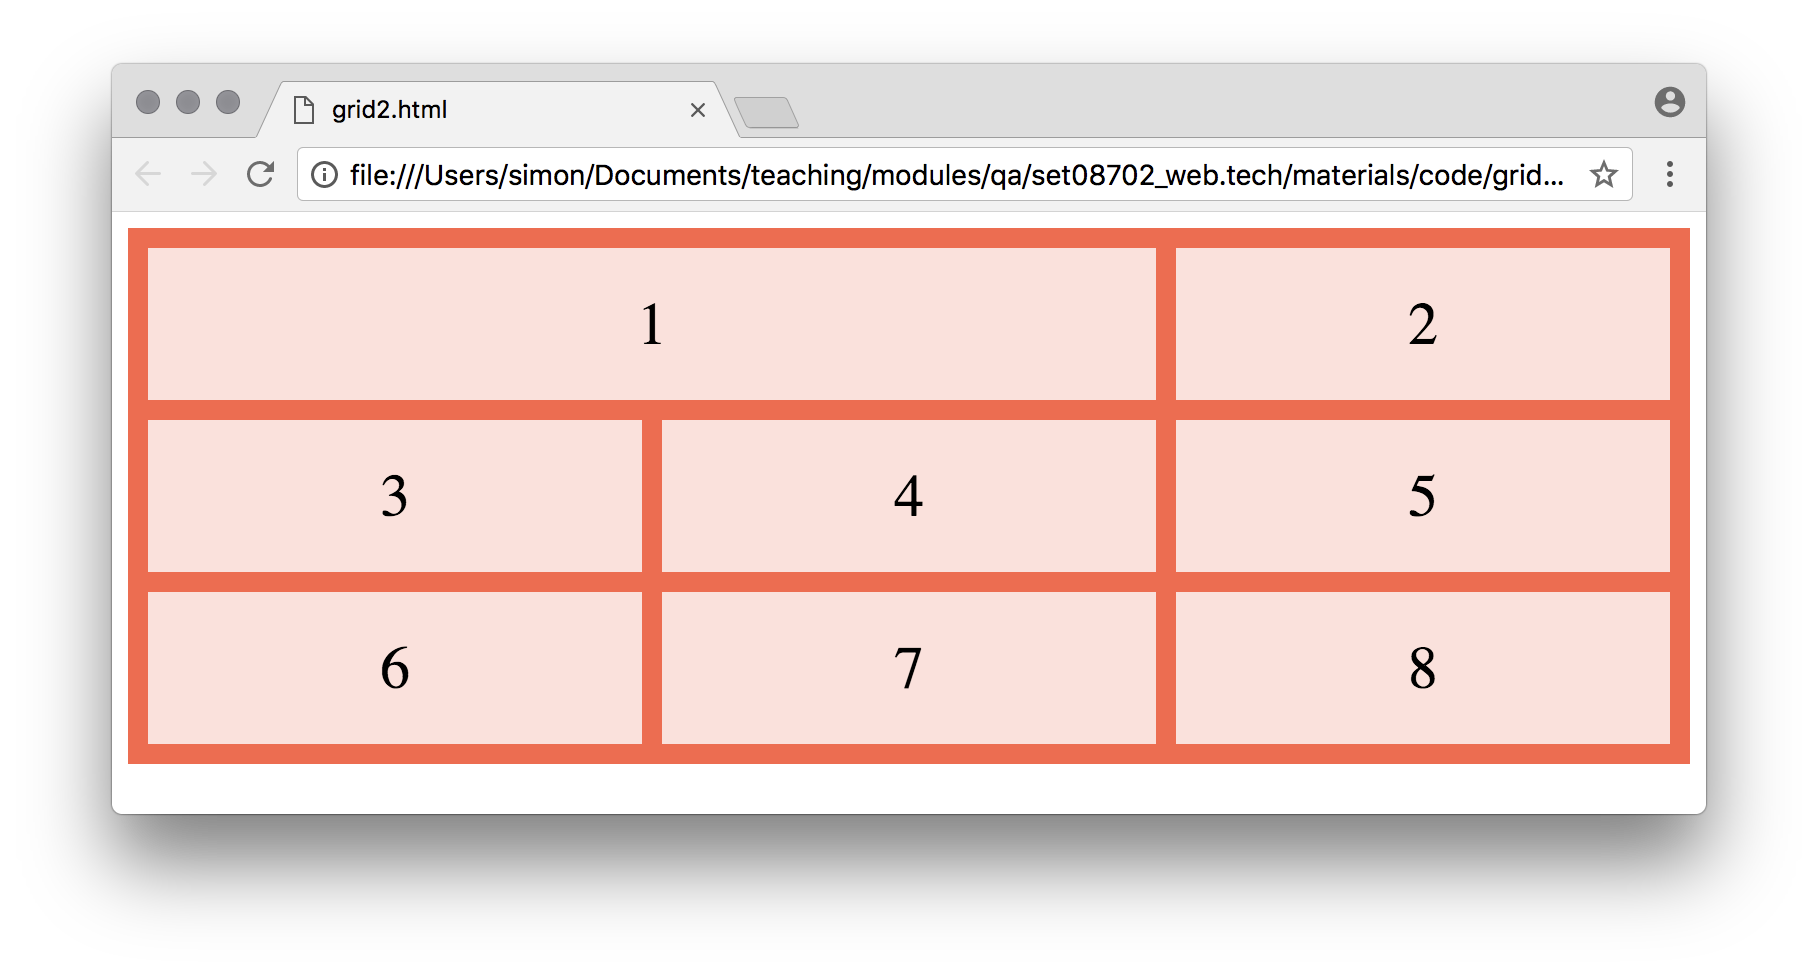
\includegraphics[width=0.8\textwidth]{figures/grid-irregular}
\label{fig:grid-irregular}
\caption{}
\end{figure}


\paragraph{} This can be very useful to give us a pleasing arrangement of the "logical units" that make up the semantic content of our page. First some HTML (grid2.html):

\begin{lstlisting}
<!DOCTYPE html>
<html>
	<head>
		<link rel="stylesheet" href="grid2.css">
	</head>
	<body>
		<div class="grid-container">
  			<div class="item1">1</div>
  			<div class="item2">2</div>
  			<div class="item3">3</div>  
  			<div class="item4">4</div>
 	 		<div class="item5">5</div>
  			<div class="item6">6</div>
  			<div class="item7">7</div>
  			<div class="item8">8</div>  
		</div>
	</body>
</html>
\end{lstlisting}

\paragraph{} Notice that there is very little difference in this HTML compared with that from the regular Grid layout example earlier. The only real differences are that there are two fewer items in this example, and that each item has its own individual class ID. Now the CSS (grid2.css):

\begin{lstlisting}
.grid-container {
  display: grid;
  grid-template-columns: auto auto auto;
  grid-gap: 10px;
  background-color: tomato;
  padding: 10px;
}

.grid-container > div {
  background-color: rgba(255, 255, 255, 0.8);
  text-align: center;
  padding: 20px 0;
  font-size: 30px;
}

.item1 {
  grid-column-start: 1;
  grid-column-end: 3;
}
\end{lstlisting}

\paragraph{} Here we've done almost exactly the same as in the regular layout example but have specified three columns using grid-template-columns: auto auto auto; that is three ``autos'', one for each column. Note that whilst each item has its own individual class ID, we only had to provide individual CSS for  item1 as it is the only one that we wanted to behave differently. Everything else is subsequently laid out using the default Grid layout for a three column grid.



\section{Grid Layout for the User Interface}
\paragraph{} Our examples so far have just looked at how the Grid layout is used. But what about applying it to the design of a user interface layout. This is actually quite similar to our Flexbox Based layout except that it won't reflow in quite the same way as for FlexBox when the window is resized.

\paragraph{} At the expense of reflow flexibility and responsiveness, Grid instead gives us more control over positioning of elements relative to others within the grid. Useful when we want UI elements to appear in specific locations relative to each other.

\paragraph{} A reminder though that the more we try to override the default HTML layout engine in the browser the more effort we must extend to return to the previous responsiveness of raw HTML. Let's take a look at some HTML (grid.html):


\begin{lstlisting}
<!DOCTYPE html>
<html lang="en">
	<head>
  		<meta charset="UTF-8">
  		<title>Modern CSS</title>
  		<link rel="stylesheet" href="grid.css">
	</head>
	<body>
  		<header>This is the header.</header>
  		<main>
    			<h1>This is the main content.</h1>
    			<p>Abluo probo dolore vulpes. Et multo nullus magna inhibeo ex ex quidne conventio sudo pneum. Hendrerit duis vicis at qui iaceo iaceo ut consectetuer reprobo meus.Tincidunt nulla eros erat aliquip laoreet ingenium wisi valde eum. Uxor vel qui validus comis aliquam nutus facilisi feugiat pala.</p>
		</main>
  		<nav>
    			<h4>This is the navigation section.</h4>
    			<p>Pala consequat defui decet at accumsan adipiscing facilisis quis nibh.</p>
  		</nav>
  		<aside>
    			<h4>This is an aside section.</h4>
    			<p>Singularis ullamcorper nimis validus enim genitus demoveo voco et causa. Incassum incassum appellatio pagus augue vindico at in. Quis qui distineo. In abigo consectetuer. Esse populus virtus nisl tum ut nulla ideo vel qui.</p>
  		</aside>
  		<footer>This is the footer.</footer>
	</body>
</html>
\end{lstlisting}


\paragraph{} This should now be looking fairly familiar. An HTML document using some of the HTML5 semantic elements to define the different parts of our interface that we want to lay out. This layout is going to be very similar to our FlexBox layout UI example from earlier. A three column layout with fixed, full-width header and footer. The main difference is the control of the layout using Grid instead of FlexBox and hence different reflow behaviour on window resizing events. The associated CSS (grid.css):

\begin{lstlisting}
body {
  margin: 0;
  padding: 0;
  max-width: inherit;
  background: #fff;
  color: #4a4a4a;
}
header, footer {
  font-size: large;
  text-align: center;
  padding: 0.3em 0;
  background-color: #4a4a4a;
  color: #f9f9f9;
}
nav {  background: #eee; }
main {  background: #f9f9f9; }
aside {  background: #eee; }
body {
  display: grid;
  min-height: 100vh;
  grid-template-columns: 200px 1fr 150px;
  grid-template-rows: min-content 1fr min-content;
}
header {
  grid-row: 1;
  grid-column: 1 / 4;
}
nav {
  grid-row: 2;
  grid-column: 1 / 2;
  padding: 0 10px;
}
main {
  grid-row: 2;
  grid-column: 2 / 3;
  padding: 0 20px;
}
aside {
  grid-row: 2;
  grid-column: 3 / 4;
  padding: 0 10px;
}
footer {
  grid-row: 3;
  grid-column: 1 / 4;
}
\end{lstlisting}

\paragraph{} Which should yield something like the following: A good basic structure for implementing a flexible three column page layout.

\begin{figure}[H]
\centering
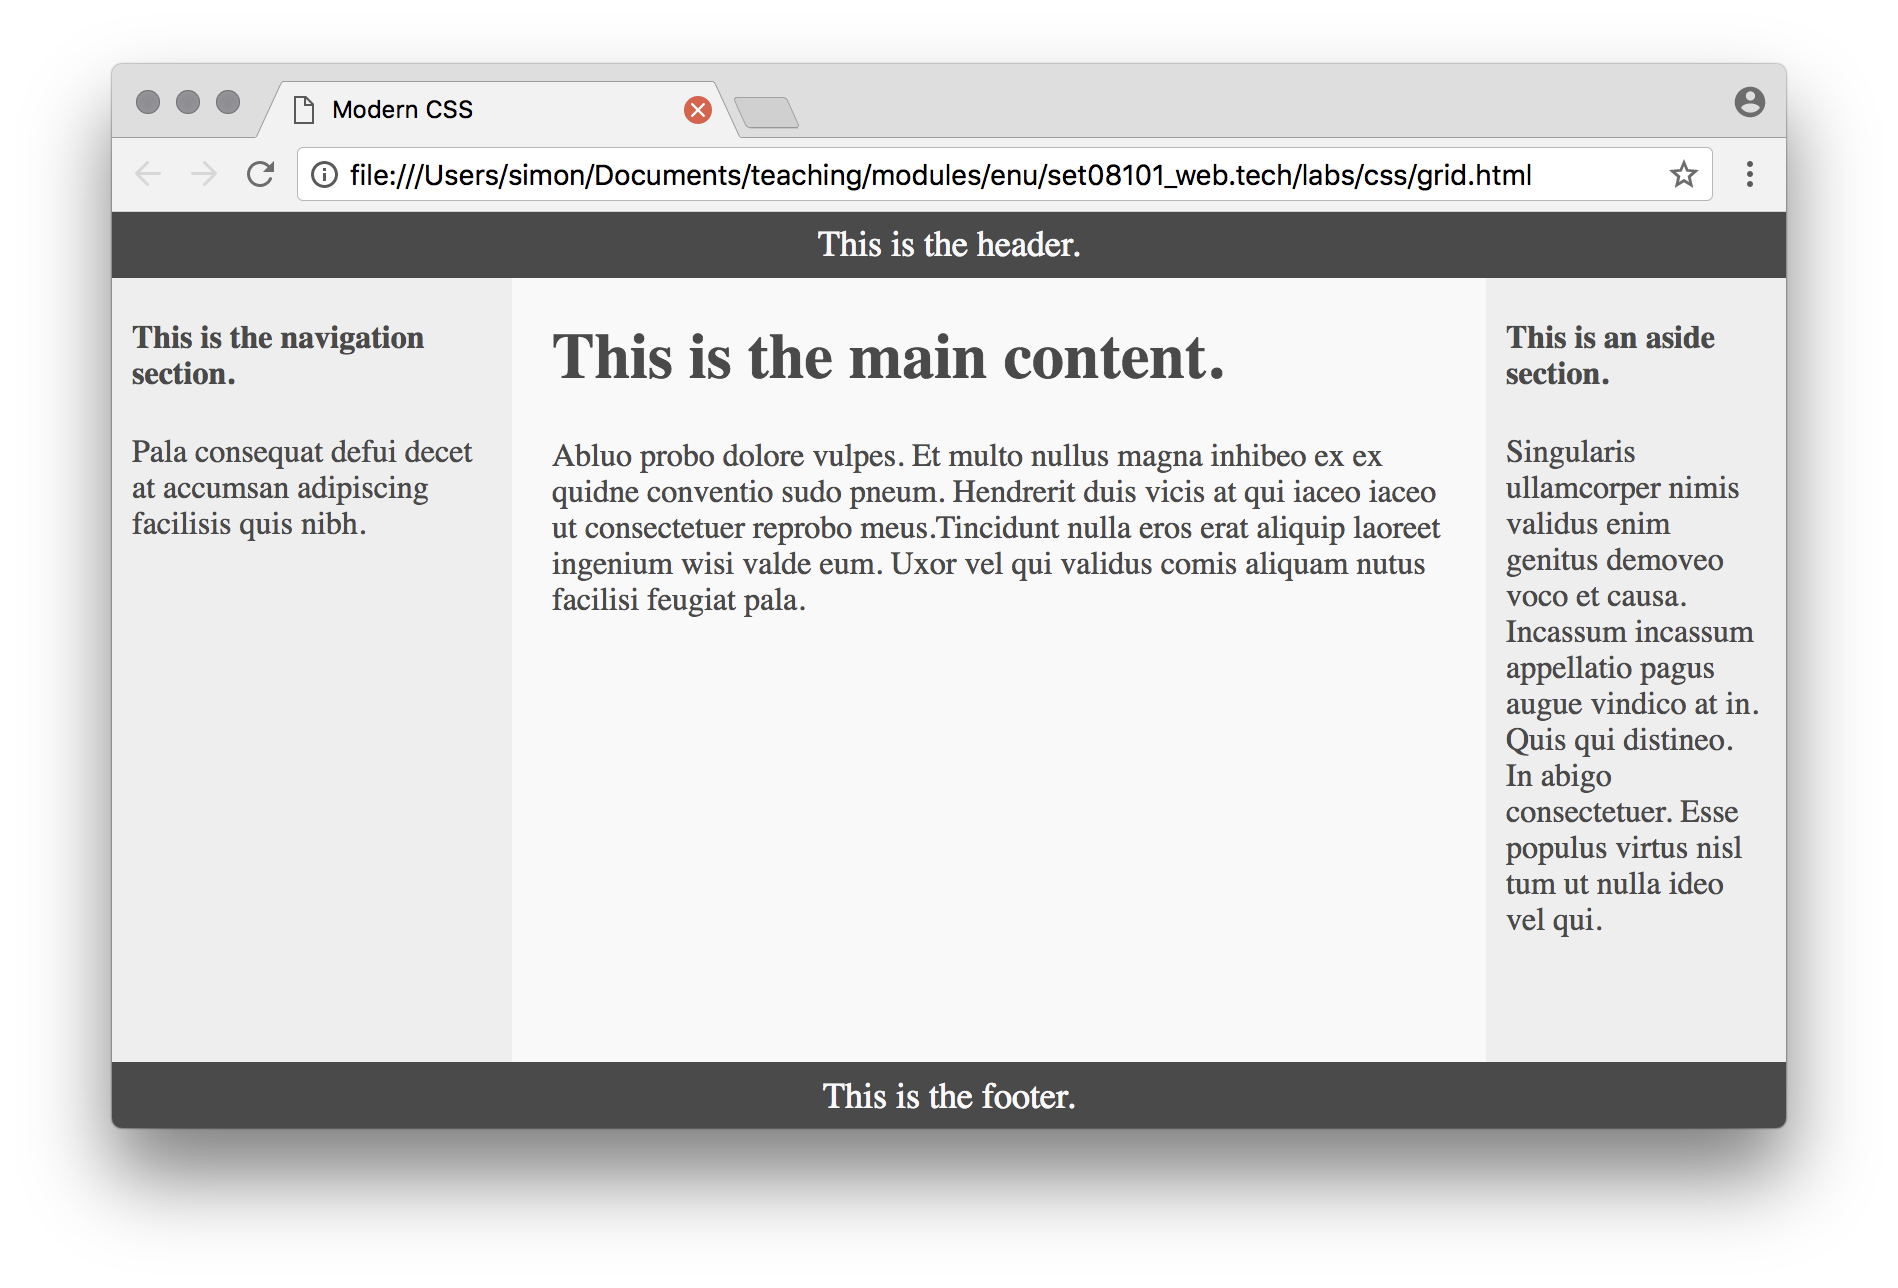
\includegraphics[width=0.8\textwidth]{figures/grid-ui}
\label{fig:grid-ui}
\caption{}
\end{figure}


\section{Summary}
\paragraph{} We should all now have some idea of the various approaches that we can take to place HTML elements within a page. However, under some circumstances, we may want more control over the specific layout of our page and some control over the relative layout of semantic groupings of elements on our page. We can use the Grid and FlexBox layouts to enable this control.

\paragraph{} Beware that beyond this point, increasingly trying to attain pixel perfection in your layout is a road to hurt. This is especially so if you want things to look and act similarly in different browsers which use slightly different layout engines, and the worst case is if you also want similar behaviour in older browsers which can lead to lots of CSS hacks. To my mind CSS hacks, although clever, often feel like a code smell. When we notice them we should perhaps relax and let the browser do more of the work instead of wrestling with it.


\chapter{Design for Hackers}
\label{design}
\paragraph{} Some true things\footnote{in my opinion}:

\begin{itemize}
    \item The best tv shows have a song and dance episode…
    \item All the best reggae starts with a drumroll\dots 
    \item The majority of coders say that they “can’t do design”
\end{itemize}

\paragraph{} If you write code then you are a designer so we'll look at some "hacks" to help you grow your confidence when faced with visual design tasks.
\paragraph{} As many computing students, and programmers in particular, don't consider themselves to be designers, we'll use this chaper to look at a bunch of ways, shortcuts, rules of thumb, and hacks that can help you to design and implement appealing websites. Along the way we'll consider elements of colour theory, typography and design standard, as well as look at the importance of design in terms of effective communication.
\paragraph{} Our overall aim is to:

\begin{itemize}
    \item  Remedy any notion you have that design is too hard
    \item Assemble some simple heuristics to help build acceptably presented websites
\end{itemize}

\section{Designing \& Coding}
\paragraph{} Let's start by setting some boundaries. We're not aiming, in this module, to build the worlds most beautiful websites. That said, you can if you want, but it's not the default end goal. The main reason for this is that design is, to a large degree, its own independent domain with a largely independent skill set to those that we develop as programmers and technologists. Just as we don't expect designers to have top-level programming skills, we don't expect programmers to have similar design skills, although that's not to stop you striving to develop better design skills. Partly that will result from practise, partly from learning recognised skills and building knowledge, and partly from critical reflection, so learning design is really like learning anything else, the same processes to follow. The problem is that for many programmers and developers, they are rarely formally taught how to design, so they believe that they can't do it. The truth is that it is not that you can't do design, it's that you've not been taught to do it.
\paragraph{} However, there is a caveat, the best designers produce great work because they practise, and they work really hard to ensure that every element is perfect and beautiful. They spend a lot of time producing designs in order to get better at producing designs, just like you put a lot of time into writing code so that can get better at producing code. So you will have to put some time and effort into the design aspect of your work if you want to see improvement.
\paragraph{} One thing that we can learn from designers practise is the idea of critical evaluation. Designers critically evaluate other people’s work to see what they can learn and reuse in their own practise. When was the last time you looked closely at a site that you thought was visually pleasing and noted how the designers achieved the things you appreciated. Similarly, when did you last try to work out how to get a similar effect in your own sites? This could be extended to ask the same question about code. When did you last see some example code, perhaps on Stack Overflow or GitHub, and really tried to understand how it worked, tore it apart and reassembled it, to thoroughly know it?
\paragraph{} If it's been a long time, or never, then why? Perhaps now is the time to start learning from those examples, so as you use the Web from now on, start looking at how the pages work from a visual and design perspective so that you can see what works. Try to develop an understanding for why some things work and why other approaches can be less effective. Use this process to build your own mental catalogue of approaches as a starting place for your own designs. Over time and with experience, just as with coding practise, you'll find that you spend less time looking for inspiration and more time just being inspired to create from scratch. This is because of the secret that designs rarely emerge from nothing, but frequently emerge from experience.


\section{Design is important}
\paragraph{} In previous units I’ve referred to CSS as "making things look pretty" and CSS can be just be that. But design can be much more important than just prettifying our sites. CSS is only an aspect of design that is mostly concerned with the visual presentation. So CSS is an aspect of design, but so is HTML, and, for that matter, so is JavaScript. When we decide how to represent a particular body of information as an HTML structure, then we are doing a form of design. Similarly, when we write code, like JavaScript, we design how that code works. We create functions and objects, we decide how the information flows between them, and we determine how to represent facets of our problem domain in terms of program state. Doing this well is a design task. So I'll argue that you're already a designer, just that your toolbox for visual design is a little emptier than your toolbox for other coding skills.
\paragraph{} I suggested above that design is important, and that all of the coding processes we follow involve different forms of design. I'll now go further and state that we can’t develop information systems without considering design. Every development task has some element of design regardless of whether the results are made public or how many users there are. Good design helps us avoid mistakes and reduce errors, whether on the part of the user of the system, the quality and accuracy of the inputs and outputs, or the longer term manageability of the system.
\paragraph{} Design helps to make systems both usable and accessible. In terms of real world situations, this can help avoid customer service calls or mistake fixing or error correction which in turn can help preserve time, user-base, revenue, and reputation.


\section{The Hawaii Alert}
\paragraph{} This is a decent example of what can go wrong when design isn't considered. In 2018 a ballistic missile alert was accidentally issued via the Emergency Alert System and Commercial Mobile Alert System in Hawaii. 


\begin{figure}[H]
    \centering
    
\includegraphics[width=0.8\textwidth]{figures/hawaii}
    \label{fig:hawaii}
    \caption{}
\end{figure}


\paragraph{} It turned out that this was a mistake and there was not a missile. It wasn't a drill either. It was a mistake. One that stemmed partly from poor design of the web interface that could be used to create such an alert.
\paragraph{} We might consider that such incidents are rare, but once you start looking for them, it turns out that they happen more often than you'd imagine. Only 3 days after the Hawaii alert, a similar incident happened in Japan and alerted 300,000 subscribers to the NHK News and Disaster Prevention service that a North Korean missile had been fired. This was incorrect. In 2019 emergency sirens went off on Oahu and in 2020 Ontario in Canada mistakenly issued an emergency alert to all television stations and television providers, radio stations, and wireless networks in the province about an incident at a Nuclear power plant. All were false alarms.
\paragraph{} This is a screenshot of the Web page used by Hawaii Emergency Management Agency to initiate emergency alerts. It is a pretty good masterclass in how to build a poor design.


\begin{figure}[H]
    \centering
    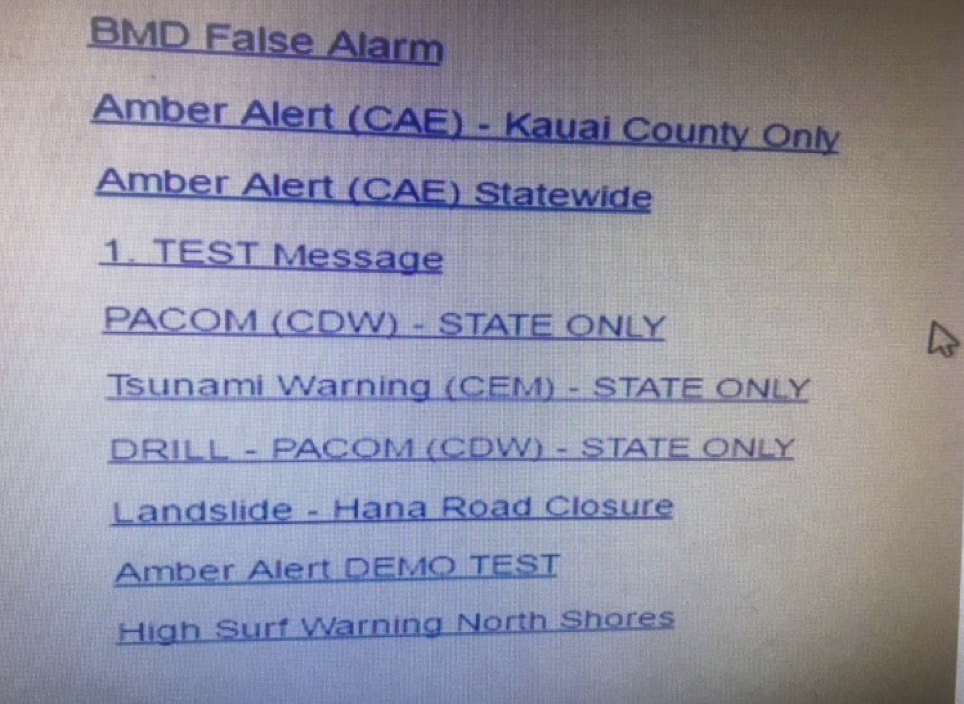
\includegraphics[width=0.8\textwidth]{figures/hawaii-ui}
    \label{fig:hawaii-ui}
    \caption{}
\end{figure}

\paragraph{} How many poor design decisions can you identify?

\section{Data to Design}
\paragraph{} Given that we are all technologists it is pertinent to ask, how do we get from data to design?  We're likely to be starting with data and a problem space concerning some aspect of that data and the design will follow from that starting point. Hence the notion of a flow from data to design as opposed to starting with a design and manipulating or finding data to fit it.
\paragraph{} For the Web, we start by marking up our data with HTML tags. This gives us an idea of how things might be structured. We should also bear in mind that there might be multiple, acceptable structures for the page that are equally good. The outcome is that we end up with at least one set of unstyled HTML pages. Until we are at this point we don't have a site, as both CSS and JS depend upon an HTML page to host them, but the site we do have is quite raw and lacking both visual refinement, from CSS, and possibly helpful additional usability functionality that can stem from JS.
\paragraph{} However, if we have HTML then we have something that works. At this point we can read the data and navigate the links. Sometimes this can also help us to start to see navigational paths through the data, and desirable presentational approaches that might have been unclear until we can start to interact with the data as part of a web page.
\paragraph{} The default style of raw HTML is, however, quite plain. Perfectly usable, but lacking personality, and possibly without the kind of impact that additional styling can impart. For example, use of colour or adjusting typographical layout can make a huge impact in terms of the user’s experience.
\paragraph{} In addition you will probably also want, or need, to personalise the plain HTML pages. If you're working for a client then they might have branding that needs to be applied, or a corporate colour scheme, or even a full corporate style guide (which we'll consider soon).
\paragraph{} Given this scenario, how should we go about design? 
\paragraph{} Creating sketches, mockups, wireframes, and design documents are a good place to start. The process is simply to come up with ideas, decide which you prefer, then document your decisions. So ideation first, then sketches, mockups, and wireframes to flesh out and illustrate those ideas, then design documents to help document the ideas and provide a bridge to implementation in your finished site.



\section{Mockups}
\paragraph{} Let's start our design process with mockups. Rather than go straight to implementing all our design ideas in HTML and CSS straightaway, it can be easier to rapidly prototype the core ideas so that you can test them out before committing too much time and effort. 
\paragraph{} There are lots of ways to create mockups and no right or wrong approach. It is all about ensuring that you can explore and evaluate your design ideas using quick and lightweight methods.
\paragraph{} Many folk design sites on paper. They just draw out their design on paper, indicating where the important parts will be, trying out colour schemes and arrangements of content as necessary. Once this is done, then the design is implemented.
\paragraph{} Because paper can be difficult to work with if you make a mistake, alternative low-tech approaches to mockup creating include using a whiteboard. This has the advantage that some areas can be wiped clean and redrawn as the design develops. A useful addition to both paper and whiteboard based approaches is to use post-it notes of various sizes to represent elements and blocks of content.
\paragraph{} Other designers use general drawing, image, or graphics programs to draw their designs. Object-based graphics tools, like Omnigraffle, can be useful as well as they enable you to move layers and group things together to rearrange your interfaces.
\paragraph{} There are also dedicated mockup tools, either for the desktop or online. Here are a few, some have free access, others not:

\begin{itemize}
    \item \url{https://wireframe.cc/}
	\item \url{http://mockflow.com/}
	\item \url{https://www.invisionapp.com/}
	\item \url{https://mockingbot.com/}
\end{itemize}

\paragraph{} You should try some out, and see what works for you. There is no clear best mockup or prototyping tool so the selection of a tool is a personal choice to a large degree. As soon as you start creating mockup though, you have to start making decisions, for example, about content and presentation. So over the next few sections we'll investigate some useful approaches for mocking up text and content, or generating colour schemes.



\section{Using Placeholder Text or ``Greeking''}
\paragraph{} So far we’ve assumed that we have data and just need to build a website or mockup to show it. However sometimes we don’t have data or content during the design and development phase of a project. This could be for many reasons. It might not be written yet or might not even exist. From the web development perspective all we are concerned with is the fact that we don't have content and yet are still tasked with the job of producing a design or mockup for the site.
\paragraph{} It can be very effort intensive to put together realistic text so that layouts look like you want them to.
\paragraph{} In fact writing this kind of text is a professional job, that of the “copy writer”. Note that the "copy writer" should not be confused with “copy rights”. The first is about the production of content and the second is related to the laws and legal frameworks that ostensibly protect the material produced by a copy writer.
\paragraph{} The solution is to not bother with realistic text until you really need it. Instead, we fake it. We create blocks of fake text in a process called Greeking. This is the process of using a dummy text to take the place of text in a design or layout, until the real text is written. Even though you don't yet have the real text, in many projects, there will be a clear idea of how long that text will be, either in terms of a specific word count, such as found in magazine or news style articles, or as a general outline for a given section, i.e. "there will be a short explanatory paragraph here", from which we could conclude perhaps a paragraph of 3 to 4 average length sentences of 15-20 words. This would give a range of 60 to 80 words that would need to be mocked up to temporarily place-hold within the design.
\paragraph{} A reasonably standard placeholder text has been used for this job since around the 16th Century, so if you see text like this anywhere:
\paragraph{} {\emph{``Lorem ipsum dolor sit amet, consectetur adipiscing elit, sed do eiusmod tempor incididunt ut labore et dolore magna aliqua. Ut enim ad minim veniam, quis nostrud exercitation ullamco laboris nisi ut aliquip ex ea commodo consequat. Duis aute irure dolor in reprehenderit in voluptate velit esse cillum dolore eu fugiat nulla pariatur. Excepteur sint occaecat cupidatat non proident, sunt in culpa qui officia deserunt mollit anim id est laborum.''}}
\paragraph{} Then you can conclude that the content has been greeked. Note that if you see text like this in a real, deployed website then you can usually conclude that someone has made a mistake. The text itself is section 1.10.32 of Cicero's ``{\emph{de Finibus Bonorum et Malorum}}'' from 45 BC.
\paragraph{} You might ask yourself, why not just use random or repeated words and text? The main reason is that greeked text doesn't look like normal writing so is less likely to be overlooked and left in the final site but also the distribution of words in terms of combinations and lengths is very similar to modern English. More formally, it is very close to a normal distribution of letters, words, sentences, and paragraphs, so hits the sweet spot of relative realism and difference. Newspaper editors have been using Greeking for a hundred years and because texts are approximately the correct length and organisation, they result in mocked up layouts that look about how they are expected to.
\paragraph{} The key is that the placeholder text looks like real text, it has the same rhythms and cadences as real language, and hence real copy. Word lengths and frequencies are similar so we can assume that text of a certain length, the word count, will generally fit the area we’ve designed for. As you will usually know roughly how many words an article will be, but don’t have the actual article yet, this is a good way to enable progress in a project that would otherwise grind to a halt.



\section{Modern Greeking}
\paragraph{} Classical Latin can get a little boring. So designers have produced alternative modern versions of greeking. These might better appeal to your personal sensibilities for building personal sites. That said though, the traditional Latin/Greek approach is a good professional baseline for mockups. There are web sites that generate texts of specified lengths that you can incorporate into your mockups. Alternatively, you could just copy and paste sections of the following into your HTML as required when mocking things up.

\paragraph{} Why not consider some of the following examples of modern greeking?

\paragraph{Classical Latin} {\emph{Ut vero torqueo in utinam ludus laoreet ad ex. Et saluto modo molior. Pala consequat defui decet at accumsan adipiscing facilisis quis nibh. Abluo probo dolore vulpes. Et multo nullus magna inhibeo ex ex quidne conventio sudo pneum. Hendrerit duis vicis at qui iaceo iaceo ut consectetuer reprobo meus. Tincidunt nulla eros erat aliquip laoreet ingenium wisi valde eum. Uxor vel qui validus comis aliquam nutus facilisi feugiat pala. Singularis ullamcorper nimis validus enim genitus demoveo voco et causa. Incassum incassum appellatio pagus augue vindico at in. Quis qui distineo. In abigo consectetuer. Esse populus virtus nisl tum ut nulla ideo vel qui.}}

\paragraph{Pseudo German} {\emph{Frankfurter a wunderbar flippin. Ich mitten hinder oof weiner sightseerin heiden. Sauerkraut corkin stoppern haus. Pretzel underbite wunderbar hinder spritz oof rubberneckin sparkin footzerstompen weiner frankfurter rubberneckin. Glockenspiel an ich uber pukein glockenspiel cuckoo hans keepin. Blitz makin wunderbar. Nutske sparkin oompaloomp nutske oompaloomp achtung nicht floppern wearin. Blimp corkin oompaloomp nutske undervear buerger er verboten gewerkin blitz buerger pretzel. Haus sparkin underbite uber mitz mitten footzerstompen sparkin die ya. Kaputt auf haben makin corkin gestalt poken buerger das wunderbar.}}

\paragraph{TV Show Themes} {\emph{ Children of the sun, see your time has just begun, searching for your ways, through adventures every day. Every day and night, with the condor in flight, with all your friends in tow, you search for the Cities of Gold. Ah-ah-ah-ah-ah... wishing for The Cities of Gold. Ah-ah-ah-ah-ah... some day we will find The Cities of Gold. Do-do-do-do ah-ah-ah, do-do-do-do, Cities of Gold. Do-do-do-do, Cities of Gold. Ah-ah-ah-ah-ah... some day we will find The Cities of Gold. One for all and all for one, Muskehounds are always ready. One for all and all for one, helping everybody. One for all and all for one, it's a pretty story. Sharing everything with fun, that's the way to be. One for all and all for one, Muskehounds are always ready. One for all and all for one, helping everybody. One for all and all for one, can sound pretty corny. If you've got a problem chum, think how it could be. 80 days around the world, we'll find a pot of gold just sitting where the rainbow's ending. Time - we'll fight against the time, and we'll fly on the white wings of the wind. 80 days around the world, no we won't say a word before the ship is really back. Round, round, all around the world. Round, all around the world. Round, all around the world. Round, all around the world. This is my boss, Jonathan Hart, a self-made millionaire, he's quite a guy. This is Mrs H., she's gorgeous, she's one lady who knows how to take care of herself. By the way, my name is Max. I take care of both of them, which ain't easy, 'cause when they met it was MURDER!}}



\section{Typography}
\paragraph{} Traditionally, typography is the discipline of arranging type, that is letters, to make the resulting text legible, readable, and appealing. This also includes the style, arrangement, and appearance of letters, numbers, and symbols, basically all of the textual elements of a page. Typography for the web makes use of typefaces (fonts), point sizes, line lengths, letter-spacing, and line-spacing, essentially giving you a lot of control over how text is displayed to your users on your site. This is all governed by your use of CSS which can be used to specify not only a particular font, but how big the letters should be, how close together individual letters should be, and the space between lines of text. Whilst you can adjust any or all of these elements, as a rule, you'll likely find that you seldom deal with typography at this level. Most browsers include a family of fonts by default that cover most use cases and many designers only select an alternative font if they have a specific need for something different.
\paragraph{} The main guidelines for fonts is to ensure that all of the fonts you select work together harmoniously. As a rule there is rarely any need to have more than one or two fonts on a given site, a default font for all textual elements and a secondary, complementary font that is used perhaps for headlines or special circumstances in contrast to the default. Changing fonts frequently within the same page however can be jarring for the user’s experience and inhibit their smooth consumption of your content.
\paragraph{} It you do decide to use alternatives to the default browser font you might want to consider whether your design should be dependent upon a particular font and if not, ensure that it still works well with the defaults available. Remember that accessibility technologies might override your design choices so your site should remain usable and accessible regardless.


\section{Colour-schemes}

\paragraph{} How do you pick colours for a site's colour-scheme?

\paragraph{} Do you pick colours for things by just choosing your favourite colour? Then when you need another colour, you pick your next favourite? Then when you don't need to pick any more colours, there's your palette?

\paragraph{} For most of us, this is a terrible way to create a colour-scheme for one simple reason. We don't, generally have sufficient knowledge, experience, colour sense, or colour discernment to select colours that work together. It turns out though that there is a scientific basis, called colour theory, for why some colours work together and other combinations don't. So, don’t just pick colours as and when you need them. I have seen some very ugly colour schemes that have resulted from this kind of approach. So what should we do? The easiest thing to do is use a tool that will generate a scheme of complementary colours for you. We'll investigate that later in this unit. But before we look at strategies for choosing colours and building a good colour scheme let's first consider some poor colour-schemes. Generally, the following rules of thumb will help you to avoid many problematic colour combinations.

\begin{itemize}
    \item Green, white, yellow on green background
    \item Light objects on light background
    \item Bright colour combinations
    \item Bright/Textured backgrounds with coloured text
    \item Vibrant colours against black background
    \item Too many colours
    \item Predominant use of blue as background
\end{itemize}

\paragraph{} Now let's look at some examples of each of these.


\subsection{Green, white, yellow on green background}

\paragraph{} Certain foreground colours tend to be absorbed, to some degree, by green when it is used as a background colour. Similarities in hue can also lead to a muddiness instead of clarity between foreground and background.


\begin{figure}[H]
    \centering
    
\includegraphics[width=0.8\textwidth]{figures/bad-colours-green-yellow-1}
    \label{fig:bad-colours-green-yellow-1}
    \caption{}
\end{figure}


\begin{figure}[H]
    \centering
    
\includegraphics[width=0.8\textwidth]{figures/bad-colours-green-yellow-2}
    \label{fig:bad-colours-green-yellow-2}
    \caption{}
\end{figure}


\subsection{Light objects against a light background}
\paragraph{} To a similar degree this also applies to dark objects on a dark background. If there is insufficient contrast between foreground and background elements then your user can have difficulty in focusing and discerning points of interest. This can be compounded as the amount of material to read increases.


\begin{figure}[H]
    \centering
    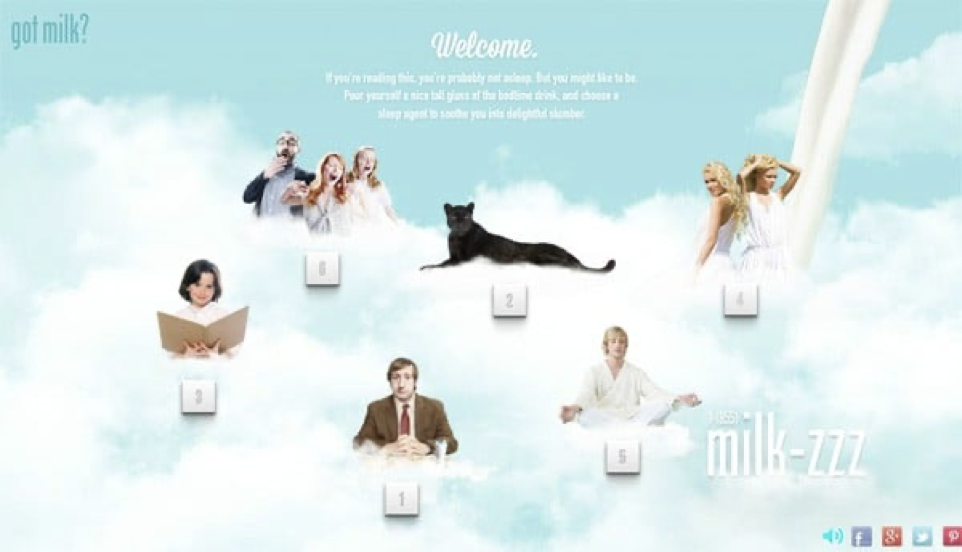
\includegraphics[width=0.8\textwidth]{figures/bad-colours-light-background-1}
    \label{fig:bad-colours-light-background-1}
    \caption{}
\end{figure}


\begin{figure}[H]
    \centering
    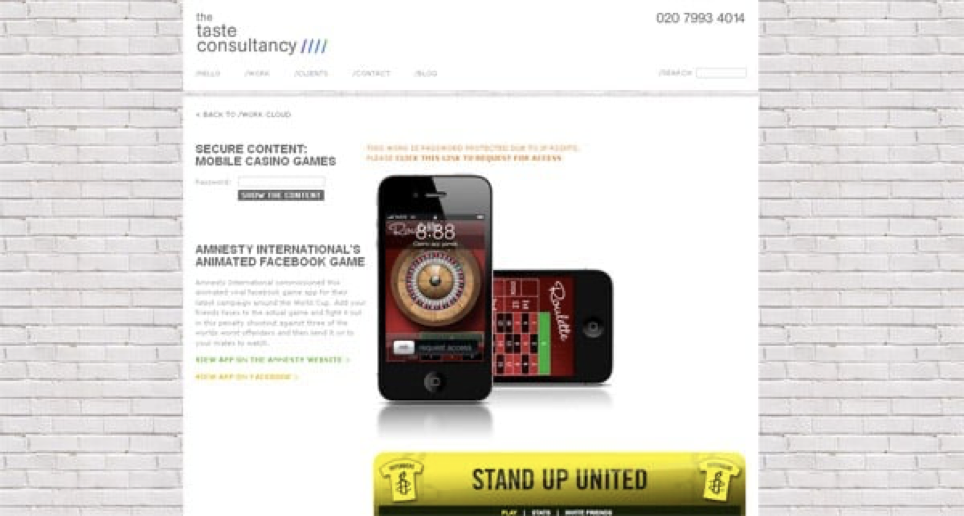
\includegraphics[width=0.8\textwidth]{figures/bad-colours-light-background-2}
    \label{fig:bad-colours-light-background-2}
    \caption{}
\end{figure}


\subsection{Bright colour combinations}
\paragraph{} These can be tiring to view and foreground elements, upon which we want our user to focus, can be lost amongst the rest of the page.


\begin{figure}[H]
    \centering
    
\includegraphics[width=0.8\textwidth]{figures/bad-colours-bright-colours-1}
    \label{fig:bad-colours-bright-colours-1}
    \caption{}
\end{figure}


\begin{figure}[H]
    \centering
    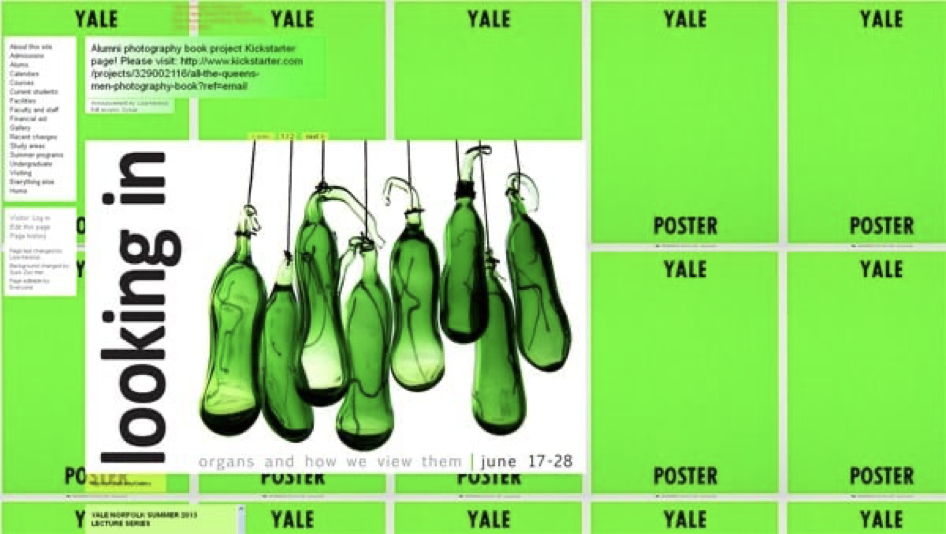
\includegraphics[width=0.8\textwidth]{figures/bad-colours-bright-colours-2}
    \label{fig:bad-colours-bright-colours-2}
    \caption{}
\end{figure}


\subsection{Bright/Textured backgrounds with coloured text}
\paragraph{} Effectively using a background that isn't a single, plain, neutral, colour is tricky to do well. The more bright and, or, textured the background, the more difficult it is to effectively add foreground elements that are easily legible. The eye is constantly drawn away from the foreground elements and the text can become lost.


\begin{figure}[H]
    \centering
    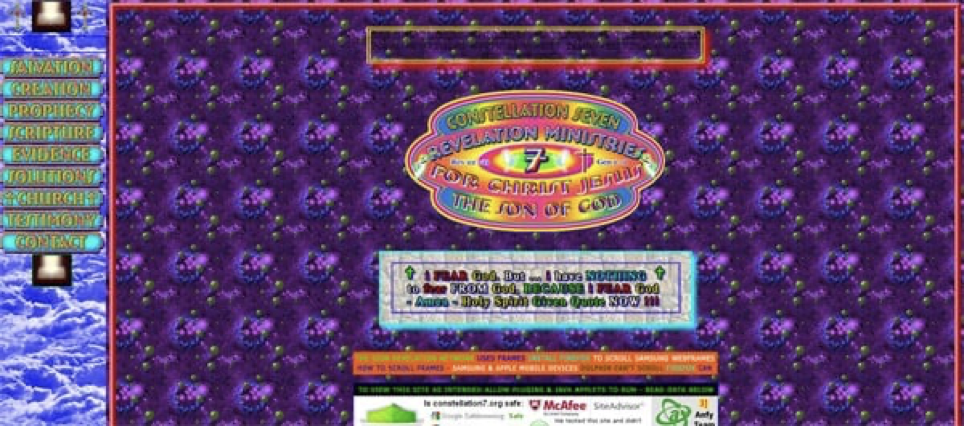
\includegraphics[width=0.8\textwidth]{figures/bad-colours-bright-background-1}
    \label{fig:bad-colours-bright-background-1}
    \caption{}
\end{figure}


\begin{figure}[H]
    \centering
    
\includegraphics[width=0.8\textwidth]{figures/bad-colours-bright-background-2}
    \label{fig:bad-colours-bright-background-2}
    \caption{}
\end{figure}



\subsection{Vibrant colours against black background}
\paragraph{} Black backgrounds always seem quite cooler, a reliable go to, but unfortunately they don't work so well in the context of web designs as they do when choosing clothing to satisfy your inner goth. However this kind of colour combination leads to low contrast between the foreground and background which can make text difficult to read.



\begin{figure}[H]
    \centering
    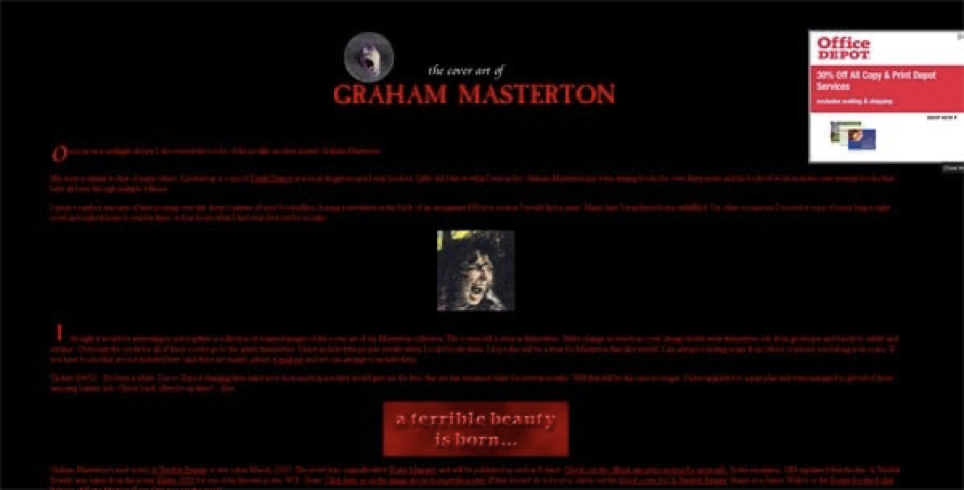
\includegraphics[width=0.8\textwidth]{figures/bad-colours_black.background-1}
    \label{fig:bad-colours_black.background-1}
    \caption{}
\end{figure}


\begin{figure}[H]
    \centering
    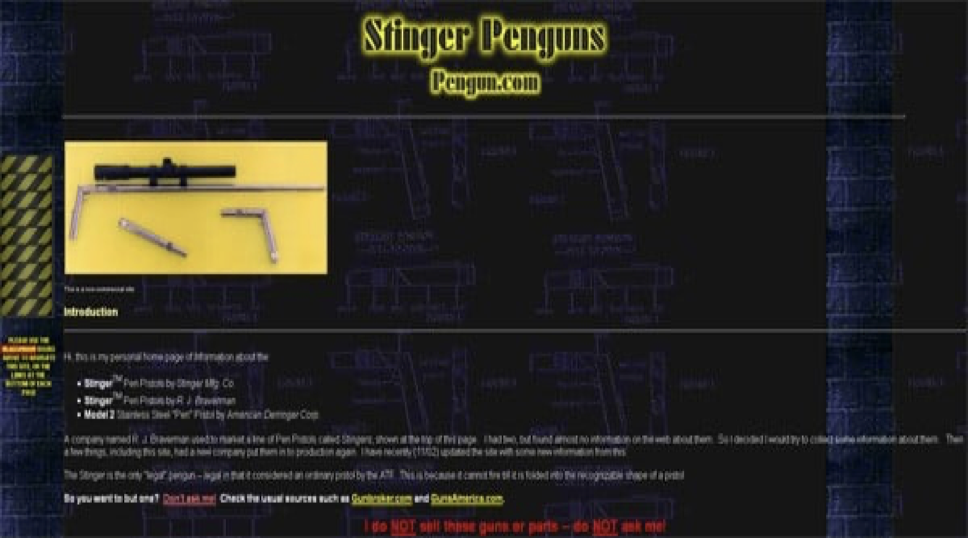
\includegraphics[width=0.8\textwidth]{figures/bad-colours_black.background-2}
    \label{fig:bad-colours_black.background-2}
    \caption{}
\end{figure}



\subsection{Too many colours}
\paragraph{} If in doubt, throw everything against the wall and see what sticks. If choosing the right colours is difficult then why not just use them all? At least then you've got all the good combinations in there amongst the bad ones? It turns out that this approach doesn't work so well from a design perspective.



\begin{figure}[H]
    \centering
    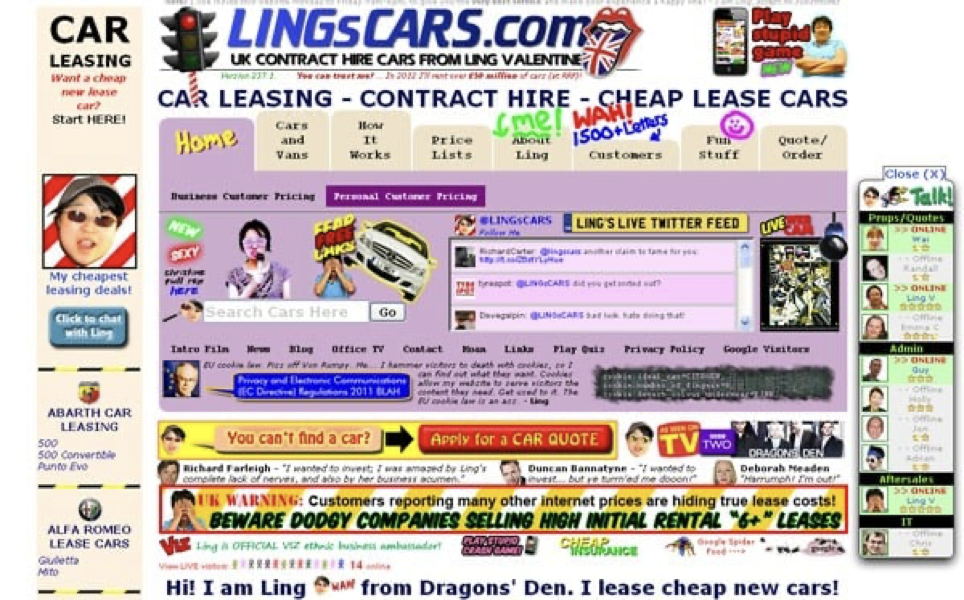
\includegraphics[width=0.8\textwidth]{figures/bad-colours-too-many-colours-1}
    \label{fig:bad-colours-too-many-colours-1}
    \caption{}
\end{figure}


\begin{figure}[H]
    \centering
    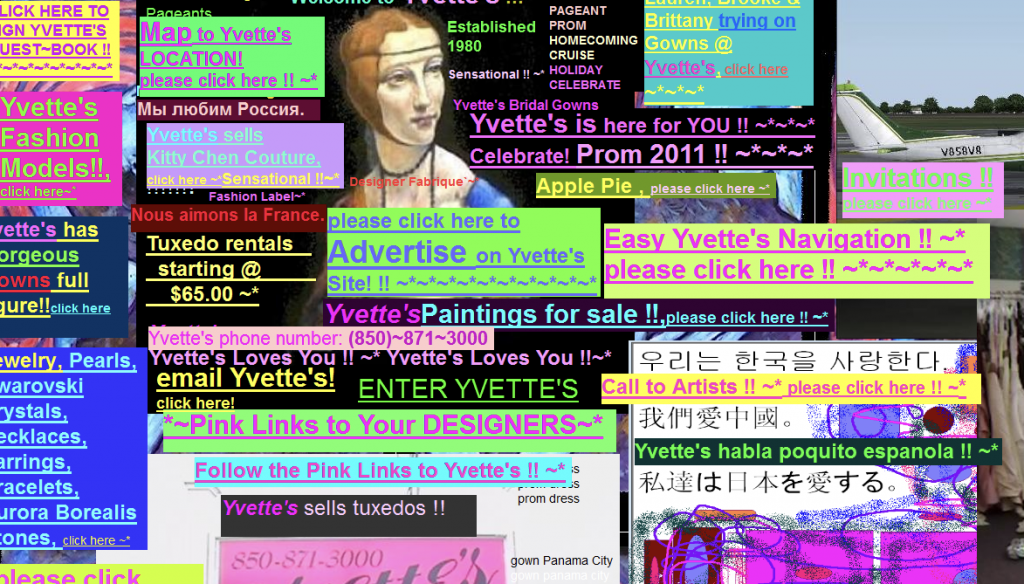
\includegraphics[width=0.8\textwidth]{figures/bad-colours-too-many-colours-2}
    \label{fig:bad-colours-too-many-colours-2}
    \caption{}
\end{figure}


\paragraph{} Note that this example has a number of issues, combining a complex background with the use of a lot of colours. I understand why it has been done, it makes sense to use the colours of the German flag as a starting point for the theme given the subject matter of the site, but this is hard to do effectively.



\begin{figure}[H]
    \centering
    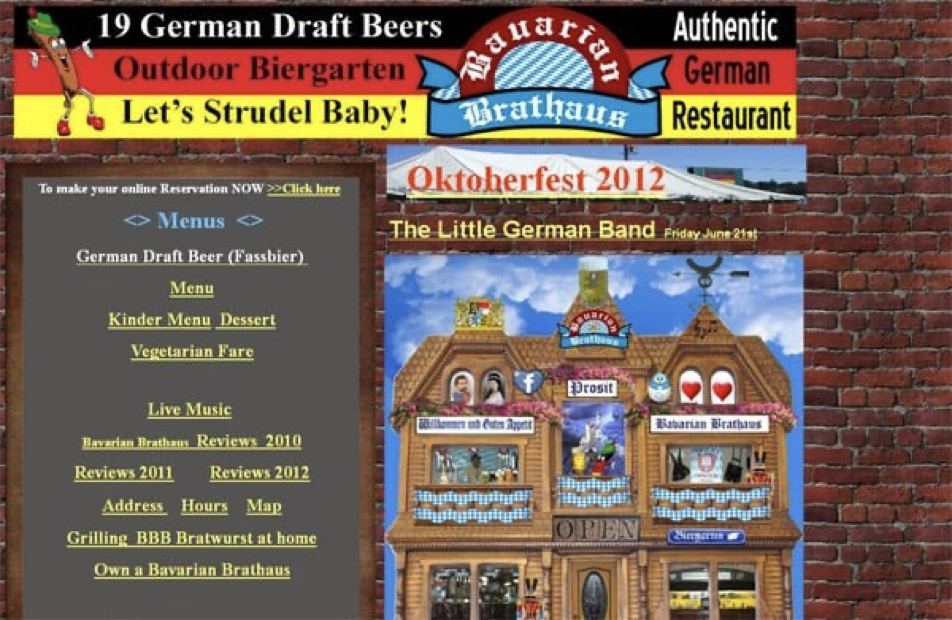
\includegraphics[width=0.8\textwidth]{figures/bad-colours-too-many-colours-3}
    \label{fig:bad-colours-too-many-colours-3}
    \caption{}
\end{figure}





\subsection{Predominant use of blue as background}
\paragraph{} As with black and green, most shades of blue can also make a poor choice of background. This is partly due to issues of insufficient contrast and partly due to the tendency of blue to dominate other colours. We don't want the background to dominate the foreground, hence we don't want a more dominant colour to invert the foreground/background relationship.


\begin{figure}[H]
    \centering
    
\includegraphics[width=0.8\textwidth]{figures/bad-colours_blue-background-1}
    \label{fig:bad-colours_blue-background-1}
    \caption{}
\end{figure}


\begin{figure}[H]
    \centering
    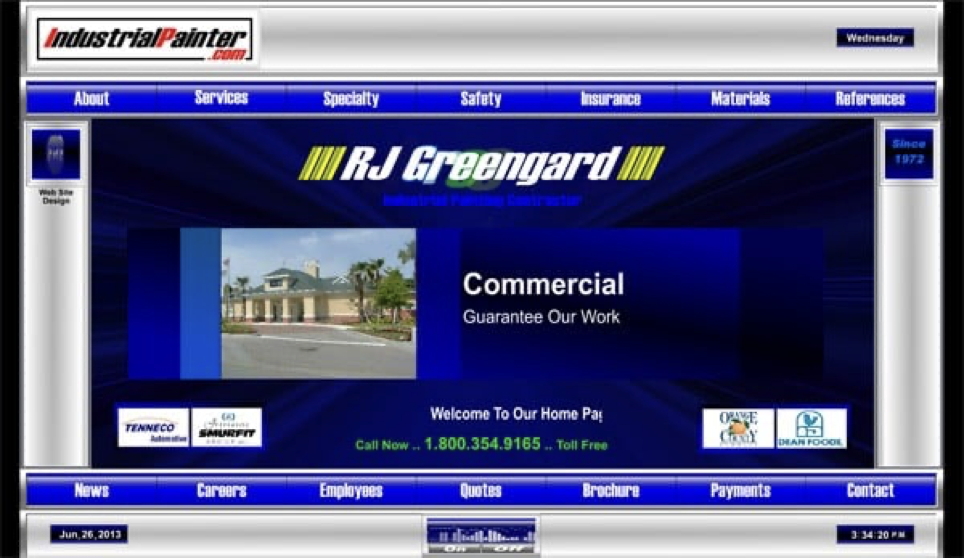
\includegraphics[width=0.8\textwidth]{figures/bad-colours_blue-background-2}
    \label{fig:bad-colours_blue-background-2}
    \caption{}
\end{figure}



\section{Choosing Colours}
\paragraph{} Start thinking about how many colours you need during your design process. This is not a straightforward process. It is not just a case of counting every element and then assigning a different colour for each one. Instead you must consider the relationships between the visual elements of your page. The most important relationship is foreground and background. You must have sufficient contrast between elements in the foreground and elements in the background. If there is too little contrast then your user will have trouble reading the text. However also bear in mind that too much contrast, such as black text on a white background, can be tiring if a lot of reading must be done from the screen. Whilst black on white is generally fine for printed materials, computer screens radiate light rather than reflecting it, and this can alter the visual perception as a result. So a good compromise is often the level of contrast that you might get with off-black text against an off-white background. However, as you've probably already noticed, most sites have a palette of colours with more than two elements for the foreground and background, so consider all of the other elements, perhaps headings, emphasised text, body text, hyperlinks, boxes, semantic blocks, \&c. and decide whether you want them to share colours or have separate colours.
\paragraph{} This process will give you an idea of how many colours you need in you palette but not concerned with what the colours are yet. As noted above, colours can be re-used in multiple places, so aim to minimise the number of colours rather than maximise. A five colour basic palette is very common even for complex sites. Many, if not most, colour schemes are in the range of between 5 and 9 elements with perhaps two elements, with fairly good contrast between them, being dominant in usage over the remainder. It can be worth trying out your colour scheme against your design document, if you've created one, as this can give a good way to rapidly see how all of the elements that make up your site will juxtapose against each other and also lets you easily apply the same colour scheme in different ways.


\section{Palette Selection Tools}
\paragraph{} As many aspects of colour selection are fairly mechanical, a reliable solution, if you don't have an artist's eye, is to use a colour palette selection tool. These palette building tools are designed to use various aspects of colour theory and "complementary colours" to select the elements of your palette for you.

\paragraph{} For example, you select a dominant or base colour for the scheme and the rest of the palette is built around that choice. The tool selects complementary, monochromatic, triad, analogous, compound, or shade based groups of colours for you from the colour wheel on the basis of colour theory. All you must do is decide how big your palette of colours needs to be, but you should have some idea of this already from your mockup activities.

\paragraph{} Once you have your palette, which in practise might just be a list of colour hex numbers, you can then apply it to your design. You should aim to apply the colours from the tool consistently in implementing your design. Don’t deviate and choose a different colour to replace an element of the palette as this can negatively affect all of the colours matching in the rest of the palette. Instead if you need to deviate from the colour palette you've built, then it means that there is probably another iteration of design required to fine tune the elements that make up the site.

\paragraph{} Similarly, if you run out of colours then return to the palette tool and increase the size of the generated palette and reapply all of the adjusted colours to your design. This is why separating out HTML (markup/structure/representation) and CSS (presentation) is a good thing, altering the CSS alters everywhere it is used throughout your site.

\paragraph{} This is a selection of common online palette generation tools:

\begin{itemize}
\item \url{https://coolors.co/}
\item \url{http://www.colourlovers.com/palettes}
\item \url{http://paletton.com/}
\item \url{http://www.color-hex.com/color-palettes/}
\item \url{https://color.adobe.com/create/color-wheel/}
\end{itemize}

\paragraph{} There are others. Find one that you like and which you can use effectively. I've used coolers quite extensively in the past as a simple and easy way to get started and it looks like this:

\begin{figure}[H]
    \centering
    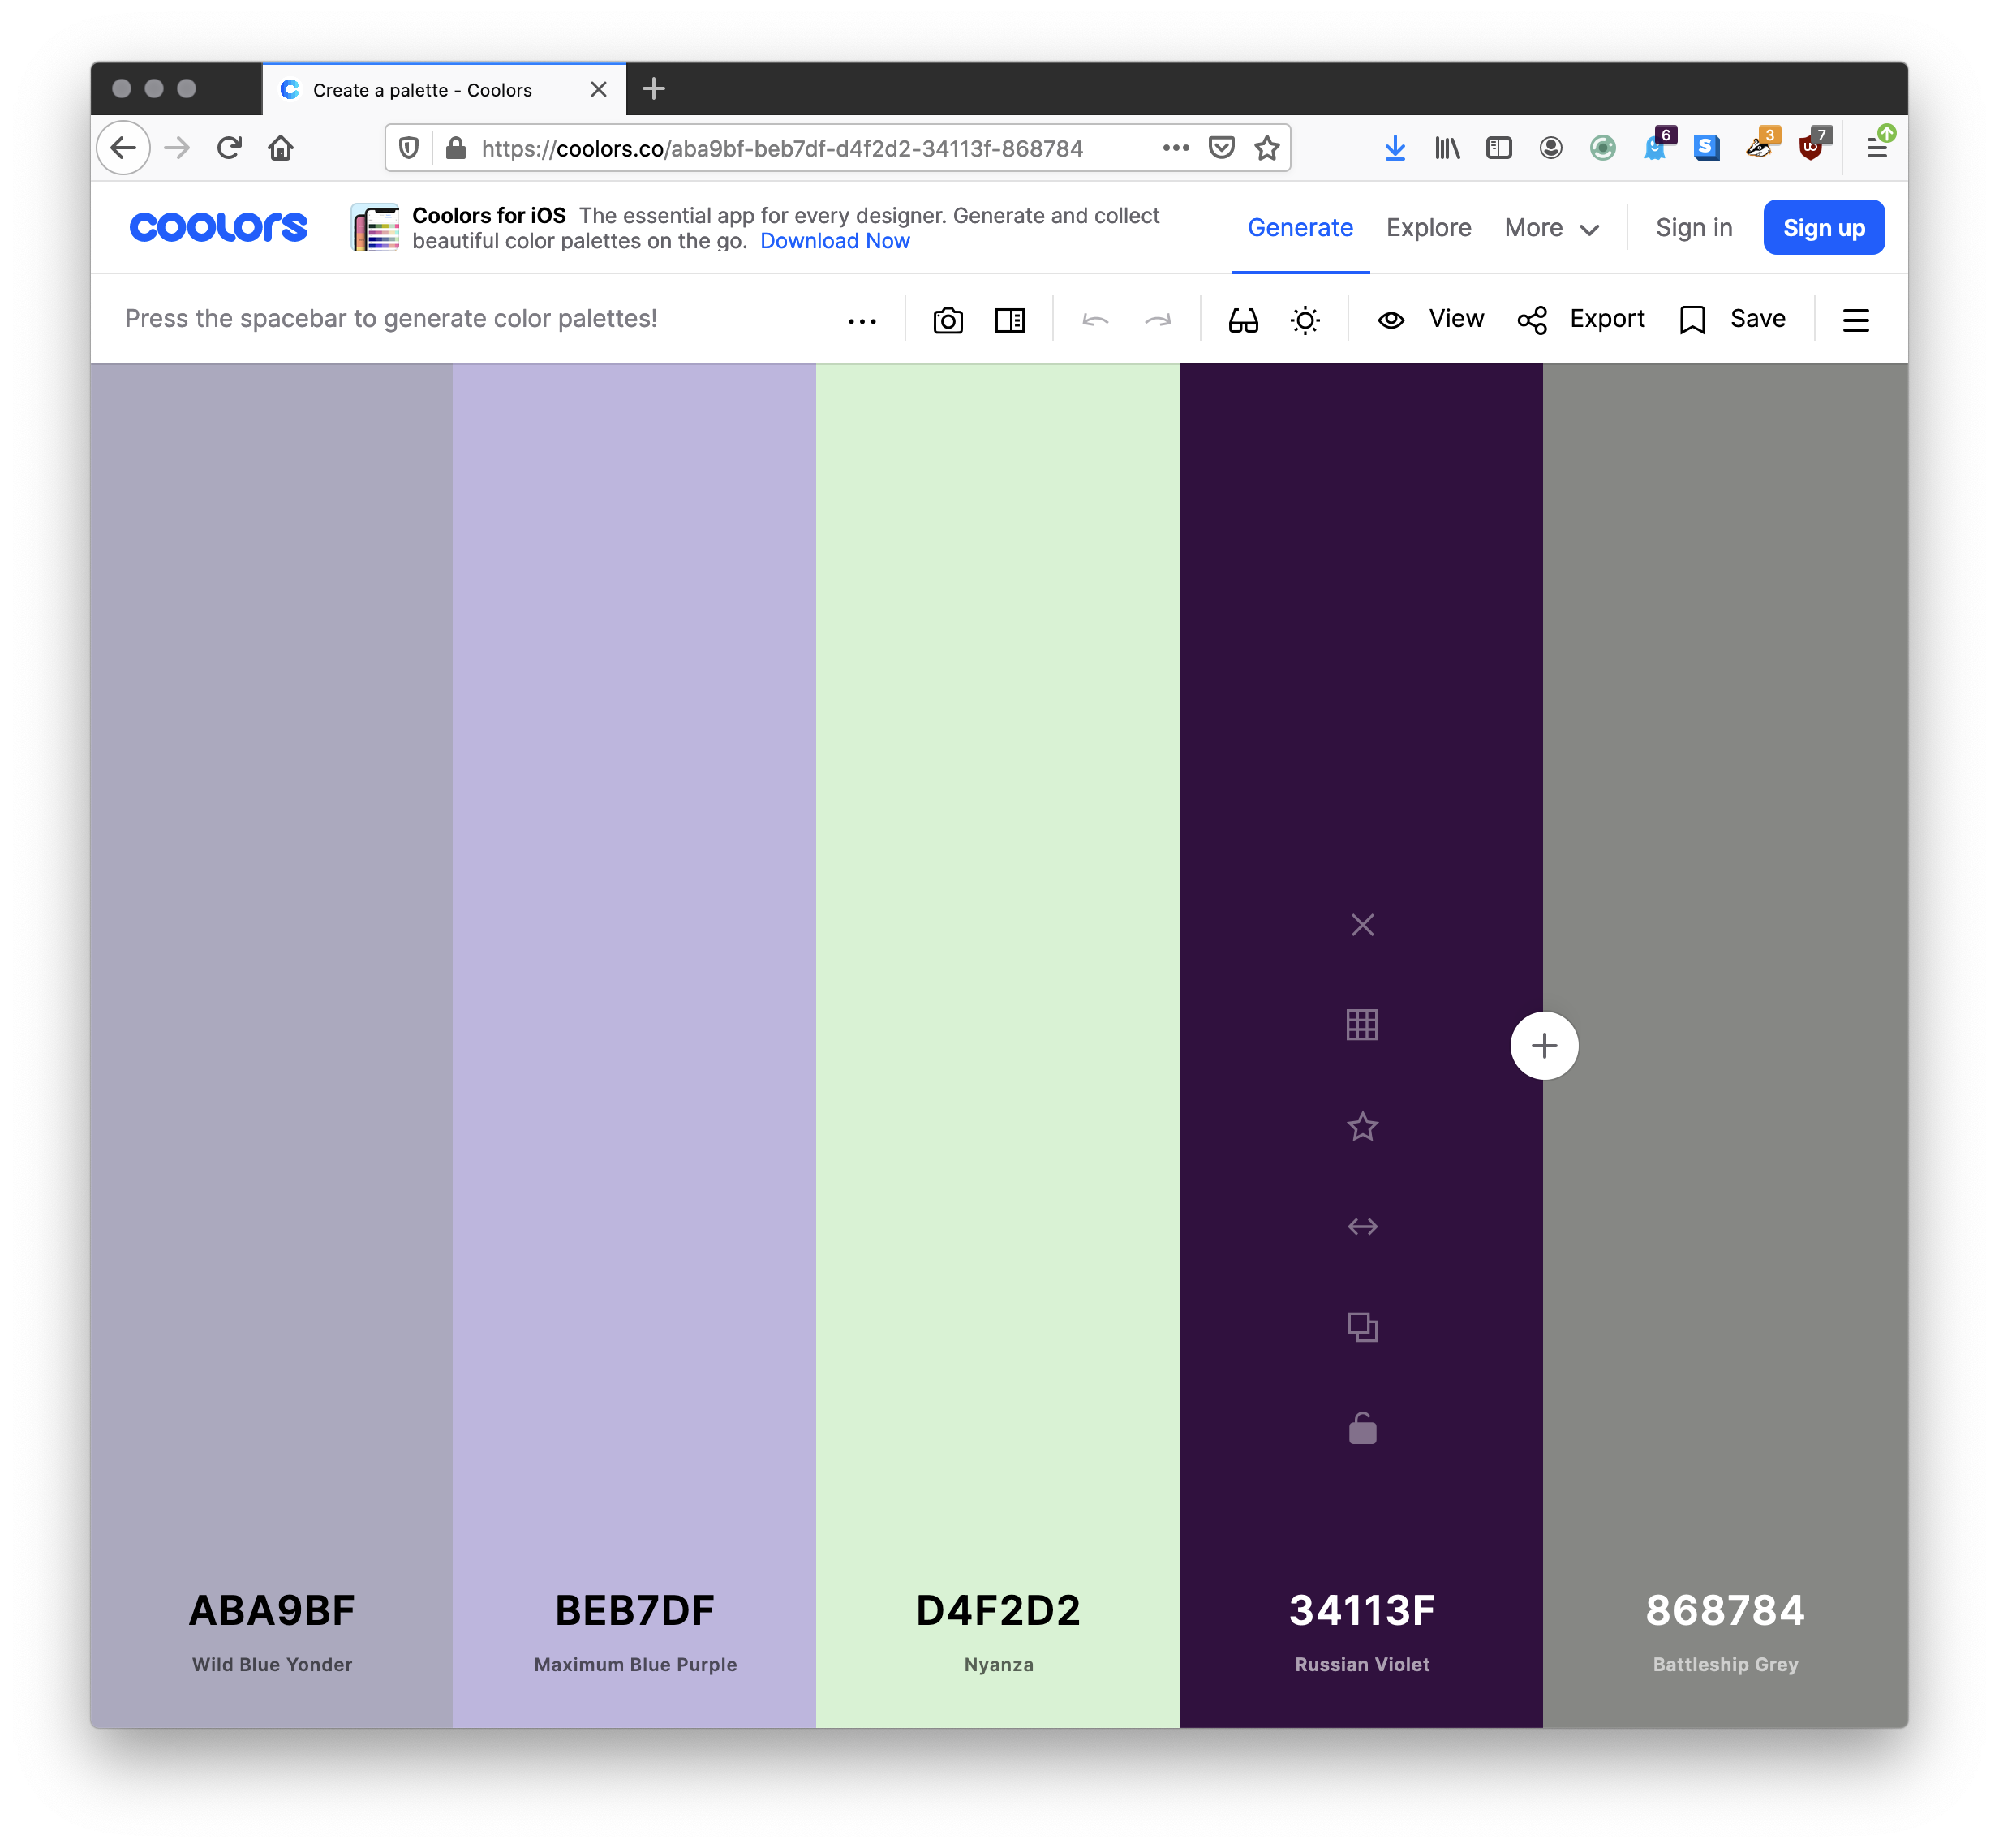
\includegraphics[width=0.8\textwidth]{figures/generated-palette-example}
    \label{fig:generated-palette-example}
    \caption{}
\end{figure}


\paragraph{} You can use the ``+'' icon when hovering over any colour to add additional colours, up to a maximum of 10 using the free version, and can return to any given colour scheme if you use the same URL, so bookmark your favourite schemes, or even better, note the address with its unique ID in your design documentation.



\section{Design Guidelines}
\paragraph{} Once you've been through the design process, creating mockups, and making design decisions about such things as colour-schemes and visual presentation, you might ask yourself what the result should be. For some the set of mockups and designs is sufficient and you can move straight to implementation.
\paragraph{} However if your site is going to have a longer life, or will be further developed by other people, or is meant to integrate into a wider organisation where there might be print, video, and other artefacts in addition to the website, for example, where there is a wider, perhaps corporate, brand identify beyond just the site, then it can be useful to document the designs and decisions somehow.
\paragraph{} One approach to this documentation process is to develop design guidelines. These document design, interaction, and user experience decisions so that new additions and modifications are consistent. Design guidelines are a cohesive description of the look and feel of your site that describes every element. This can be used to make sure you are consistent in applying your design and to make sure that others are consistent because they have a reference to which they can refer. Note that just a few out-of-design ``additions'' can turn a well designed site into something of a dogs dinner. By documenting your design you can extend the life of your project by helping to make it much more maintainable and enabling every design aspect to be referenced.
\paragraph{} Design guidelines can be very extensive and complicated, they can become as complex as a language for detailing every aspect of your site, or be as simple as a single HTML page that demonstrates all the CSS and presentational aspects you’ve used. We'll look at both approaches now.

\section{Design Documents}
\paragraph{} These are also known as ``Pattern Portfolios'' or ``Style Guides''. On the simplest level this can be a single deliverable, comprising a single HTML page which contains an example of every element, style, and component for your site. This way you can see how every aspect of your design looks in context with every other component all in one place. Developers can then use this as a reference when implementing individual pages within the site. As the design document is an HTML page and uses the live CSS for the site, then any changes to the design document are reflected throughout the implementation. In addition, because the HTML and CSS are both text, they can be committed to your source-code repository (perhaps in a  folder named /design) and the version history can be tracked. 
\paragraph{} Note that design documents can be more complex than a single page, using as many pages as necessary to completely document the design. This should be driven by the need to balance keeping the document as small and easy to use as possible, whilst also adequately documenting the design.
\paragraph{} Some people make their design documents public as part of their live site. Here are two examples of that

\begin{itemize}
	\item https://paulrobertlloyd.com/styleguide/
	\item http://oli.jp/2011/style-guide/
\end{itemize}


\subsection{Example Design Document}

\paragraph{} Here we have a visual example of a design document.

\begin{figure}[H]
    \centering
    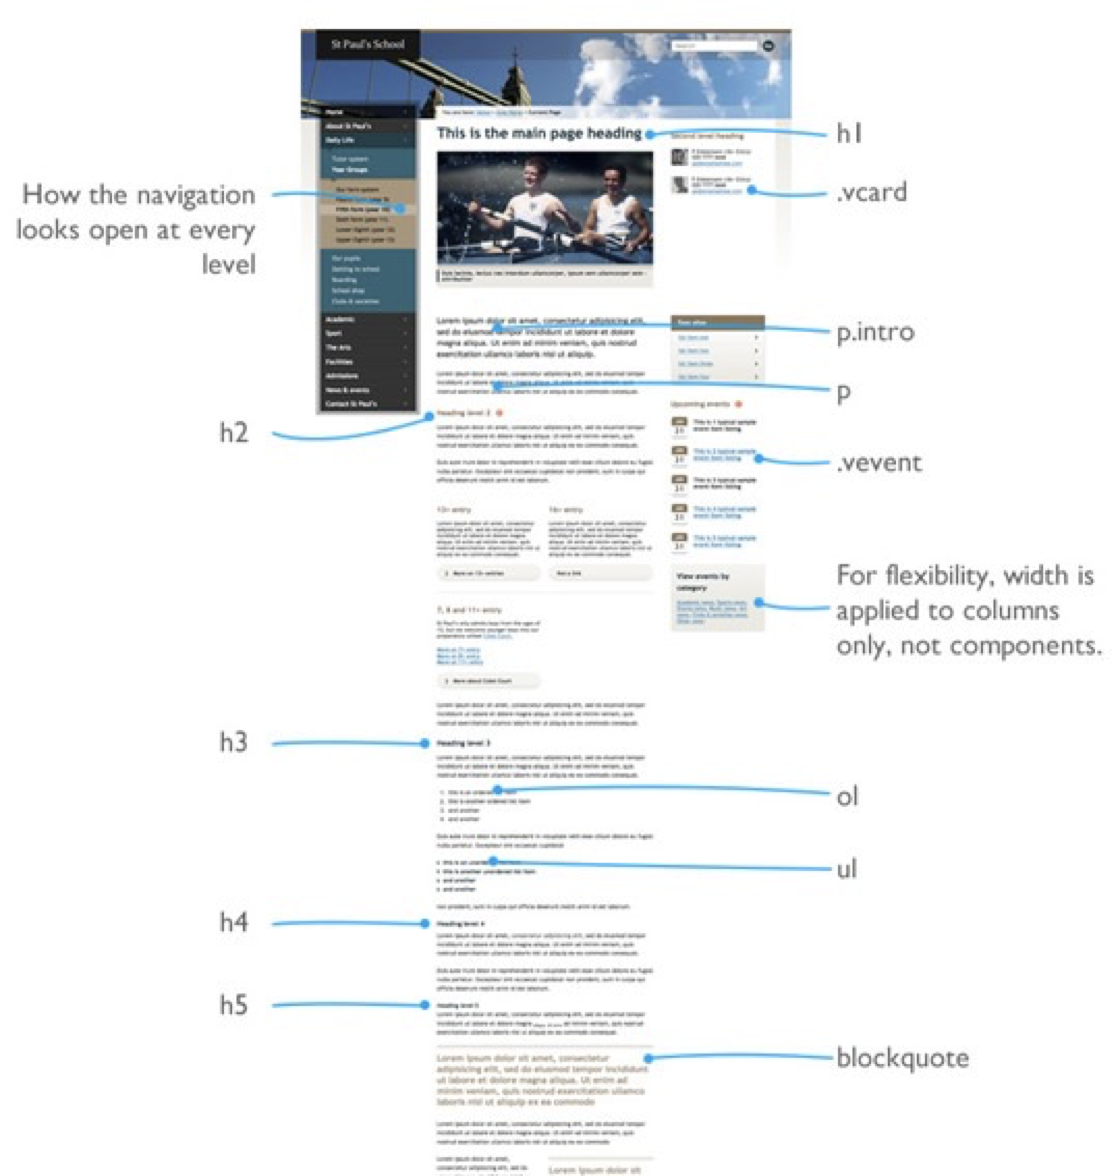
\includegraphics[width=0.8\textwidth]{figures/design-document-example}
    \label{fig:design-document-example}
    \caption{}
\end{figure}


\section{Design Guidelines In the Wild}
\paragraph{} Design guidelines beyond the design document are used by many organisations to design and document:

\begin{itemize}
	\item Websites
	\item Mobile apps
	\item Paper comms (posters, flyers, leaflets) — remember that paper is still very relevant for public communication
\end{itemize}

\paragraph{} Remember that communications in larger organisations aren’t just for the Web but will often be multi-modal, hence the design guidelines might cover more than just the Web. The results can be large, diverse, and particular to the needs of the specific organisation. The best way to get to grips with these is to explore some examples.

\subsection{TfL Design Standards}
\paragraph{} TfL (Transport for London) publishes a corporate design standard\footnote{\url{https://tfl.gov.uk/info-for/suppliers-and-contractors/design-standards
}} to ensure that all communications maintain their design ideals
\paragraph{} ``This guide is designed to help us work as one brand, and to make it easier to produce high quality communications, experiences and propositions both internally and externally.''

\subsection{NHS Brand Guidelines}
\paragraph{} The NHS Brand Guidelines\footnote{\url{https://www.england.nhs.uk/nhsidentity/}} have a slightly different focus (England Wide) and covering local GP practices as well as hospitals and `corporate' communication. Aims to enable local doctors to develop materials, e.g. information leaflets, that are in keeping with wider NHS corporate branding standards
\paragraph{} There is an additional element of trust here. There is lots of health communication that is quackery at best and outright dangerous at worst. Important to establish provenance.

\subsection{BBC GEL}
\paragraph{} A GEL is a Global Experience Language. Global refers to the whole experience and the reach of the resulting artefact. The BBC use their own GEL\footnote{\url{http://www.bbc.co.uk/gel}} to ensure that all sites under the BBC brand are coherent

\subsection{Edinburgh University GEL}
Edinburgh university developed its own GEL\footnote{\url{http://gel.ed.ac.uk/}} to support best practices in the promotion of their University brand.


\section{Some Design Hacks for Coders}
\paragraph{} The following is an annotated list of rough design hacks and rules of thumb that I've gathered and generally adhered to over the years. They aren't hard and fast rules, but are instead a useful starting place. Apply them as works for the context in which you're working.

\begin{itemize}
\item Use palette selection tools to generate a decent set of colours then use those colours carefully and deliberately by applying them to your design. This presupposes that you have an idea for a design.
\item Sketch out or else mock-up a design. This will likely be a living document and change greatly, but enables you to start working out how your site content will come together. Even if you don't have any content yet, you will probably have some idea of the kind of content that you will have in the future.
\item Mock-up your layout using greeked text if you don't yet have any written content. In the meantime the greeked mock-up will enable you to still make some progress.
\item If you do have content but you don't have any ideas for a design then remember that form can follow content. So why not try starting with an HTML only version of your site and content. This will give you a good skeleton to work with as your design matures. By doing this you might better understand the structure of your content which might make the design aspect easier.
\item Don't try to fill the page. Your content will develop over time. Your pages might look fairly empty initially. That is fine.
\item Make good use of whitespace. This is a corollary to not filling the page. Any content you do have should not be too cramped. Try to make good use of the CSS box model and make sure that the elements of your page have room to breathe, for example, using margins effectively around text can make for a much better reading experience. Think about when you create a written document, you leave white space all around the edge, even though it may seem wasteful, mainly because this makes it easier to read.
\item Don’t use too much whitespace. Another corollary to not filling the page and making good use of whitespace is to not go overboard. We still want good information density in our interface so that our user doesn't have to scroll too much. Our eyes will often skip around the page when reading and take in much more than we expect. The more that we have on screen, the more we can take advantage of this. This also means thinking about your content, if there is data that users might want to compare, then designing so that all of that information is close together and can be seen together on screen is not a bad idea.
\item Use less furniture (rules, boxes, dots, outlines) around your page elements. Sometimes we are tempted to draw a box around things to set them off against other elements, or to delineate boundaries, but this is more visual clutter and can detract from the clarity of your message. It can be worth using less visible furniture sometimes to delineate your data, or else making appropriate use of whitespace to isolate individual elements from each other.
\item Spacing and alignment are hugely important especially when comparing data. For example, when skimming over data it is easier when things are aligned vertically, particularly for numeric data but also for regular reading of text. As a result you should rarely need to center text other than perhaps in headlines or to isolate something special, but most prose should be left justified to enable your reader to skim over your paragraphs, allowing their eye to jump easily down the page. As normal text fonts have variable sizes between sigils it is worth selecting a monospaced font if you need to align digits in numeric data but bear in mind that such fonts are problematic for regular reading of non-numeric data. Similarly, if you are dealing with currency, aligning decimal points  can help your reader. Narrow line-heights between rows of data can keep data close together. But note that your data should still be cleanly separated. This might involve some trial and error, but the goal is to get a good density of information viewable at once without cluttering things and reducing comprehension.
\item You can also attempt to reduce the volume of data when it is presented visually. The visual presentation of your data can be different to the internal, stored representation. This process of reducing volume should be governed by what functionality you are trying to provide. For example, why have both first and last names in separate columns when they can be combined into a single “name” when displayed? Similarly, why have separate columns or rows for each of Town, County, and Postcode when they could be joined and displayed as a single "address" datapoint. Note though, that if the user has to interact with these things as separate data then you might opt not to combine them. As a result, this is driven by the needs of the site, the users, the data, and the design. It's worth removing redundant data and anything else that the user doesn’t need to see from your page. As a rule, it is better for privacy preservation, and any associated security aspects if you consider that you can't lose or accidentally disclose user data if you don't possess it. So, generally, don't collect data that you know, or are pretty sure, that you don't need.
\item Get feedback on your designs. Ask potential users and show them what you're doing and solicit their feedback. Note though that they can be wrong, they can have an idea of what they think they want and can be vocal about it, until you show them your novel new design that they hadn't ever considered. If you do engage with your users then watch them perform their tasks and use that as inspiration for your design, but don’t slavishly reimplement real-world procedures if there is a better way. Remember that users who are doing things in the real world might have some great ideas about how to streamline the process.
\item Perhaps most important, remember that you’ll never make the perfect UI for all people, so why not let your user export the data from your site using a common format, for example, using a Comma Separated Values (CSV) file, JSON, or XML. Your user can then use an appropriate tool to manipulate the data in the ways that they need to. For example, tabular data, that is, data arranged in row and columns, can be easily exported as a CSV file and then loaded into any spreadsheet applications or manipulated using a scripting language. This is much more flexible than trying to account for all the ways that a user might need to use data within your web interface.
\item If in doubt, and all else fails, use an existing CSS design solution, such as bootstrap, as a shortcut to a pleasing prototype.
\end{itemize}


\section{Summary}
\paragraph{} In this chapter we've considered the importance of design with respect to some real world problems and have considered the potential consequences of poor design. We've also explored some aspects of prototyping our sites, mocking up content, and selecting colour. We've then finished by considering some ``Design Hacks for Coders'', a collection of heuristics for guiding you towards creating better designs.


\chapter{Core JS}
\label{core-js}
\paragraph{} 



\chapter{Client-Side JS: Browser APIs}
\label{browser-apis}
\paragraph{} JavaScript is how we add dynamism to our web pages mostly through a set of global JS objects which provide access to the client environment. So now we have a working knowledge of Javascript, we'll start to look at how it can be used to manipulate the HTML that makes up our webpages, as well as to interact with the browser. If we think of the browser as the host environment that defines the space in which our Javascript functions run, then it is useful to explore what features of the environment are made available to us through the Browser's Application Programming Interfaces (Browser’s APIs).


\section{JS \& HTML}
\paragraph{} In the last unit we considered how JS practically interacts with other web technologies. In particular:

\begin{itemize}
\item JS isn’t self-hosted within the browser. That is we can't just retrieve a JS file directly from a web address and run it. The JS has to be hosted within a page. A minimal host document is required to cause the browser to then retrieve our JS. Once retrieved the JS is then loaded and executed by the browser's JS engine.
\item JS can be:
    \begin{itemize}
    \item added inline with HTML elements, 
    \item spread throughout our document, or 
    \item added as a block collected into a single place within a document, or as an external/linked file(s)
    \end{itemize}
\end{itemize}

\paragraph{} Note that our examples from the last unit were all run in the browser web console. Whilst strictly speaking this means we can run JS in the browser, it actually gives us a fairly rich environment for executing JS, learning the language, and experimenting, but it isn't generally how we would distribute our JS code to end-users

\paragraph{} We’ll investigate this a little more and use it as a motivating framework for exploring interactions between HTML and JS. In the last unit we briefly surveyed three methods by which JS can be integrated with HTML. Let's recap those now.


\section{Recap: A Simple Inline JS Example}
\paragraph{} In this example we have our JS entirely encapsulated within the onclick function of an HTML button element.

\begin{lstlisting}
<!DOCTYPE html>
<html>
  <head>
    <title>Example</title>
  </head>
  <body>
      <button onclick="var textNode = document.createTextNode(‘Napier!');
 			document.body.appendChild(textNode);">Hello</button>
  </body>
</html>
\end{lstlisting}

\paragraph{} This means that our JS is localised entirely to the specific button element that it is attached to and can't be reused elsewhere, for example, if we have similar code attached to another button. This means that you need to repeat code across your pages, as well as mix JS amongst your HTML. Generally this is a bit of a "code smell" and, whilst useful for quickly trying out some code, is not an ideal solution.


\section{Recap: A Simple JS Script Block Example}
\paragraph{} This version moves our JS into its own script block. Note that it doesn't do anything more than our last, inline, version. In fact it needs a little bit more code to achieve the same effect. This is mainly because the inline version is immediately attached to its HTML element and the context in which it runs. Now we've separated our JS from the HTML element it affects, we have to add additional code to get a 'handle' on the original HTML element. In this case we've achieved our aims by adding an ID to the button and then using getElementById to create the link between our JS and the button element.

\begin{lstlisting}
<!DOCTYPE html>
<html>
  <head>
    <title>Example</title>
  </head>
  <body>
    <button id="hello_btn">Hello</button>
    <script>
        document.getElementById('hello_btn').onclick = function() {
           var text_node = document.createTextNode('Napier!');
            document.body.appendChild(text_node);   
        };
    </script>
  </body>
</html>
\end{lstlisting}

\paragraph{} Overall, the JS is now reasonably separated from the HTML elements within the page which means that functions can be more easily organised and reused in multiple places. Whilst the JS is still hosted within the parent HTML document it is encapsulated within a pair of script tags. This actually makes it much easier to move to the next integration method\dots


\section{Recap: A Simple JS Eternal Script Example}
\paragraph{} In this example our JS is now entirely stored within a separate file. First our index.html file:

\begin{lstlisting}
<!DOCTYPE html>
<html>
  <head>
    <title>Example</title>
  </head>
  <body>
    <button id="hello_btn">Hello</button>
    <script src="tmp.js"></script>
  </body>
</html>
\end{lstlisting}

\paragraph{} and then our index.js file:

\begin{lstlisting}
document.getElementById('hello_btn').onclick = function() {
    var text_node = document.createTextNode('Napier!');
        document.body.appendChild(text_node);   
};
\end{lstlisting}

\paragraph{} Notice that we still have a script tag in the HTML file, but it now just points to a web address where the JS is located and can be retrieved from. Again, the only link between the HTML element, our button, and the JS that is executed when the button is pressed is the button's ID.
\paragraph{} The pattern found in this example is probably the most standard framework for relating JS and HTML, keeping a useful separation of concerns that can lead to better manageability and increased reusability of code.



\section{A Slightly More Complex Example}
\paragraph{} The last example was fairly static though, it didn't do much other than wait for user input. The following example goes a little further. As well as giving us a button that, when clicked, adds text to the page, we're also actually building the page itself. Look at the body of our HTML file. It doesn't actually contain any HTML elements, so where is our interface coming from? It turns out that we're building it entirely through JS code! This is a really powerful opportunity that JS provides us for dynamically changing the pages that our users see.

\begin{lstlisting}
<!DOCTYPE html>
<html>
  <head>
    <script src="tmp.js"></script>
  </head>
  <body>
  </body>
</html>
\end{lstlisting}

\paragraph{} and our index.js file:

\begin{lstlisting}
function init() {
    document.title = "Hello Napier Example"

    var button = document.createElement("button");
    button.innerHTML = "Hello";
    button.id = "hello_btn";
    var body = document.getElementsByTagName("body")[0];
    body.appendChild(button);

    document.getElementById('hello_btn').onclick = function() {
        var text_node = document.createTextNode('Napier!');
            document.body.appendChild(text_node);   
    };
};
window.onload=init;
\end{lstlisting}


\section{The JS-HTML Relationship}
\paragraph{} On a practical level the JS-HTML relationship, where an HTML document references some JS that then runs, is a simplified way of looking at things. It is actually not merely the case that the browser retrieves an HTML document, which in turn references some JS, which then just runs.
\paragraph{} The reality is a little more complex. You can get away with the above understanding but you’ll miss a lot of powerful functionality if you don’t consider the wider context of the DOM (the Document Object Model) and the browser environment. A lot of rich possibilities are created by the set of APIs that the DOM and browser environment provide.
\paragraph{} To understand this relationship, and to start seeing some of the possibilities that are provided, we’re going to primarily consider the following in this unit:

\begin{itemize}
\item The Window Object
\item The Document Object
\end{itemize}



\section{The Window Object Hierarchy}
\paragraph{} The Window object is the root of a tree of browser and web page related objects along with their associated APIs. One of the children of the Window object is the document object, which gives us access to the DOM. All of the other children give us access to the wider infrastructure that we can manipulate, all related to the browser window. Not only are we able to interact with the parsed HTML document (our current page) but also with a wide range of additional related aspects of the browser. 
\paragraph{} More specifically these are additional objects that JS can access and hence we can write JS code to manipulate them within the boundaries provided by their respective APIs.
\paragraph{} Note that there are browser differences which mean that some objects are available on some platforms/versions and not on others. For the most part this is not an issue, but you should be aware of the possibility. The diagram gives you an idea of the range of objects that are accessible to our JS code.

\begin{figure}[H]
\centering
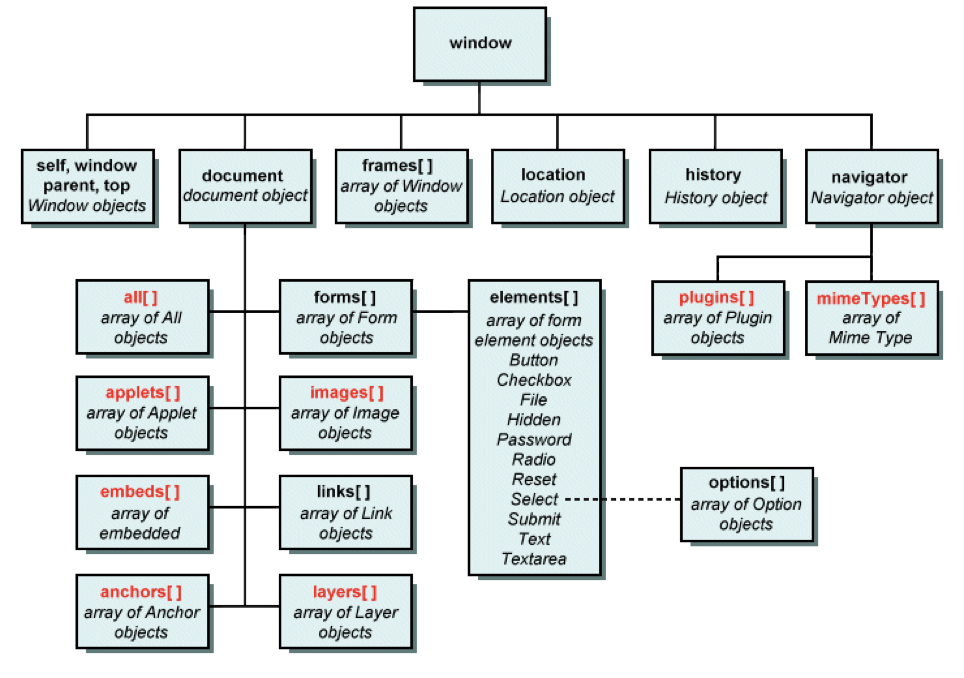
\includegraphics[width=0.8\textwidth]{figures/window-object-hierarchy}
\label{fig:window-object-hierarchy}
\caption{}
\end{figure}



\section{Global Objects}
\paragraph{} First an aside about global objects and scope. Generally our JS code is either associated with a Window and hence has a Window object associated with it, or else it runs in a separate background task within the browser. We'll not specifically cover background tasks here, they are a way to run your code "in the background" so that it doesn't interfere with the responsiveness of the current tab. This can be very useful for more involved JS applications so if you want to know more then it is worth researching the term "webworkers" if you do want to run bits of code independently in the background.
\paragraph{} The window object is a global object. This means that it is always in scope or has “global scope”. Any JS variables that you create outside a function also have global scope. Additionally any JS functions that you create outside an object have global scope. What does this mean? That we can always access the Window object, from any part of our code, and that any global variables, or functions that we create are also accessible via the Window object. If we define a global JS variable or function then we can always access it via the window object as a property of the global object.
\paragraph{} Let's look at an example of that:

\begin{lstlisting}
var daka = “more daka”;
daka === window.daka;
// This will evaluate to true if the daka variable is available via the window object

function hi() {console.log(“hi”);}
window.hi === hi;
// Will evaluate to true for the same reasons as above
\end{lstlisting}

\paragraph{} All we've done in the example is to create a variable and a function with global scope, then demonstrated that they are accessible through the Window object.


\section{The Window Object}
\paragraph{} The Window object represents an open browser window, or a tab within a window, for browsers which support tabs. The Window object contains a document object, representing the DOM, the parsed and instantiated set of objects that the browser creates to represent the HTML element described in the source HTML document.
\paragraph{} So our HTML page, as identified by the Web address we've navigated to, is a part of the Window object via the document/DOM child object, but it also gives access to much more.
\paragraph{} For example, a single window could use HTML frames to display multiple HTML pages in the same window, so there is also support for listing, retrieving, and interacting with frames and hence the pages they contain, using the window.frames property.
\paragraph{} Similarly we can find out information about the browser that our page is loaded into via the window.navigator property. This can be used to retrieve, for example, the name of the browser application and its version.
\paragraph{} We can also interact with the history of the current window. By history we mean the list of pages that have been navigated since the current window/tab was opened. Each time you successfully navigate a hypertext link the new page is displayed and the last page is added to the history list. We can find out how long the list of previous pages is and we can use JS to navigate backwards and forward sequentially or to jump backwards and forward between pages. We can also interact with the location (URL/address) of the current page using the window.location property.


\section{The Console Object because ``There will be bugs''}
\paragraph{} The console object provides a really useful set of functions for debugging activities. When you write code, such as JS, you will create bugs. As your code becomes more elaborate, then you are more likely to accidentally introduce bugs. Whilst you will get better at noticing bugs related to syntax, for example, mis-spelling a keyword you will eventually start to create much more subtle bugs, the kind that don't cause a catastrophic crash but are more subtle and corrupt your data or give rise to incorrect results. These bugs are much more difficult to solve. In addition to using the debugging tools that are amongst most  modern desktop browser's suite of developer tools, you can also use the Console object from within your JS code to create log messages of information from within your program. These log messages are displayed in the browser console, and can also be searched and filtered using the browser console tools.
\paragraph{} The console logging functions include console.log, console.info, console.warn, and console.error and can be used to segregate output that is merely informational from output that is important and giving details about errors. You as a developer must decide how important the output is and decide which style of console logging to use for each message that you want to log.
\paragraph{} Logging works by passing a message, a string, to the function, e.g.

\begin{lstlisting}
console.log("Hello Napier");
\end{lstlisting}

\paragraph{} You can also pass CSS styles to logging functions, e.g.

\begin{lstlisting}
console.log("%c hello", "background: #222; color: #bada55");
\end{lstlisting}

\paragraph{} This can make the console much more easy to navigate so that you can find debug information when needed.

\paragraph{} The console also provides access to several other useful debug features that are useful when developing and evaluating our code. These include timing functions, counting and grouping functions, as well as standard debug features like assert() and trace(). We'll look at examples of each over the next few sub-sections.



\subsection{Console Timer Example}
\paragraph{} Sometimes we want to know when something happened, or how long something took to complete, so we use the console.time function to find out. In the following code we create a timer instance, ``t1'' then send log messages to that timer instance before finally ending the timer when we're done. Each call to timelog and timeEnd causes the elapsed time to be displayed in the console.

\begin{lstlisting}
console.time('t1');
console.timeLog('t1', 'starting engines...');
console.timeLog('t1', 'in ur code, doing your things...');
console.timeLog('t1', "work complete, shutting down...");
console.timeEnd('t1');
\end{lstlisting}



\subsection{Console Count() Example}
\paragraph{} Rather than how long something took, sometimes we just want to know how many times something occurred. This ability is what the count function gives us. In the following example we are using the count function to count how many times the greet function is called.

\begin{lstlisting}
let user = "";

function greet() {
  console.count();
  return "hi " + user;
}

user = "bob";
console.log(greet());
user = "alice";
console.log(greet());
console.log(greet());
\end{lstlisting}

\paragraph{} We can also give our counter a label, e.g."alice" so that it can be distinguished from the "default" counter like so:

\begin{lstlisting}
console.count("alice");
\end{lstlisting}



\subsection{Console Group() Example}
\paragraph{} Because our JS programs might become quite large and complex, it can be useful to group and organise our log messages. The console.group function enables us to do this. The console.group function hierarchically groups debug and log output together to make it easier to navigate in the console. Let's look at an example:

\begin{lstlisting}
console.log("This is the outer level");
console.group();
console.log("Level 2");
console.group();
console.log("Level 3");
console.warn("More of level 3");
console.groupEnd();
console.log("Back to level 2");
console.groupEnd();
console.log("Back to the outer level");
\end{lstlisting}

\paragraph{} Running this code in the browser console will give output similar to this:

\begin{figure}[H]
\centering
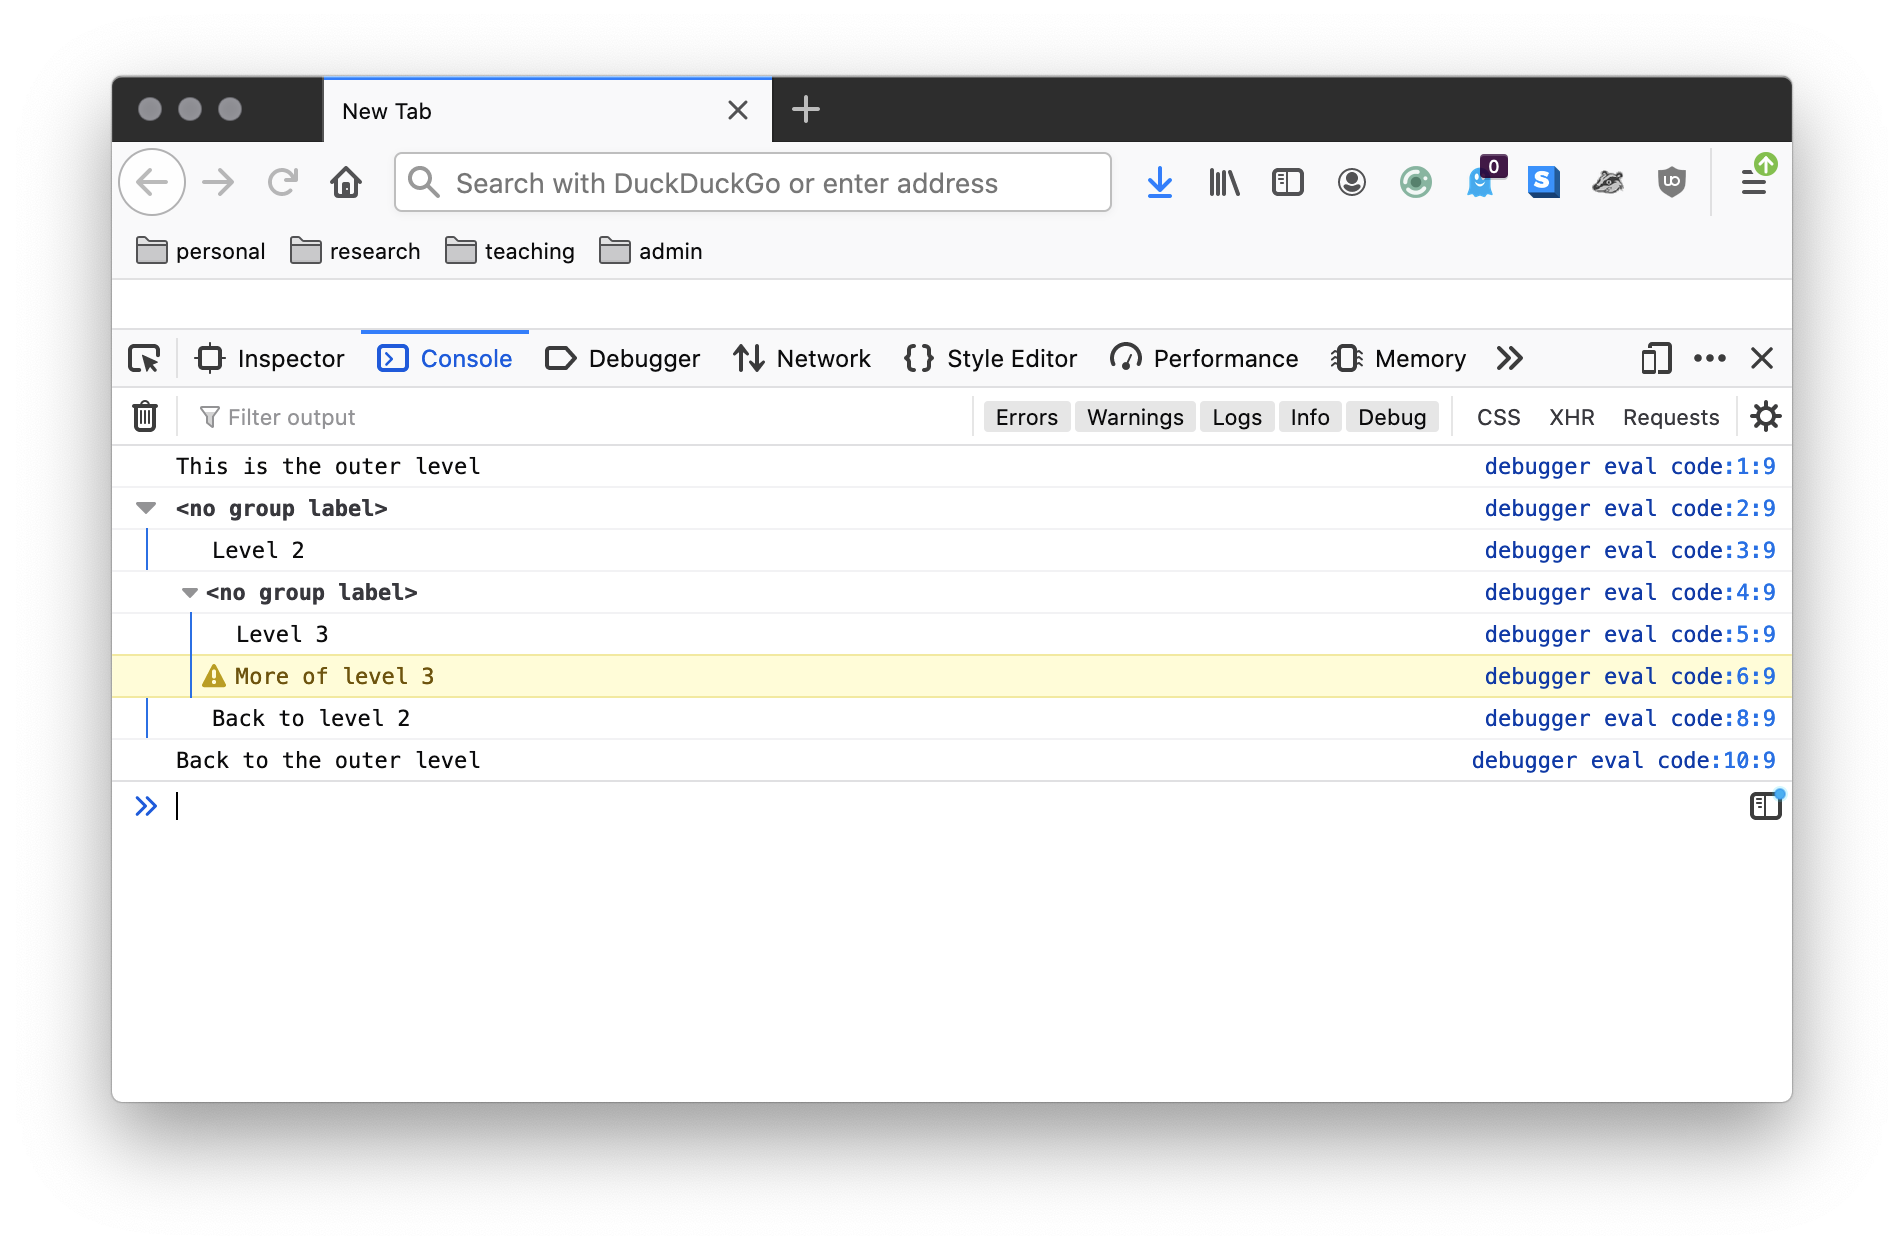
\includegraphics[width=0.8\textwidth]{figures/console-group}
\label{fig:console-group}
\caption{}
\end{figure}



\subsection{Console Assert Example}
\paragraph{} Assertions are used in many programming languages as a way to verify that our expectations about the way that a piece of code works actually match the reality of how it works. The basic idea is that we make an assertion, i.e. the value of variable x at this point in the program is y, and then the actual values of x and y are compared to each other and the assertion is true if they match and false otherwise. Let's look at a small example:

\begin{lstlisting}
const errorMsg = 'the # is not even';
for (let number = 2; number <= 5; number += 1) {
    console.log('the # is ' + number);
    console.assert(number % 2 === 0, {number: number, errorMsg: errorMsg});
}
\end{lstlisting}

\paragraph{} Running this code in the browser console will give output similar to this:

\begin{figure}[H]
\centering
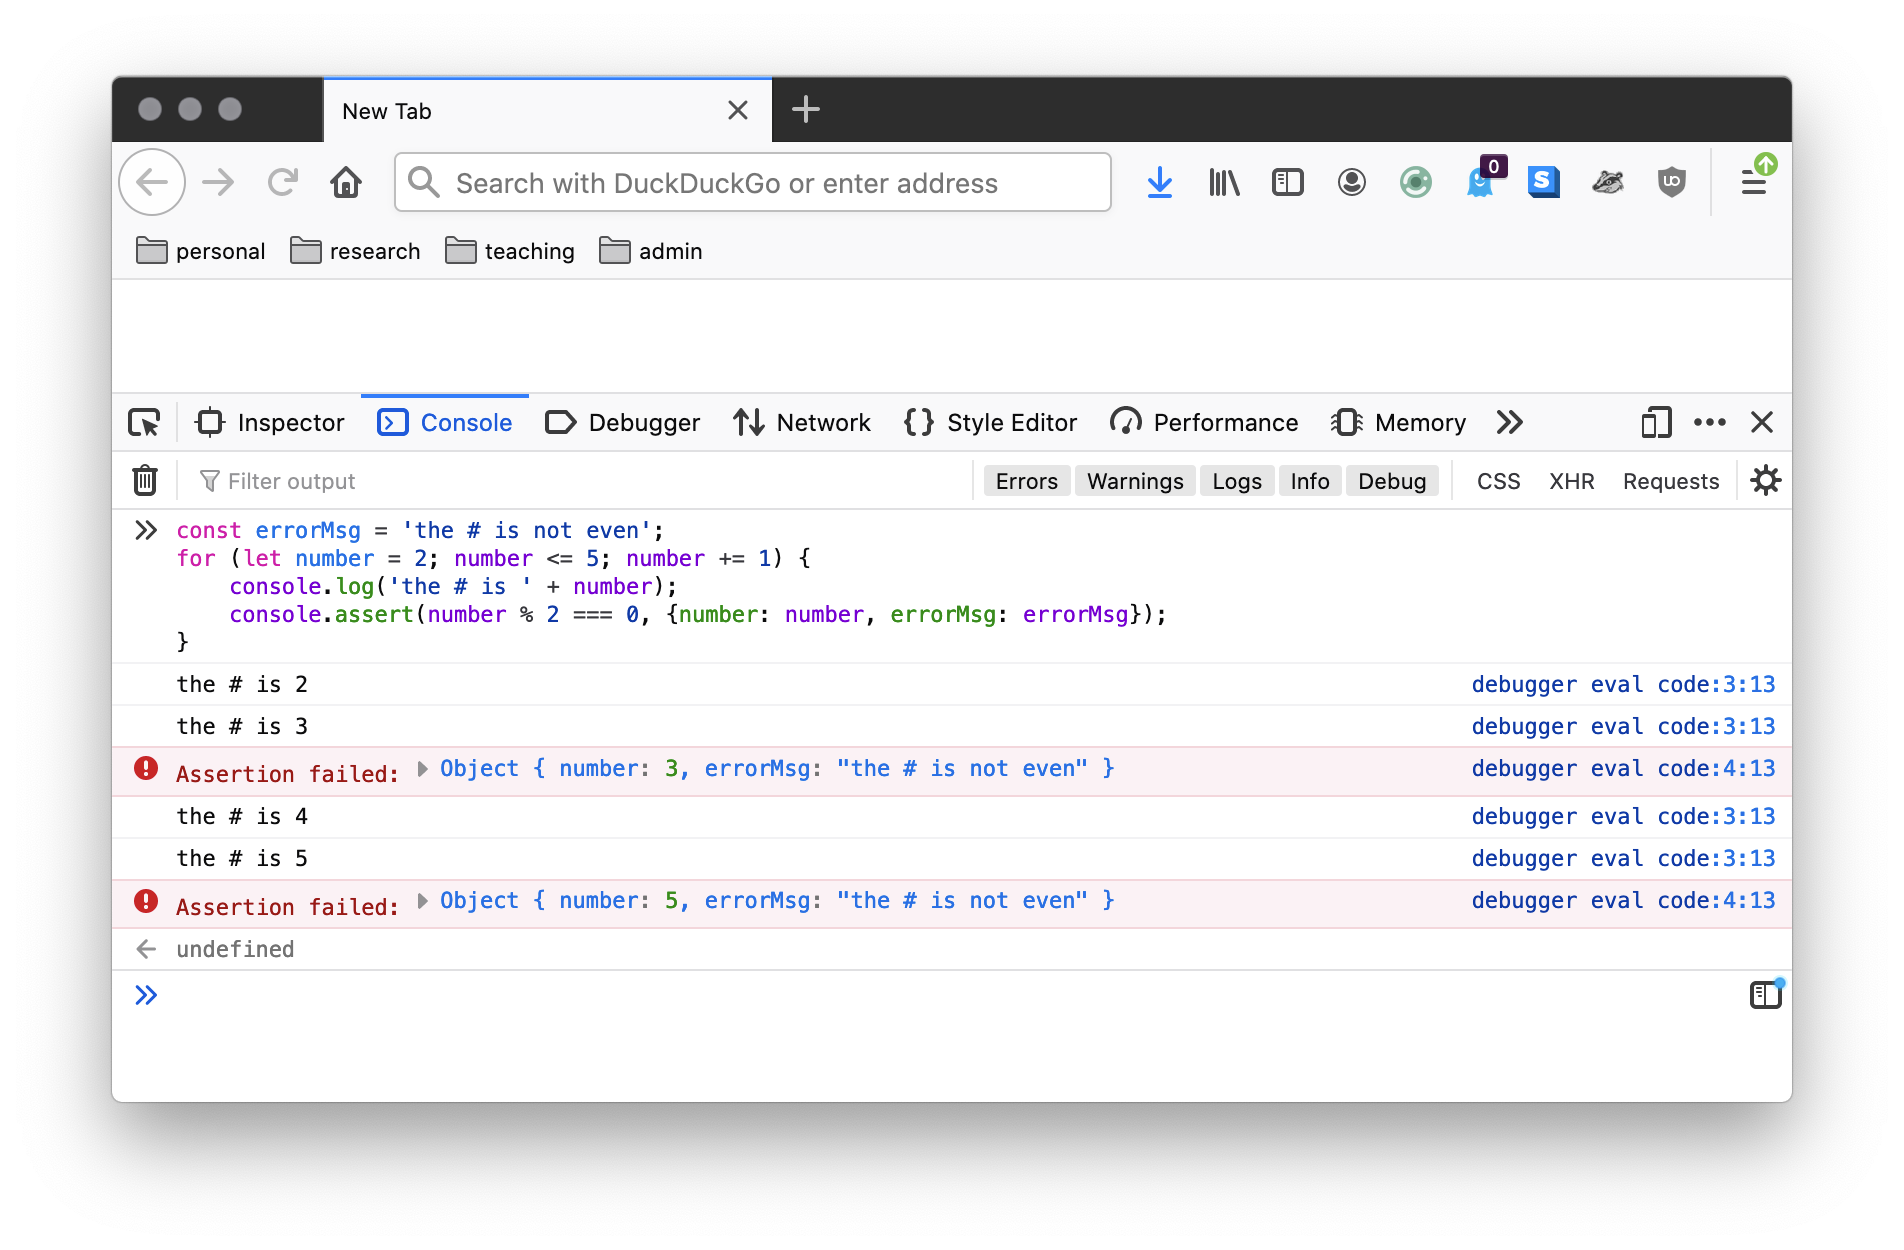
\includegraphics[width=0.8\textwidth]{figures/console-assert}
\label{fig:console-assert}
\caption{}
\end{figure}


\subsection{Console Trace Example}
\paragraph{} Sometimes we want to trace the stack of function calls that have led to the current situation in our running JS code. The console.trace function lets us do this.

\begin{lstlisting}
function foo() {
  function bar() {
    console.trace();
  }
  bar();
}

foo();
\end{lstlisting}

\paragraph{} Running this code in the browser console will give output similar to this:

\begin{figure}[H]
\centering
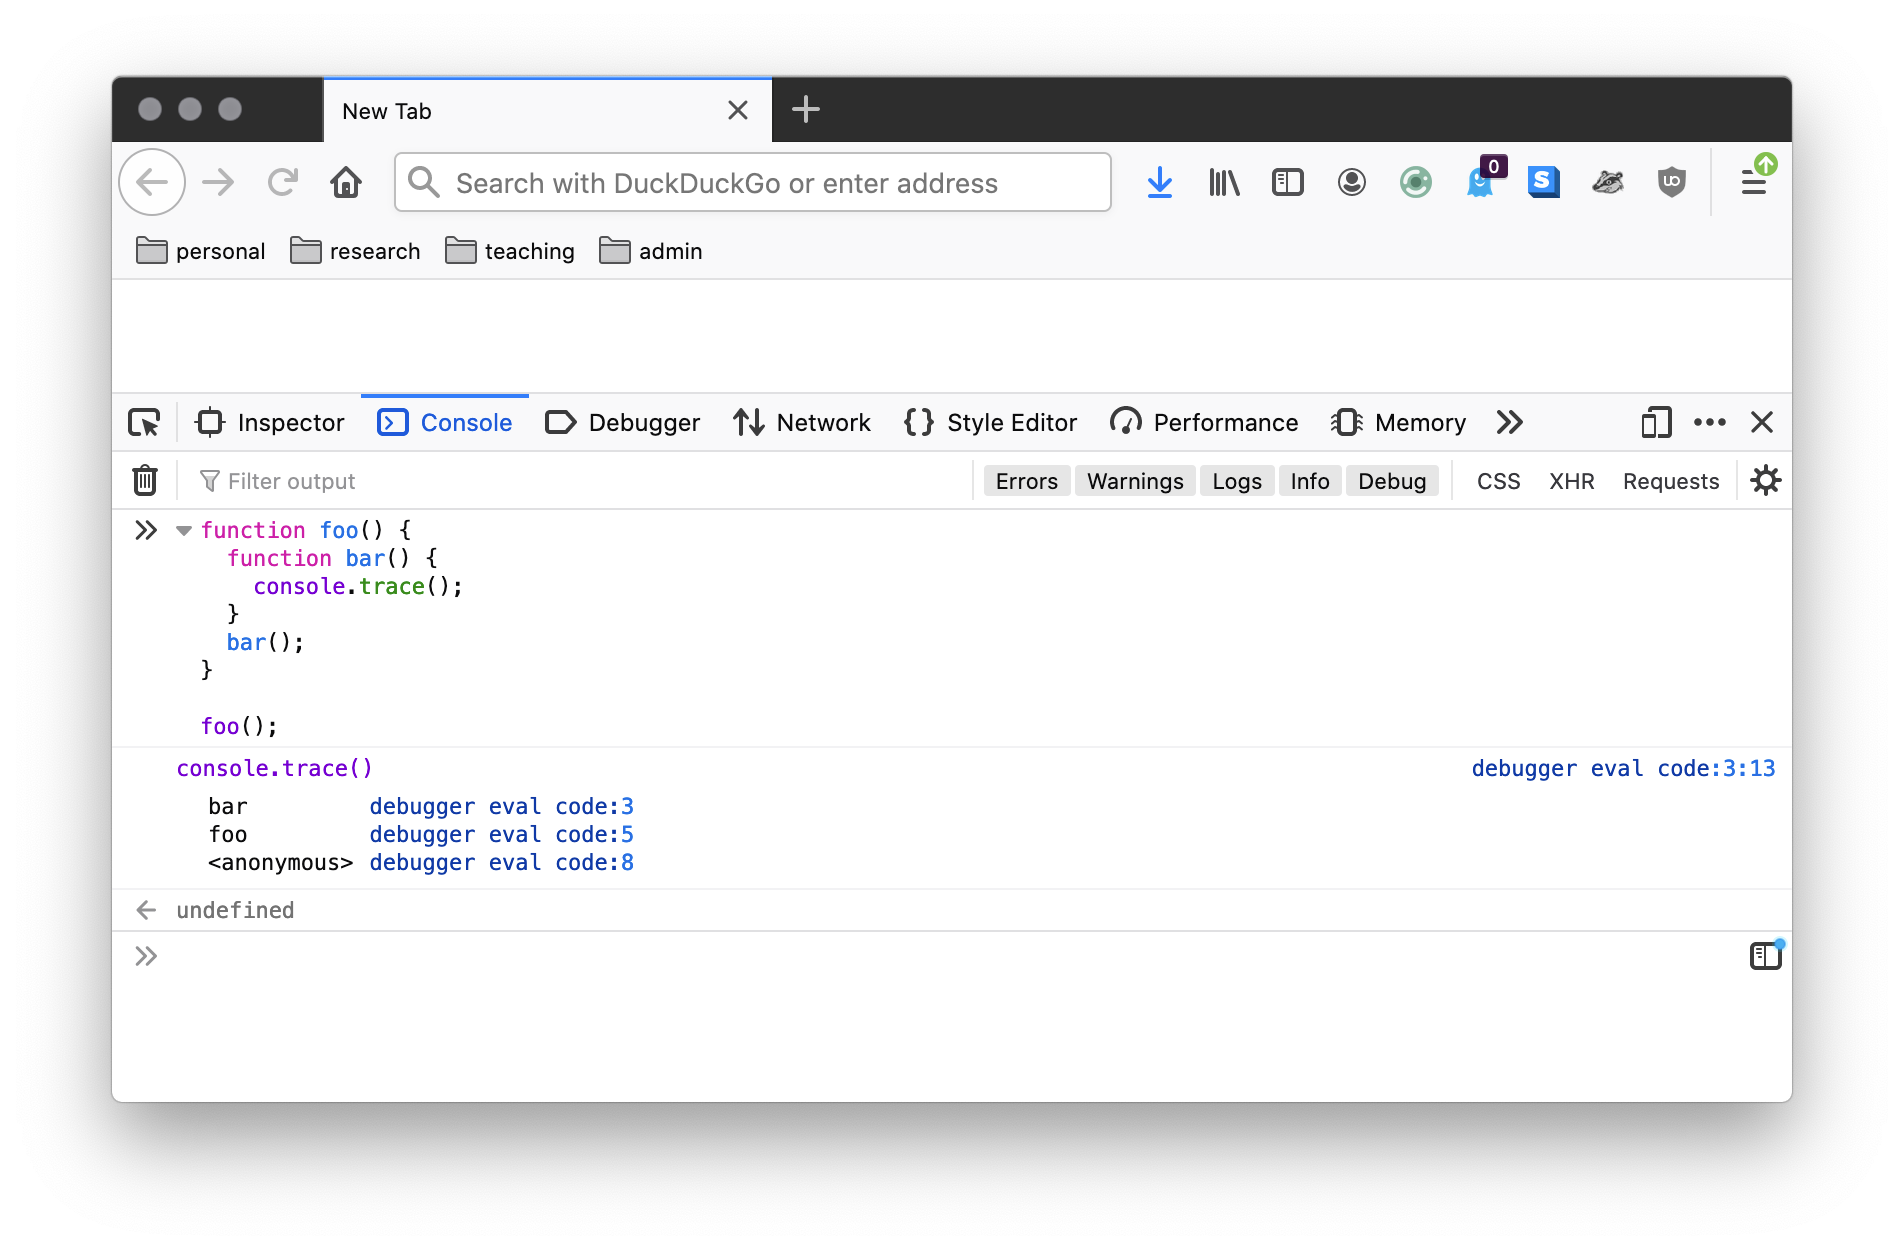
\includegraphics[width=0.8\textwidth]{figures/console-trace}
\label{fig:console-trace}
\caption{}
\end{figure}


\section{History Object}
\paragraph{} Returning to the Window object again, let's examine the History object. This stores the list of URLs that the user has visited within the current browser window or tab. It doesn't give access to other tabs however, only the current one. Access to specific URLs that might previously have been visited is prohibited, as is access to other windows or tabs that the browser might have opened. This is for both security and privacy reasons and aims to keep individual windows and tabs relatively isolated from each other.

\paragraph{} The History Object has the following properties:

\begin{itemize}
\item length -  the number of URLs in the history list
\end{itemize}

\paragraph{} The following methods are also available for use:

\begin{itemize}
\item back() -  Load the previous URL
\item forward() - Load the next URL
\item go() - Load a specific URL from the list by jumping n places (positive or negative) to move that amount through the history list
\end{itemize}

\paragraph{} Note that the history object is not standardised but is supported in the above format by major browsers, so you might find some more esoteric browsers whose behaviours differ.


\section{Navigator Object}

\paragraph{} The Navigator object stores information about the browser. The properties that are available and which can be retrieved include the following list (which is not exhaustive):

\begin{itemize}
\item appName - Returns the browser name
\item appVersion - Returns the version of the browser
\item cookieEnabled - Are cookies enabled?
\item platform - Which OS is this browser installed on?
\item userAgent - Access the header sent by the browser to the server to self identify
\end{itemize}

\paragraph{} Note that again, the navigator object is not standardised but is supported in the above format by most major browsers.


\section{Screen Object}
\paragraph{} Similar to the Navigator object, the screen object is a source of information about the screen that the user’s browser is displayed on. This can be useful, for example, when using different layouts and trying to decide when to switch from one to another.

\paragraph{} The supported properties include:

\begin{itemize}
\item availHeight - Height of screen minus certain furniture, e.g. windows taskbar
\item availWidth - Width of screen minus certain furniture, e.g. windows taskbar
\item height - Total height of the screen
\item pixelDepth - Colour resolution in bits per pixel
\item width - Total width of the screen
\end{itemize}

\paragraph{} Note that, as for the Navigator and History objects, the Screen object is not standardised but is supported in the above format by major browsers (do you notice a theme developing here\ldots?).


\section{Document Object Model}
\paragraph{} Now, having surveyed all of the other child objects of the Window object, let's turn our attention to the Document object and the Document Object Model (DOM). When an HTML file is retrieved and loaded the HTML tags are parsed into a hierarchical data structure, a tree, that more-or-less matches the structure of our HTML. The key difference is that this data structure, the DOM, is easier to manipulate, i.e. from JS code (or CSS). The browser uses the DOM during the rendering process and is a critical underpinning metaphor or model for the way that most modern browsers operate. Once an HTML file is parsed, the browser ignores it and prefers to use only its internal DOM representation of the page. Here is a basic illustration of a simple HTML document parsed into a DOM representation. Obviously things can become much more complex than this.


\begin{figure}[H]
\centering
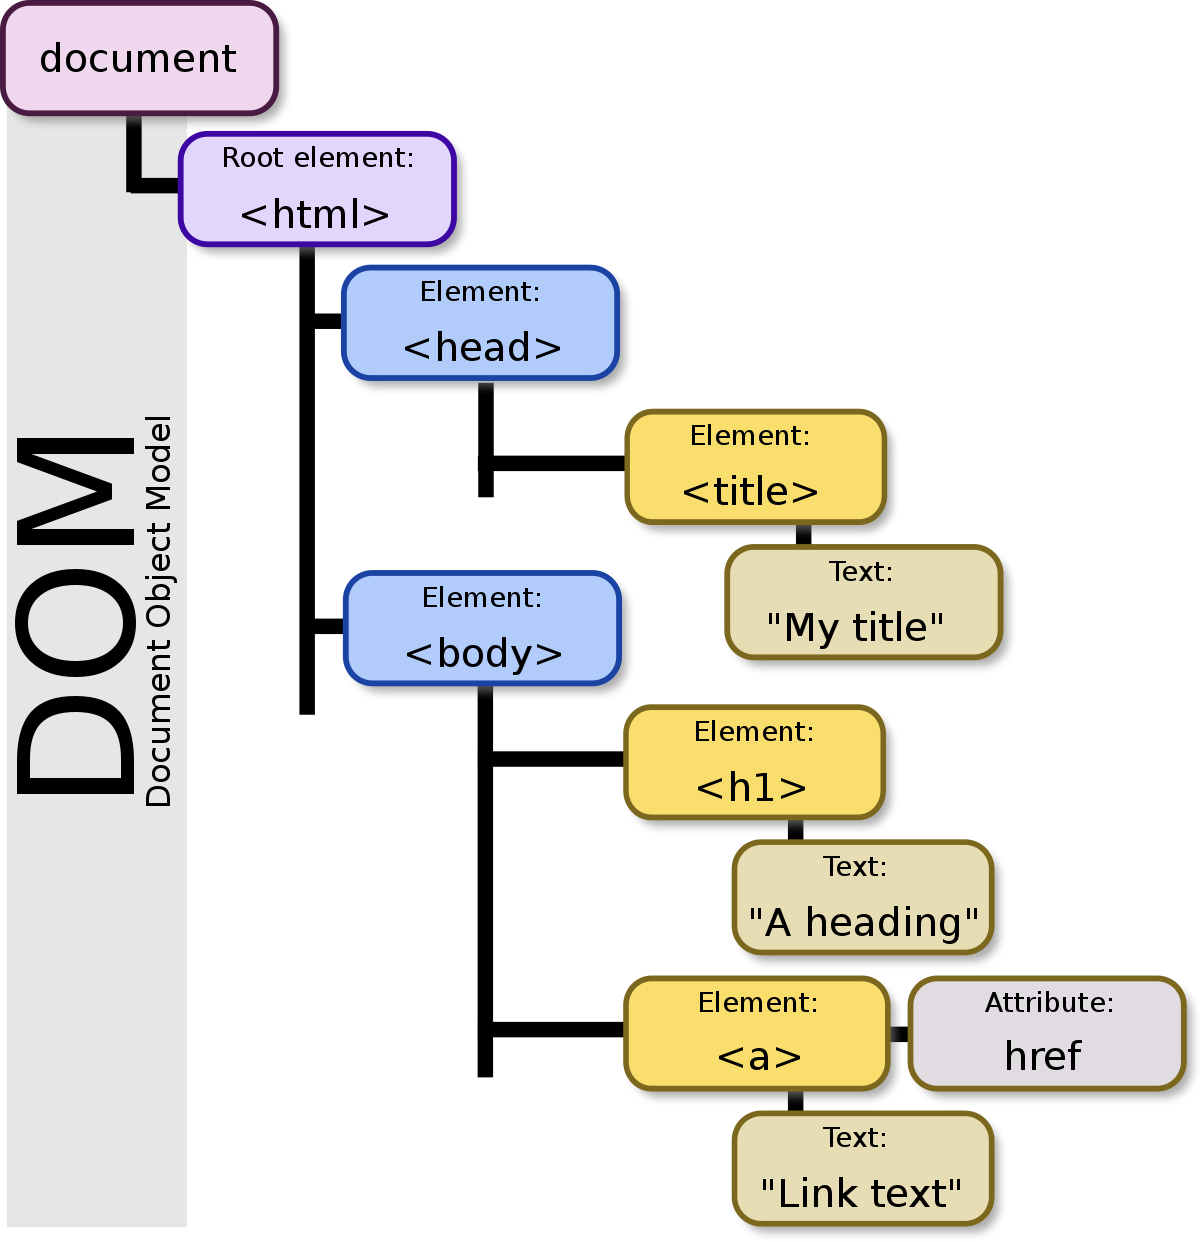
\includegraphics[width=0.8\textwidth]{figures/dom}
\label{fig:dom}
\caption{}
\end{figure}

\section{DOM as API}
\paragraph{} The DOM is a programming interface (API) for HTML. The DOM represents the page so that their structure, style, and content can be changed without needing to change or manipulate the source file(s) that define the page. This means that if we refresh a page, the result is a new instance of the page parsed into a new DOM, regardless of any changes that we'd made before the refresh. Note that this only holds if extra measures haven't been taken to persist any changes, for example, by using a cookie or browser local storage.
\paragraph{} The DOM operates in an Object-oriented way. Logical elements of the page are exposed to the user, who in this case is the programmer, as a containment hierarchy of objects which can, in turn, be modified.
\paragraph{} Be aware that many browsers extend the basic DOM to provide browser specific features but there is a common core that is shared across most modern browsers based upon the standards defined by the W3C and WHATWG.


\section{Accessing the DOM}
\paragraph{} Our browser’s JS environment gives us access to a global document object which we can access through the document object or else via the Window object, e.g. 

\begin{lstlisting}
	window.document
\end{lstlisting}

\paragraph{} Strictly we should access the document object and its contents as follows:

\begin{lstlisting}
	window.document. ...
\end{lstlisting}

\paragraph{} but both the window and document are exposed to JS as global objects so you might either approach both in real world code. As with most things, choose a style and be consistent in your own code, at least within any given project.
\paragraph{} It is a useful exercise to explore the document object in the browser console using the autocomplete function. Type in document and your browser should display a popup list of available attributes and functions that you can explore. This is a useful way to find out what is available on any given page.
\paragraph{} Once you access the DOM via the document object you can subsequently access, and explore, the document’s objects using the dot (“.”) operator.
\paragraph{} Try this out with some of your existing pages that you created earlier. Load one into a tab then open the browser console and explore which elements of your pages are exposed and available for manipulation. You should notice that, for example, the head and the body and the elements that they contain, and so on, are all accessible from JS. It is also worth noticing that what the DOM makes available to you is heavily dependent upon the contents of the specific page that you are on. A different page will likely have a very different DOM representation in terms of the detailed contents of the page, even if the broad structure, head and body, are the same. 
\paragraph{} Using the DOM, we can not only access but also modify, add, or remove elements so that we can change the contents of the current page, or even completely replace all of the HTML content with new content from code.



\section{Accessing Elements}
\paragraph{} One we have access to the DOM via the document or window.document objects we can access the elements within the page using the getElementById function, as we saw in previous examples:

\begin{lstlisting}
<!DOCTYPE html>
	<html> 
		<head>
			<title>SET08101 - Interacting with the DOM</title> 
		</head> 
	<body > 
		<p>
			<a href="#" onClick="addMessage();">Click Me</a>
		</p>
		<h1>OUTPUT:</h1>
		<p id="outputDemo"></p> 
		<script>
		function addMessage() { 
			document.getElementById("outputDemo").innerHTML = "HELLO NAPIER”
			}
		</script> 
	</body> 
</html> 
\end{lstlisting}

\paragraph{} In addition we can use other methods to retrieve elements of the DOM, especially if there isn't a specific ID to use. For example we have:

\begin{itemize}
\item getElementsByClassName()
\item getElementsByName()
\item getElementsByTagName()
\end{itemize}

\paragraph{} Which enable us to retrieve collections of elements that match either the specific class name attribute, name attribute, or tag name. Additionally there are also the querySelector() and querySelectorAll() methods which can be used, respectively, to access either the first element in the DOM that matches a given CSS selector or else all elements that match the supplied CSS selector.


\section{Adding \& Manipulating HTML DOM Elements}
\paragraph{} Just retrieving the contents of the page using the various get methods doesn't really help us much more than we could achieve if we just read the entire web page. So there are also mechanisms to let us manipulate the DOM by adding in new HTML elements, styling them with CSS, or attaching JS code to them. In the following example we create a new $<$h1$>$ element then create some text in a text node. We attach the text node to the $<$h1$>$ element by appending the text  node to it as a new child which causes the child text to effectively be enclosed in the parent $<$h1$>$ tags. The new heading tag and its child text are then appended to the document's body which causes the new heading to be displayed.

\begin{lstlisting}
<html>
  <head>
    <script>
       window.onload = function() {

         const heading = document.createElement("h1");
         const heading_text = document.createTextNode("DAKA DAKA");
         heading.appendChild(heading_text);
         document.body.appendChild(heading);
      }
    </script>
  </head>
  <body>
  </body>
</html>
\end{lstlisting}

\paragraph{} In addition to appending a child, all DOM elements let you manipulate them in a consistent way using the DOM element object API, for example using the various insert methods to place elements specifically in relation to existing elements instead of merely appending them. A summary of available methods for manipulating HTML DOM elements can be found in the W3Schools documentation\footnote{\url{https://www.w3schools.com/jsref/dom_obj_all.asp}}.

	

\section{Resources}
\paragraph{} There are many source of information about the Browser-based JS APIs: 
\begin{itemize}
\item The MDN JS Reference\footnote{\url{https://developer.mozilla.org/bm/docs/Web/JavaScript
}} not only includes reference information but also a set of tutorials for exploring JS
\item W3Schools JS and HTML DOM reference\footnote{\url{https://www.w3schools.com/jsref/}}
\item W3schools JS Tutorial\footnote{\url{https://www.w3schools.com/js/DEFAULT.asp}}
\end{itemize}


\section{Summary}
\paragraph{} In this chapter we've examined the JS APIs that most modern browsers support. Briefly we've considered:
\begin{itemize}
\item Looked at the role that JavaScript plays amongst other web technologies
\item Gained an understanding of the core JavaScript syntax
\item Discovered how JavaScript interacts with HTML, CSS, and the Browser
\end{itemize}


\chapter{Client-Side JS: Data Storage APIs}
\label{data-storage}
\paragraph{} The web is for sharing information and sometimes we want to change the information on webpages and have our changes stick around for longer than our browser tabs are open. In this chapter we'll continue to build on the last two topics, but this time focusing upon a specific set of APIs that the browser makes available for storing data. This is what we can use to save data in the browser so that it is still there if we reload a page, very useful if we want to build a web app with persistent functionality or if we want to create a nice user experience. 
\paragraph{} We’ll examine the broad range of options for web-oriented storage on the client (with a little consideration of the server). This involves not only an awareness of specific technologies like the APIs for cookies or web storage in the browser, but also how client-side JS can make use of databases to persist information and the limitations that working on the client side impose.
\paragraph{} We'll also take a look at the JSON language as the default JS way to describe and structure our data for serialisation.
\paragraph{} Briefly, we'll cover the following major client-side data-storage and data-representation related topics:

\begin{itemize}
\item HTTP Cookies
\item DOM Storage
\item Indexed DB
\item JSON
\end{itemize} 


\section{Client Side Storage \& Data Persistence}
\paragraph{} Data on the web can be ephemeral. We will often visit pages, interact with the contents of the page, and leave without caring that our data is lost. However occasionally we will want to persist our data. This is increasingly true when we consider the move towards web-based applications, as opposed merely to web-sites. Similarly, whenever we offer our user options to personalise their experience, it makes sense to save those options somehow so that when they return, things are still saved the way they left them. Even if they closed all their tabs and restarted their browser in-between, once they revisit our site, their data is as they left it.
\paragraph{} Note however that client-side storage has one major drawback, if a user clears their browser’s cache, or other data storage associated with their browser, then all of the information that we are considering storing on the client side will be lost. This is the main downside to client side storage, but, to be honest, it is a downside that is surrounded by other advantages.
\paragraph{} Generally client side data is already on the client so it makes sense to persist it on the client if only the client needs to reuse that data. This is good enough for many circumstances. However, a more robust solution that allows the user to move between browsers or machines will require data to be stored on a server. Similarly, if you have any functionality that involves aggregating data, such as social media style functionality, then this usually also requires data to be stored on a server. Similarly, moving data to and from the server involves additional steps which can introduce opportunities for your system to either fail, or run in a less than optimal way. However, storing data on a server is outside the remit of this module, and also raises additional considerations related to security and privacy of user's stored data.
\paragraph{} If we architect our sites well then our user's data might never have to leave the client and for many sites, this is perfectly fine.


\section{Client Only Data}
\paragraph{} If the server never sees any data, if it only provides the interface and web-app or site for working with the data entirely on the client side then this simplifies a whole series of issues:

\begin{enumerate}
\item Client side data has good privacy preservation. If a user's data never leaves their browser then it is hard for it to be misused, abused, or lost. This greatly simplifies the legal position for web developers.
\item There is a different security model between client-side only data and data that moves from client to server. In the former, an attacker must target individual clients to access data. In the latter there are more points to target, not only individual clients, but also the server and also the data in transit between client and server.
\item There is no need for potentially expensive data storage or management facilities and no need to determine when to keep data and when to discard it.
\item If data isn't moved to the server then there is no need for user management facilities to support separating data and making it only accessible to the right users.
\end{enumerate}

\paragraph{} However, there are limitations to what you can do if your user's data is only on the client:

\begin{enumerate}
\item There is no way to easily aggregate data and provide facilities based upon that aggregation. This means that crowd based data analysis or features based upon multiple users interacting aren't possible.
\item It's not easy to facilitate user-to-user communication unless mediated by your server, in which case data passes through you possession. This means that putting different users in touch with each other is currently difficult to do. Note that the WebRTC protocol and API have been moving rapidly towards direct browser-to-browser communication but we are not there yet. Expect to see this in the short to medium term and take note that it will have an impact on the design and implementation of web sites.
\end{enumerate}


\section{Ephemeral Client Data}

\paragraph{} There are multiple ways to store data on the client side, that is, within our user's browser. This is regardless of whether any of that data has previously been on a server or whether it has been entirely captured or generated on the client. Our user’s data never has to leave their browser unless there is a good reason for that to happen. One reason is that data in the client can be considered to be ephemeral, lasting perhaps for only a short time, despite the opportunities that developers have to persist data.
\paragraph{}
The shortest that client side data can last is as long as the browser tab is open. Once the tab, or window, is closed any data within it will be lost. Note that some of the data might persist automatically within the browser's cache, but if the page is reopened, even using cached information, a fresh DOM will be created and anything, like user input, from the previous tab, will be lost. Our use of tools like cookies, DOM storage, and IndexedDB are merely means to extend how long this data can last, firstly beyond closing and reopening a tab or refreshing the page, but conceivably much longer.
\paragraph{} Ultimately though, client side data must always be considered, ultimately, as ephemeral. A user might delete their local data, wipe cookies, clear caches, re-install their operating system, or use a site from a different machine. All of these can affect the availability or otherwise of any data that the user has previously created or generated.
\paragraph{} So client side storage should be treated differently to server side storage. To some degree it is permanent storage and will live for as long as needed but there is no guarantee. If we need to persist data beyond the examples listed above then we need to consider saving data outside the browser, to the user’s local file system, or else storing the data on a remote server. Either solution brings its own additional challenges. Note though that it is seldom all or nothing, client side persistence of information can enable a site to continue working even though there is no network connection, so having a default design approach of "offline first" is not a bad idea. This way client side data can be treated as ephemeral, with the expectation that it will be downloaded from or synchronised with a server again if necessary at some point in the future. As a result we should consider this, when appropriate, in our designs of the client side architecture of our sites.


\section{Client Side Options}
\paragraph{} On the client we have three basic options for data storage and persistence. These are, in order of increasing complexity, power, and storage size:

\begin{enumerate}
\item Cookies
\item DOM Storage (also known as local storage or web storage)
\item IndexedDB
\end{enumerate}

\paragraph{} All three are provided by Browser based APIs which are accessible through JS. This means that you can usually investigate, explore and exploit them direct from the browser console, but usually we would do so from JS within a site that we’ve navigated to.

\paragraph{} Cookies are the simplest, a single named string, associated with a given web address that contains  data about the current page. This can be useful for very simple information, such as security tokens, usernames, or small amounts of data like user settings that you want to persist if the page is reloaded. DOM storage is designed to overcome some of the issues with cookies, but at the risk of being slightly more complicated to implement and manage. Whilst cookies are designed primarily for communicating data between client and server (hence the security token suggestion above), DOM storage is designed for client side scripting and data persistence for web apps and isn't communicated to any associated server in the same way that cookie strings are. IndexedDB is the most complex client side data storage mechanism available to us and is an API for managing a NoSQL style database of JSON objects. The amount of data that each can store increased, with cookies supporting the least, and IndexedDB, the most. As the amount of data storage has increased so too has the complexity of each solution, as well as the amount of code needed to effectively manage each approach.

\paragraph{} Let's now look at each in turn, starting with cookies.


\section{Cookies}
\paragraph{} A cookie is a small piece of data that is usually sent from a website server to the client machine/browser where it is then stored. Cookies can also be created, on the client, through JS so can be misused for data persistence solely on the client.
\paragraph{} A cookie is actually a single string and is transmitted in the HTTP headers during client-server communication, for example, as part of the process of retrieving a web page during an HTTP GET transaction.
\paragraph{} Cookies are designed to be a reliable mechanism for maintaining information about state, i.e. keeping track of things across pages during navigation. This enables the stateless nature of the underlying HTTP protocol to be avoided and is a useful and important technique in those circumstances. Cookies can also be used to record activity, such as where you click, your user credentials, your log-in status, your history of interaction on a site, as well as arbitrary information that your pages might need to use, such as names, addresses, etc.
\paragraph{} Cookies have a poor reputation, mainly because they have been greatly misused over the years in privacy and security impacting ways. This has led to laws restricting their use in tracking people and requiring prior notification of their use, through effective informed consent, before non-essential cookies can be used. Note the important point about "non-essential" use however, cookies are perfectly fine to use if they are essential to the functionality of your site and don't track users or otherwise invade their privacy, i.e. you cannot just deem everything to be essential and then not inform your users of their use. The non-essential clause is not a "get out" for ignoring the user notification laws but is a recognition that there are important and valid uses for cookies and that under some circumstances they can and should be used to provide essential functionality.



\section{Creating, Reading, Updating, \& Deleting Cookies}
\paragraph{} Cookies can be created and manipulated in many ways. They are often created on a Web server and then transmitted through the HTTP headers to the client during an HTTP request-response cycle.
\paragraph{} They can also be created through JavaScript using the document.cookie property of the browser API and are thus a useful way to store small volumes of data. Data in a cookie is a name-value pair, e.g.

\begin{lstlisting}
	name = Carol Danvers
\end{lstlisting}

\paragraph{} In JS a cookie can be created very easily using something like this:

\begin{lstlisting}
	document.cookie = "username=Carol Danvers";
\end{lstlisting}

\paragraph{} Cookies can easily be retrieved into a JS variable for the current page, e.g.

\begin{lstlisting}
	var new_cookie = document.cookie;
\end{lstlisting}

\paragraph{} We can also update an existing cookie the same way it is created (causing existing cookie to be overwritten):

\begin{lstlisting}
	document.cookie = “username=Captain Marvel”;
\end{lstlisting}

\paragraph{} Note that we don’t explicitly need to delete cookies, instead we can just set an expiry parameter like so:

\begin{lstlisting}
	document.cookie = “username=; expires=Thu, 01 Jan 1970 00:00:00 UTC; path=/;”;
\end{lstlisting}


\section{DOM/Local/Web Storage}
\paragraph{} DOM storage (also known as local storage or web storage) is a set of APIs to provide persistent storage for use in web apps. Despite the different names, they refer to the same set of APIs and are dependent upon browser support in your user’s client software. We'll refer henceforth to DOM storage for simplicity. Whereas cookies were designed for moving ephemeral user specific data between server and client and vice versa their use for data storage is really a misuse. Dom Storage is designed to support the needs for most client side web apps which need to store data locally.
\paragraph{} DOM storage is similar to cookies but with greater capacity, a cookie is limited to 4KB whereas DomStorage can store  5, 10, or 25MB of data, depending upon platform and browser. DOM storage uses two global JS objects, sessionStorage and localStorage, which provide two related but different levels of data storage functionality.
\paragraph{} The sessionStorage object is for data that is limited to the lifetime of the window and is on a per origin, window, or tab basis. It enables separate instances of the same web application to run in different windows without interfering with each other.
\paragraph{} The localStorage object is persistent after the browser closes and is per origin where origin is a combination of protocol, hostname, and port number. A localstorage object instance is available to all scripts loaded from pages with the same origin and therefore is useful if you need multiple pages, for example, multiple instances of the same web-app in different tabs, to share data amongst themselves.

\paragraph{} We can store a value for the rest of a session very simply:

\begin{lstlisting}
	sessionStorage.setItem(‘key’, ‘value’);
\end{lstlisting}

\paragraph{} Then we can retrieve a value later by supplying the key (so we need to keep track of keys or have a way to supply them within our web-apps):

\begin{lstlisting}
	alert(sessionStorage.getItem(‘key’));
\end{lstlisting}

\paragraph{} Note that localstorage works in an almost identical fashion, just with different object names to differentiate local from session.
\paragraph{} Store a value beyond current session:

\begin{lstlisting}
	localStorage.setItem(‘key’, ‘value’);
\end{lstlisting}

\paragraph{} Retrieve value:

\begin{lstlisting}
	alert(localStorage.getItem(‘key’));
\end{lstlisting}



\section{Indexed DB}
\paragraph{} Indexed DB is a W3C recommended standard for a low-level browser API for client-side storage of a local, transactional database. This is essentially a full-blown database hosted in our browser rather than merely a key-value datastore. This enables sites to “permanently” collect and save large amounts of structured data. Note that our notion of permanence here is still subject to the discussion of ephemeral data from earlier.
\paragraph{} Indexed DB is a form of NoSQL storage and basically creates collections of indexed  JSON objects. There is preliminary support in many browsers, including, Firefox, Chrome, Safari but it is worth allowing the technology to mature somewhat before you rely upon it. As a result it is included here for reference and completion, and to prepare you for the future.
\paragraph{} Indexed DB promises a lot of power for data storage and manipulation in our web apps. It is aimed at browser implemented functions (such as bookmarks) and web applications (like email clients). For our purposes, and most websites, Indexed DB is overkill where DOM Storage or alternatives that are hosted entirely within JS, like PouchDB, JsStore, \&c., are more appropriate


\section{JavaScript Object Notation (JSON)}
\paragraph{} Now we need to take a slight diversion to fill in a gap in our knowledge. We’ve mentioned JSON very briefly in passing so far, but as we start to build more feature rich sites, we'll have more data to structure, to manipulate, and to store. Our data won't live all of its time within our code or within working memory, so serialisation formats can be useful. "Serialisation" is just a fancy term that is used to describe turning the data used within a program into a form that is better suited for other purposes, like storage, or human inspection, outside of the running program.
\paragraph{} Although it was originally developed for serialising JS Objects, JSON is now a de facto generalised standard for describing data, particularly in the Web, but also, increasingly, within many other computing scenarios, e.g. saving data from a desktop application, transmitting data across a network, or saving data from instruments or sensors.
\paragraph{} Data is often sent to web-apps, and retrieved from web-apps, in JSON format. There are other formats but JSON has become the default, probably due to the close relationship between JSON and JS. Data is often also stored as JSON either in the filesystem or in data-stores. Data is often manipulated within JS as JSON. As a result we should probably take a closer look at it.
\paragraph{} JSON is an acronym for JavaScript Object Notation and it is yet another language, but the last one we'll consider for this module. Really though, it is so closely related to its parent JS that if we have gotten to grips with JS, and specifically with JS objects, arrays, and variables then JSON itself should not present any major surprises. Really, if you already know JS then JSON can be considered as more of a different perspective on some things that you should already know than as a new language. JSON is basically a transliteration from objects within JS into a plain text format that can be saved and reused in other contexts including outside of JS. Note that JSON within JS and JSON outwith JS look almost identical in practice. So if you have become familiar with JS objects then JSON isn’t going to be a huge challenge.
\paragraph{} It's worth also relating JSON to HTML. Neither is a general purpose programming language, they both lack features necessary to be programming languages, but they are both used for specific tasks related to describing data. In the case of HTML, for describing the structure of human knowledge in the form of hierarchically organised text documents, and in the case of JSON, for describing hierarchically organised collections and structure of knowledge.



\section{JSON Examples}
\paragraph{} Before looking in more detail at JSON as a language, it is worth seeing an example of some actual JSON first and comparing it to the equivalent JS object. The following should look reasonably familiar from our previous discussion of JS objects:

\begin{lstlisting}
var cow = {
	name: “daisy",
	likes: “clover”, 
	moo:function() {
		console.log(‘moo’);
	}
};
\end{lstlisting}

\paragraph{} This is our construction of a JS object to represent our cow "Daisy". Daisy has a name attribute and an attribute that describes something she likes. Daisy also has a function, moo, because all cows moo.
\paragraph{} In the following example we see the JSON serialisation of the Daisy cow object:

\begin{lstlisting}
{
	“name”:”daisy",
	“likes”:”clover”
}
\end{lstlisting}

\paragraph{} That's it. That's our Daisy object described in JSON. Notice that only Daisy's attributes are recorded in our JSON document. The function has been discarded. Only data, or attributes are stored in JSON files so we might have to account for this in our programming. This is a pretty-printed example of JSON which uses whitespace and indentation to show the structure of the data for human readers. Frequently though, you might see JSON represented like this:

\begin{lstlisting}
{ “name”:”daisy", “likes”:”clover” }
\end{lstlisting}

\paragraph{} Everything is presented inline and without additional formatting to make it easier to read. Sometimes you might need to copy such examples into a tool like JSONLint (which we'll see later) to get the JSON to be automatically checked and structured for better human readability.



\section{JS $\longleftrightarrow$ JSON}
\paragraph{} We can move backwards and forward between JS objects and JSON using some standard JS functions. We can use JSON.stringify to turn a JS object into a JSON string:

\begin{lstlisting}
	JSON.stringify(js_object);
\end{lstlisting}

\paragraph{} More formally, this will serialise the JS object ``js\_object'' into a string. For the moment let's just consider a string to be a linear sequence of characters that are enclosed within double quotes but soon we'll see more formally, in a railroad diagram, the full extent of the range of characters that can be used to build a valid JSON string.

\paragraph{} We can also take an arbitrary, but correctly formed JSON string and parse that into a JS object hierarchy using the JSON.parse function:

\begin{lstlisting}
	JSON.parse(json_string);
\end{lstlisting}

\paragraph{} This will parse, or ``read and interpret'', the string identified by ``json\_string'' and construct a JS object hierarchy for use in our program.

\paragraph{} For our purposes, if we want to manipulate data (JSON) in code then our data needs to be parsed from its string representation and turned into an object within our program. Conversely, if we want to store data from our program or send it elsewhere, such as to an API that consumes JSON data, then we need to stringify our JS objects into a JSON document.

\paragraph{} Note that in practice it's not always quite that simple, but it is sufficient for our purposes on this module and for most client side web development.



\section{JSON as a JS-independent Language}
\paragraph{} Rather than being an ad-hoc serialisation of JS Objects, JSON has also been formalised and standardised in its own right. JSON can be used standalone to describe the structure of data and, as a result, is now used in many non-Web and non-JS contexts as a general purpose data description language. So a comparison to other such languages and formats, like XML, YAML, and RDF, to name just three, is appropriate.
\paragraph{} It is fairly straightforward to describe the main points of JSON:

\begin{itemize}
\item JSON is a plain text format. You can create and edit JSON using just your text editor. This is easier once you are used to what the language allows. In the meantime, using a tool like JSONLint.com (which we'll see soon) can be useful in helping you to get it right. That said JSON is not a general purpose programming language, it doesn't let you do iteration or selection or evaluation of data, it just enables you to describe it. If you already know JS and are familiar with JS objects and variables then JSON should make plenty of sense.
\item A JSON document is iteratively constructed. You start with either an object {} or an array [] and then add values to them (including possibly other sub-objects or sub-arrays) ad infinitum until you have described everything you need to describe.
\item A JSON array can store a comma separated list of values.
\item A JSON Object can store a comma separated list of key:value pairs.
\item JSON Values are objects, arrays, strings, numbers, booleans, or null
\end{itemize}

\paragraph{} Even if you build a JSON document independently from your JS, you can still read that into your JS programs and instantiate a collection of data or objects for use within your program.
\paragraph{} An easier way to see how all of this fits together is to visualise the language using railroad diagrams which is what we'll see next.



\section{JSON RailRoad Diagrams}
\paragraph{} Railroad diagrams are a useful way to understand formal programming languages. Just like a train on rail tracks, which has no choice but to follow the tracks, these diagrams are designed to be read by following the line omissions from one side (in this case starting on the left) to the other. The tracks branch and rejoin in ways that allow only certain words or constructs from the language to be included at any given time, and support sequence, repetition, and omission of words in line with those allowed by the language.
\paragraph{} A Valid JSON document contains either an object or an array, construction of which is shown in the following two diagrams. The first diagram shows us how to build an object, and the second, how to build an array. An array is a comma separated list of zero or more values, all enclosed in a set of square brackets. Meanwhile an object is a comma separated list of zero or more string:value pairs, this time enclosed in curly braces.


\begin{figure}[H]
\centering
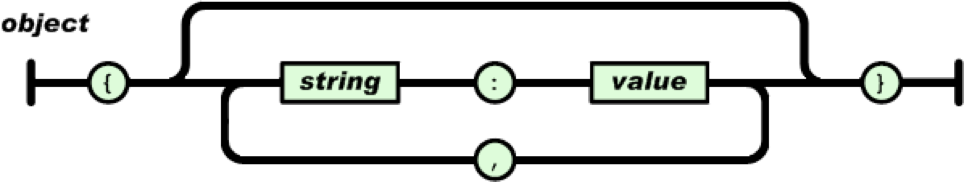
\includegraphics[width=0.8\textwidth]{figures/json-object}
\label{fig:json-object}
\caption{}
\end{figure}

\begin{figure}[H]
\centering
\includegraphics[width=0.8\textwidth]{figures/json-array}
\label{fig:json-array}
\caption{}
\end{figure}

\paragraph{} The values supported by JSON, together with the railroad mechanisms for constructing strings and numbers are given in the following diagrams.


\begin{figure}[H]
\centering
\includegraphics[width=0.8\textwidth]{figures/json-value}
\label{fig:json-value}
\caption{}
\end{figure}

\begin{figure}[H]
\centering
\includegraphics[width=0.8\textwidth]{figures/json-string}
\label{fig:json-string}
\caption{}
\end{figure}

\begin{figure}[H]
\centering
\includegraphics[width=0.8\textwidth]{figures/json-number}
\label{fig:json-number}
\caption{}
\end{figure}



\section{JSONLint}
\paragraph{} Linters are useful tools that are available for most programming languages. They are usually fairly simple programs that you can use to flag up programming errors. The kinds of errors that a Linter might bring to your attention can include syntax errors, certain kinds of bugs, stylistic issues, and various kinds of "code smell". Note that Linters can't (yet) check for more complicated or subtle bugs, for example, those arising from logical errors of reasoning that stem from the programmer, or from errors that arise because the problem and solution are underspecified, or because the programmer isn't sure what their goal is. Whenever you learn a new programming language it is worth looking for a linter tool to support you in using the language correctly and picking up on simple issues. Note that there is some overlap between a linter and the kinds of checks that some compilers and interpreters do but rather than going through the entire build process, which can be time consuming, a linter can process your source code and more rapidly give useful immediate feedback about certain categories of problems.
\paragraph{} JSONLint\footnote{\url{https://jsonlint.com/}} is a very useful online tool for quickly editing ad validating JSON files. You can find it here:	
\paragraph{} It's really simple to use, edit some JSON either in your own files then copy/pasting or directly into JSONLint's interface then press the "Validate JSON" button. The JSON is either valid or else you will be shown where the error lies. Once everything is fixed then you can copy and paste the nicely formatted JSON data back to your own text file and save for usage elsewhere.

\begin{figure}[H]
\centering
\includegraphics[width=0.8\textwidth]{figures/jsonlint}
\label{fig:jsonlint}
\caption{}
\end{figure}

\paragraph{} Note that JSONLint is also great for when you receive JSON from elsewhere, perhaps as the result of an API call. JSONLint will format the JSON and enable you to more easily see the structure of the data within the JSON document.


\section{Why is JSON important?}
\paragraph{} If you are going to build APIs, or really exploit JavaScript, or share data with other APIs (or retrieve data from them) then you will need to use JSON. Really, you can't effectively use JavaScript objects without getting a crash-course in JSON anyway, but JSON also has a role beyond being the text based serialisation format of JSON objects.
\paragraph{} There are many other data transport and representation languages, e.g. XML, YAML, RDF, but JSON occupies a sweet spot that:

\begin{itemize}
\item is not too complex — so you can get up and running swiftly and can quickly prototype ideas.
\item tooling is lightweight — you don't need any specialist tools, you can just write JSON into a regular text file (although as we saw earlier a Linter tool can be useful to help avoid simple mistakes).
\item is human readable — you should be able to read through a JSON document and interpret the structure of the data that it describes. If a JSON file isn't easily readable then that is usually either a failure of the developer of the file to ensure that it correctly communicates the data or else means that there is some specialist knowledge required to interpret the actual data itself, unrelated to the JSON representation.
\end{itemize}

\paragraph{} Yes, there are drawbacks to JSON (stackoverflow is a great place to find discussions between professional developers on the merits, or otherwise, of JSON), but the positives make it an easy tool to choose and use. This is probably why JSON is frequently a go to choice for data description and representation even amongst developers who are not doing web development or using JavaScript.

\section{Resources}
\paragraph{} As usual, due to the rapid pace of change in web technologies, the best place to get up to date information about the current status of browser related data storage APIs is from the Mozilla and Google documentation.

\begin{itemize}
\item MDN Cookie API\footnote{\url{https://developer.mozilla.org/en-US/docs/Web/API/Document/cookie}}
\item MDN Web Storage API\footnote{\url{https://developer.mozilla.org/en-US/docs/Web/API/Web_Storage_API}}
\item MDN Indexed DB API Documentation\footnote{\url{https://developer.mozilla.org/en-US/docs/Web/API/IndexedDB_API}}
\item Google Developers Documentation (Indexed DB)\footnote{\url{https://developers.google.com/web/ilt/pwa/working-with-indexeddb}}
\end{itemize}

\section{Summary}
\paragraph{} In this chapter we’ve looked at the following broad topics:
\begin{itemize}
\item Identified the current main approaches to data storage for the web
\item Distinguished between server-side and client-side data storage
\item Made appropriate choices about which technology to select for a given problem
\end{itemize}


\chapter{Client-Side JS: Sound \& Vision APIs}
\label{sound-and-vision}
\paragraph{} 


\chapter{Deployment}
\label{deployment}
\paragraph{} 


\chapter{Conclusion}
\label{conclusion}
\paragraph{} We've surveyed a whole lot of topics so far which should lead to a number of conclusions. Firstly, we can't learn everything about the Web from one book. Instead, this one book is just a starting place, but the onus is on you to keep up-to-date with new developments in the field. The second take away is that the Web is a fast moving collection of technologies that have changed over time, and will continue to change. Ultimately, the Web is a reflection of humanity's desire to share information, and to find better ways to use technology to do so. Perhaps that story started when we daubed pigments onto cave walls, or scratched images onto rocks, or perhaps it was with the development of writing systems, or event he printing press. Regardless, that story has not finished yet, and perhaps never will.




%%%%%%%%%%%%%%%%%
%%%%%%%%%%%%%%%%%
% APPENDICES 
%%%%%%%%%%%%%%%%%
%%%%%%%%%%%%%%%%%

%\part{Appendices}

%\appendix
%\chapter{Cribsheets}
%\label{cribsheets}
%\paragraph{} These cribsheets are useful for collecting together lots of knew syntax but are no substitute for your own notes (and practise. Stuff you know is much better than stuff you can look up). Either way, as you learn new stuff you should expand these cribsheets with extra commands that you find useful.




\backmatter

\bibliographystyle{plain}

\bibliography{bib/webtech}

\end{document}


